\documentclass[twoside]{book}

% Packages required by doxygen
\usepackage{fixltx2e}
\usepackage{calc}
\usepackage{doxygen}
\usepackage[export]{adjustbox} % also loads graphicx
\usepackage{graphicx}
\usepackage[utf8]{inputenc}
\usepackage{makeidx}
\usepackage{multicol}
\usepackage{multirow}
\PassOptionsToPackage{warn}{textcomp}
\usepackage{textcomp}
\usepackage[nointegrals]{wasysym}
\usepackage[table]{xcolor}

% Font selection
\usepackage[T1]{fontenc}
\usepackage[scaled=.90]{helvet}
\usepackage{courier}
\usepackage{amssymb}
\usepackage{sectsty}
\renewcommand{\familydefault}{\sfdefault}
\allsectionsfont{%
  \fontseries{bc}\selectfont%
  \color{darkgray}%
}
\renewcommand{\DoxyLabelFont}{%
  \fontseries{bc}\selectfont%
  \color{darkgray}%
}
\newcommand{\+}{\discretionary{\mbox{\scriptsize$\hookleftarrow$}}{}{}}

% Page & text layout
\usepackage{geometry}
\geometry{%
  a4paper,%
  top=2.5cm,%
  bottom=2.5cm,%
  left=2.5cm,%
  right=2.5cm%
}
\tolerance=750
\hfuzz=15pt
\hbadness=750
\setlength{\emergencystretch}{15pt}
\setlength{\parindent}{0cm}
\setlength{\parskip}{3ex plus 2ex minus 2ex}
\makeatletter
\renewcommand{\paragraph}{%
  \@startsection{paragraph}{4}{0ex}{-1.0ex}{1.0ex}{%
    \normalfont\normalsize\bfseries\SS@parafont%
  }%
}
\renewcommand{\subparagraph}{%
  \@startsection{subparagraph}{5}{0ex}{-1.0ex}{1.0ex}{%
    \normalfont\normalsize\bfseries\SS@subparafont%
  }%
}
\makeatother

% Headers & footers
\usepackage{fancyhdr}
\pagestyle{fancyplain}
\fancyhead[LE]{\fancyplain{}{\bfseries\thepage}}
\fancyhead[CE]{\fancyplain{}{}}
\fancyhead[RE]{\fancyplain{}{\bfseries\leftmark}}
\fancyhead[LO]{\fancyplain{}{\bfseries\rightmark}}
\fancyhead[CO]{\fancyplain{}{}}
\fancyhead[RO]{\fancyplain{}{\bfseries\thepage}}
\fancyfoot[LE]{\fancyplain{}{}}
\fancyfoot[CE]{\fancyplain{}{}}
\fancyfoot[RE]{\fancyplain{}{\bfseries\scriptsize 構築\+: Doxygen }}
\fancyfoot[LO]{\fancyplain{}{\bfseries\scriptsize 構築\+: Doxygen }}
\fancyfoot[CO]{\fancyplain{}{}}
\fancyfoot[RO]{\fancyplain{}{}}
\renewcommand{\footrulewidth}{0.4pt}
\renewcommand{\chaptermark}[1]{%
  \markboth{#1}{}%
}
\renewcommand{\sectionmark}[1]{%
  \markright{\thesection\ #1}%
}

% Indices & bibliography
\usepackage{natbib}
\usepackage[titles]{tocloft}
\setcounter{tocdepth}{3}
\setcounter{secnumdepth}{5}
\makeindex

% Hyperlinks (required, but should be loaded last)
\usepackage{ifpdf}
\ifpdf
  \usepackage[pdftex,pagebackref=true]{hyperref}
\else
  \usepackage[ps2pdf,pagebackref=true]{hyperref}
\fi
\hypersetup{%
  colorlinks=true,%
  linkcolor=blue,%
  citecolor=blue,%
  unicode%
}

% Custom commands
\newcommand{\clearemptydoublepage}{%
  \newpage{\pagestyle{empty}\cleardoublepage}%
}

\usepackage{caption}
\captionsetup{labelsep=space,justification=centering,font={bf},singlelinecheck=off,skip=4pt,position=top}

%===== C O N T E N T S =====

\begin{document}

% Titlepage & ToC
\hypersetup{pageanchor=false,
             bookmarksnumbered=true,
             pdfencoding=unicode
            }
\pagenumbering{alph}
\begin{titlepage}
\vspace*{7cm}
\begin{center}%
{\Large Fbx\+Converter \\[1ex]\large version 1.\+1 }\\
\vspace*{1cm}
{\large 構築\+: Doxygen 1.8.14}\\
\end{center}
\end{titlepage}
\clearemptydoublepage
\pagenumbering{roman}
\tableofcontents
\clearemptydoublepage
\pagenumbering{arabic}
\hypersetup{pageanchor=true}

%--- Begin generated contents ---
\chapter{トップページ}
\label{index}\hypertarget{index}{}\hypertarget{index_概要}{}\section{概要}\label{index_概要}
F\+B\+Xから\+Direct\+Xと\+Open\+G\+Lそれぞれで使いたいデーターを抽出し、boost\+::serializationでシリアライズ化します。

コンバートした際、そのログデータも出力します。 \hypertarget{index_ライセンス}{}\subsection{ライセンス}\label{index_ライセンス}
Paddington is licensed under the M\+IT license. ~\newline


Copyright \copyright{} 2019 Kai Araki \begin{DoxyAuthor}{著者}
Kai Araki ~\newline

\end{DoxyAuthor}
\begin{DoxyDate}{日付}
2019/01/24 
\end{DoxyDate}

\chapter{クラス索引}
\section{クラス一覧}
クラス・構造体・共用体・インターフェースの一覧です。\begin{DoxyCompactList}
\item\contentsline{section}{\mbox{\hyperlink{class_md_bin_data_1_1_mesh_1_1_bone}{Md\+Bin\+Data\+::\+Mesh\+::\+Bone}} \\*ボーン\+Class }{\pageref{class_md_bin_data_1_1_mesh_1_1_bone}}{}
\item\contentsline{section}{\mbox{\hyperlink{class_md_bin_data_1_1_mesh_1_1_bone_weight}{Md\+Bin\+Data\+::\+Mesh\+::\+Bone\+Weight}} \\*ボーン重み\+Class }{\pageref{class_md_bin_data_1_1_mesh_1_1_bone_weight}}{}
\item\contentsline{section}{\mbox{\hyperlink{class_md_bin_data_1_1_color}{Md\+Bin\+Data\+::\+Color}} \\*色\+Class }{\pageref{class_md_bin_data_1_1_color}}{}
\item\contentsline{section}{\mbox{\hyperlink{class_export_file}{Export\+File}} \\*ファイル出力\+Class }{\pageref{class_export_file}}{}
\item\contentsline{section}{\mbox{\hyperlink{class_fbx_converter}{Fbx\+Converter}} \\*F\+B\+X変換器\+Class }{\pageref{class_fbx_converter}}{}
\item\contentsline{section}{\mbox{\hyperlink{class_md_bin_data_1_1_material}{Md\+Bin\+Data\+::\+Material}} \\*マテリアル\+Class }{\pageref{class_md_bin_data_1_1_material}}{}
\item\contentsline{section}{\mbox{\hyperlink{class_md_bin_data_1_1_matrix}{Md\+Bin\+Data\+::\+Matrix}} \\*行列\+Class }{\pageref{class_md_bin_data_1_1_matrix}}{}
\item\contentsline{section}{\mbox{\hyperlink{class_md_bin_data}{Md\+Bin\+Data}} \\*バイナリーモデルデータ\+Class }{\pageref{class_md_bin_data}}{}
\item\contentsline{section}{\mbox{\hyperlink{class_md_bin_data_1_1_mesh}{Md\+Bin\+Data\+::\+Mesh}} \\*メッシュ\+Class }{\pageref{class_md_bin_data_1_1_mesh}}{}
\item\contentsline{section}{\mbox{\hyperlink{class_md_bin_data_1_1_material_1_1_texture}{Md\+Bin\+Data\+::\+Material\+::\+Texture}} \\*テクスチャ\+Class }{\pageref{class_md_bin_data_1_1_material_1_1_texture}}{}
\item\contentsline{section}{\mbox{\hyperlink{class_md_bin_data_1_1_mesh_1_1_u_v_set}{Md\+Bin\+Data\+::\+Mesh\+::\+U\+V\+Set}} \\*U\+Vセット\+Class }{\pageref{class_md_bin_data_1_1_mesh_1_1_u_v_set}}{}
\item\contentsline{section}{\mbox{\hyperlink{class_md_bin_data_1_1_vector2}{Md\+Bin\+Data\+::\+Vector2}} \\*ベクター2\+Class }{\pageref{class_md_bin_data_1_1_vector2}}{}
\item\contentsline{section}{\mbox{\hyperlink{class_md_bin_data_1_1_vector3}{Md\+Bin\+Data\+::\+Vector3}} \\*ベクター3\+Class }{\pageref{class_md_bin_data_1_1_vector3}}{}
\end{DoxyCompactList}

\chapter{ファイル索引}
\section{ファイル一覧}
ファイル一覧です。\begin{DoxyCompactList}
\item\contentsline{section}{C\+:/\+H\+A\+L/\+P\+G関係/03\+\_\+作成プログラム/03\+\_\+\+H\+A\+L授業/就職作品/\+Fbx\+Converter/source/\mbox{\hyperlink{main_8cpp}{main.\+cpp}} \\*メイン }{\pageref{main_8cpp}}{}
\item\contentsline{section}{C\+:/\+H\+A\+L/\+P\+G関係/03\+\_\+作成プログラム/03\+\_\+\+H\+A\+L授業/就職作品/\+Fbx\+Converter/source/\+Export\+File/\mbox{\hyperlink{_export_file_8cpp}{Export\+File.\+cpp}} \\*ファイル出力\+Class }{\pageref{_export_file_8cpp}}{}
\item\contentsline{section}{C\+:/\+H\+A\+L/\+P\+G関係/03\+\_\+作成プログラム/03\+\_\+\+H\+A\+L授業/就職作品/\+Fbx\+Converter/source/\+Export\+File/\mbox{\hyperlink{_export_file_8h}{Export\+File.\+h}} \\*ファイル出力\+Class }{\pageref{_export_file_8h}}{}
\item\contentsline{section}{C\+:/\+H\+A\+L/\+P\+G関係/03\+\_\+作成プログラム/03\+\_\+\+H\+A\+L授業/就職作品/\+Fbx\+Converter/source/\+Fbx\+Converter/\mbox{\hyperlink{_fbx_converter_8cpp}{Fbx\+Converter.\+cpp}} \\*F\+B\+X変換器\+Class }{\pageref{_fbx_converter_8cpp}}{}
\item\contentsline{section}{C\+:/\+H\+A\+L/\+P\+G関係/03\+\_\+作成プログラム/03\+\_\+\+H\+A\+L授業/就職作品/\+Fbx\+Converter/source/\+Fbx\+Converter/\mbox{\hyperlink{_fbx_converter_8h}{Fbx\+Converter.\+h}} \\*F\+B\+X変換器\+Class }{\pageref{_fbx_converter_8h}}{}
\item\contentsline{section}{C\+:/\+H\+A\+L/\+P\+G関係/03\+\_\+作成プログラム/03\+\_\+\+H\+A\+L授業/就職作品/\+Fbx\+Converter/source/\+Md\+Bin\+Data/\mbox{\hyperlink{_md_bin_data_8cpp}{Md\+Bin\+Data.\+cpp}} \\*バイナリーモデルデータ\+Class }{\pageref{_md_bin_data_8cpp}}{}
\item\contentsline{section}{C\+:/\+H\+A\+L/\+P\+G関係/03\+\_\+作成プログラム/03\+\_\+\+H\+A\+L授業/就職作品/\+Fbx\+Converter/source/\+Md\+Bin\+Data/\mbox{\hyperlink{_md_bin_data_8h}{Md\+Bin\+Data.\+h}} \\*バイナリーモデルデータ\+Class }{\pageref{_md_bin_data_8h}}{}
\end{DoxyCompactList}

\chapter{クラス詳解}
\hypertarget{class_md_bin_data_1_1_mesh_1_1_bone}{}\section{Md\+Bin\+Data\+:\+:Mesh\+:\+:Bone クラス}
\label{class_md_bin_data_1_1_mesh_1_1_bone}\index{Md\+Bin\+Data\+::\+Mesh\+::\+Bone@{Md\+Bin\+Data\+::\+Mesh\+::\+Bone}}


ボーン\+Class  




{\ttfamily \#include $<$Md\+Bin\+Data.\+h$>$}



Md\+Bin\+Data\+:\+:Mesh\+:\+:Bone 連携図\nopagebreak
\begin{figure}[H]
\begin{center}
\leavevmode
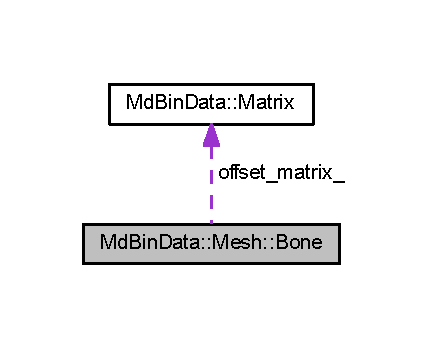
\includegraphics[width=206pt]{class_md_bin_data_1_1_mesh_1_1_bone__coll__graph}
\end{center}
\end{figure}
\subsection*{公開メンバ関数}
\begin{DoxyCompactItemize}
\item 
std\+::string $\ast$ \mbox{\hyperlink{class_md_bin_data_1_1_mesh_1_1_bone_a7a132ac01755ee4a6bca3c25ad3da42c}{getp\+Name}} ()
\begin{DoxyCompactList}\small\item\em ボーン名取得関数 \end{DoxyCompactList}\item 
\mbox{\hyperlink{class_md_bin_data_1_1_matrix}{Matrix}} $\ast$ \mbox{\hyperlink{class_md_bin_data_1_1_mesh_1_1_bone_a0e5d6012c7efa481bbb40cc86b8a0856}{getp\+Offset\+Matrix}} ()
\begin{DoxyCompactList}\small\item\em オフセット行列取得関数 \end{DoxyCompactList}\item 
int \mbox{\hyperlink{class_md_bin_data_1_1_mesh_1_1_bone_ad59efa7e03e444dabbdfef7848091ab9}{get\+Animation\+Matrix\+Array\+Size}} ()
\begin{DoxyCompactList}\small\item\em アニメーション行列配列サイズ取得関数 \end{DoxyCompactList}\item 
void \mbox{\hyperlink{class_md_bin_data_1_1_mesh_1_1_bone_af7edfd3047be8f110d4ab995738c6af3}{set\+Animation\+Matrix\+Array\+Size}} (int value)
\begin{DoxyCompactList}\small\item\em アニメーション行列配列サイズ設定関数 \end{DoxyCompactList}\item 
\mbox{\hyperlink{class_md_bin_data_1_1_matrix}{Matrix}} $\ast$ \mbox{\hyperlink{class_md_bin_data_1_1_mesh_1_1_bone_ac185537ff78d9e8e78c7d6845425f615}{getp\+Animation\+Matrix}} (int index)
\begin{DoxyCompactList}\small\item\em アニメーション行列取得関数 \end{DoxyCompactList}\end{DoxyCompactItemize}
\subsection*{非公開メンバ関数}
\begin{DoxyCompactItemize}
\item 
{\footnotesize template$<$class Archive $>$ }\\void \mbox{\hyperlink{class_md_bin_data_1_1_mesh_1_1_bone_aa28ecffb26fc5ae631664ae97c099a25}{serialize}} (Archive \&archive, const unsigned version)
\end{DoxyCompactItemize}
\subsection*{非公開変数類}
\begin{DoxyCompactItemize}
\item 
std\+::string \mbox{\hyperlink{class_md_bin_data_1_1_mesh_1_1_bone_a3ed12325ffa278847429e758ec08a373}{name\+\_\+}}
\begin{DoxyCompactList}\small\item\em ボーン名 \end{DoxyCompactList}\item 
\mbox{\hyperlink{class_md_bin_data_1_1_matrix}{Matrix}} \mbox{\hyperlink{class_md_bin_data_1_1_mesh_1_1_bone_ab2119901317e2beb384a36d40f31c385}{offset\+\_\+matrix\+\_\+}}
\begin{DoxyCompactList}\small\item\em オフセット行列(初期姿勢の逆行列) \end{DoxyCompactList}\item 
std\+::vector$<$ \mbox{\hyperlink{class_md_bin_data_1_1_matrix}{Matrix}} $>$ \mbox{\hyperlink{class_md_bin_data_1_1_mesh_1_1_bone_a434b2abeb02434b44881e07a0eb7002e}{animation\+\_\+matrix\+\_\+array\+\_\+}}
\begin{DoxyCompactList}\small\item\em アニメーション行列 \end{DoxyCompactList}\end{DoxyCompactItemize}
\subsection*{フレンド}
\begin{DoxyCompactItemize}
\item 
class \mbox{\hyperlink{class_md_bin_data_1_1_mesh_1_1_bone_ac98d07dd8f7b70e16ccb9a01abf56b9c}{boost\+::serialization\+::access}}
\begin{DoxyCompactList}\small\item\em シリアライズ(I/O)関数 \end{DoxyCompactList}\end{DoxyCompactItemize}


\subsection{詳解}
ボーン\+Class 

ボーンの\+Class 

 Md\+Bin\+Data.\+h の 664 行目に定義があります。



\subsection{関数詳解}
\mbox{\Hypertarget{class_md_bin_data_1_1_mesh_1_1_bone_ad59efa7e03e444dabbdfef7848091ab9}\label{class_md_bin_data_1_1_mesh_1_1_bone_ad59efa7e03e444dabbdfef7848091ab9}} 
\index{Md\+Bin\+Data\+::\+Mesh\+::\+Bone@{Md\+Bin\+Data\+::\+Mesh\+::\+Bone}!get\+Animation\+Matrix\+Array\+Size@{get\+Animation\+Matrix\+Array\+Size}}
\index{get\+Animation\+Matrix\+Array\+Size@{get\+Animation\+Matrix\+Array\+Size}!Md\+Bin\+Data\+::\+Mesh\+::\+Bone@{Md\+Bin\+Data\+::\+Mesh\+::\+Bone}}
\subsubsection{\texorpdfstring{get\+Animation\+Matrix\+Array\+Size()}{getAnimationMatrixArraySize()}}
{\footnotesize\ttfamily int Md\+Bin\+Data\+::\+Mesh\+::\+Bone\+::get\+Animation\+Matrix\+Array\+Size (\begin{DoxyParamCaption}{ }\end{DoxyParamCaption})}



アニメーション行列配列サイズ取得関数 


\begin{DoxyParams}{引数}
{\em void} & なし \\
\hline
\end{DoxyParams}

\begin{DoxyRetVals}{戻り値}
{\em int} & アニメーション行列配列サイズ \\
\hline
\end{DoxyRetVals}


 Md\+Bin\+Data.\+cpp の 278 行目に定義があります。

\mbox{\Hypertarget{class_md_bin_data_1_1_mesh_1_1_bone_ac185537ff78d9e8e78c7d6845425f615}\label{class_md_bin_data_1_1_mesh_1_1_bone_ac185537ff78d9e8e78c7d6845425f615}} 
\index{Md\+Bin\+Data\+::\+Mesh\+::\+Bone@{Md\+Bin\+Data\+::\+Mesh\+::\+Bone}!getp\+Animation\+Matrix@{getp\+Animation\+Matrix}}
\index{getp\+Animation\+Matrix@{getp\+Animation\+Matrix}!Md\+Bin\+Data\+::\+Mesh\+::\+Bone@{Md\+Bin\+Data\+::\+Mesh\+::\+Bone}}
\subsubsection{\texorpdfstring{getp\+Animation\+Matrix()}{getpAnimationMatrix()}}
{\footnotesize\ttfamily \mbox{\hyperlink{class_md_bin_data_1_1_matrix}{Md\+Bin\+Data\+::\+Matrix}} $\ast$ Md\+Bin\+Data\+::\+Mesh\+::\+Bone\+::getp\+Animation\+Matrix (\begin{DoxyParamCaption}\item[{int}]{index }\end{DoxyParamCaption})}



アニメーション行列取得関数 


\begin{DoxyParams}{引数}
{\em index} & インデックス \\
\hline
\end{DoxyParams}

\begin{DoxyRetVals}{戻り値}
{\em Matrix$\ast$} & アニメーション行列 \\
\hline
\end{DoxyRetVals}


 Md\+Bin\+Data.\+cpp の 292 行目に定義があります。

\mbox{\Hypertarget{class_md_bin_data_1_1_mesh_1_1_bone_a7a132ac01755ee4a6bca3c25ad3da42c}\label{class_md_bin_data_1_1_mesh_1_1_bone_a7a132ac01755ee4a6bca3c25ad3da42c}} 
\index{Md\+Bin\+Data\+::\+Mesh\+::\+Bone@{Md\+Bin\+Data\+::\+Mesh\+::\+Bone}!getp\+Name@{getp\+Name}}
\index{getp\+Name@{getp\+Name}!Md\+Bin\+Data\+::\+Mesh\+::\+Bone@{Md\+Bin\+Data\+::\+Mesh\+::\+Bone}}
\subsubsection{\texorpdfstring{getp\+Name()}{getpName()}}
{\footnotesize\ttfamily std\+::string $\ast$ Md\+Bin\+Data\+::\+Mesh\+::\+Bone\+::getp\+Name (\begin{DoxyParamCaption}{ }\end{DoxyParamCaption})}



ボーン名取得関数 


\begin{DoxyParams}{引数}
{\em void} & なし \\
\hline
\end{DoxyParams}

\begin{DoxyRetVals}{戻り値}
{\em std\+::string$\ast$} & ボーン名 \\
\hline
\end{DoxyRetVals}


 Md\+Bin\+Data.\+cpp の 264 行目に定義があります。

\mbox{\Hypertarget{class_md_bin_data_1_1_mesh_1_1_bone_a0e5d6012c7efa481bbb40cc86b8a0856}\label{class_md_bin_data_1_1_mesh_1_1_bone_a0e5d6012c7efa481bbb40cc86b8a0856}} 
\index{Md\+Bin\+Data\+::\+Mesh\+::\+Bone@{Md\+Bin\+Data\+::\+Mesh\+::\+Bone}!getp\+Offset\+Matrix@{getp\+Offset\+Matrix}}
\index{getp\+Offset\+Matrix@{getp\+Offset\+Matrix}!Md\+Bin\+Data\+::\+Mesh\+::\+Bone@{Md\+Bin\+Data\+::\+Mesh\+::\+Bone}}
\subsubsection{\texorpdfstring{getp\+Offset\+Matrix()}{getpOffsetMatrix()}}
{\footnotesize\ttfamily \mbox{\hyperlink{class_md_bin_data_1_1_matrix}{Md\+Bin\+Data\+::\+Matrix}} $\ast$ Md\+Bin\+Data\+::\+Mesh\+::\+Bone\+::getp\+Offset\+Matrix (\begin{DoxyParamCaption}{ }\end{DoxyParamCaption})}



オフセット行列取得関数 


\begin{DoxyParams}{引数}
{\em void} & なし \\
\hline
\end{DoxyParams}

\begin{DoxyRetVals}{戻り値}
{\em Matirx$\ast$} & オフセット配列 \\
\hline
\end{DoxyRetVals}


 Md\+Bin\+Data.\+cpp の 271 行目に定義があります。

\mbox{\Hypertarget{class_md_bin_data_1_1_mesh_1_1_bone_aa28ecffb26fc5ae631664ae97c099a25}\label{class_md_bin_data_1_1_mesh_1_1_bone_aa28ecffb26fc5ae631664ae97c099a25}} 
\index{Md\+Bin\+Data\+::\+Mesh\+::\+Bone@{Md\+Bin\+Data\+::\+Mesh\+::\+Bone}!serialize@{serialize}}
\index{serialize@{serialize}!Md\+Bin\+Data\+::\+Mesh\+::\+Bone@{Md\+Bin\+Data\+::\+Mesh\+::\+Bone}}
\subsubsection{\texorpdfstring{serialize()}{serialize()}}
{\footnotesize\ttfamily template$<$class Archive $>$ \\
void Md\+Bin\+Data\+::\+Mesh\+::\+Bone\+::serialize (\begin{DoxyParamCaption}\item[{Archive \&}]{archive,  }\item[{const unsigned}]{version }\end{DoxyParamCaption})\hspace{0.3cm}{\ttfamily [inline]}, {\ttfamily [private]}}



 Md\+Bin\+Data.\+h の 733 行目に定義があります。

\mbox{\Hypertarget{class_md_bin_data_1_1_mesh_1_1_bone_af7edfd3047be8f110d4ab995738c6af3}\label{class_md_bin_data_1_1_mesh_1_1_bone_af7edfd3047be8f110d4ab995738c6af3}} 
\index{Md\+Bin\+Data\+::\+Mesh\+::\+Bone@{Md\+Bin\+Data\+::\+Mesh\+::\+Bone}!set\+Animation\+Matrix\+Array\+Size@{set\+Animation\+Matrix\+Array\+Size}}
\index{set\+Animation\+Matrix\+Array\+Size@{set\+Animation\+Matrix\+Array\+Size}!Md\+Bin\+Data\+::\+Mesh\+::\+Bone@{Md\+Bin\+Data\+::\+Mesh\+::\+Bone}}
\subsubsection{\texorpdfstring{set\+Animation\+Matrix\+Array\+Size()}{setAnimationMatrixArraySize()}}
{\footnotesize\ttfamily void Md\+Bin\+Data\+::\+Mesh\+::\+Bone\+::set\+Animation\+Matrix\+Array\+Size (\begin{DoxyParamCaption}\item[{int}]{value }\end{DoxyParamCaption})}



アニメーション行列配列サイズ設定関数 


\begin{DoxyParams}{引数}
{\em value} & アニメーション行列配列サイズ \\
\hline
\end{DoxyParams}

\begin{DoxyRetVals}{戻り値}
{\em void} & なし \\
\hline
\end{DoxyRetVals}


 Md\+Bin\+Data.\+cpp の 285 行目に定義があります。



\subsection{フレンドと関連関数の詳解}
\mbox{\Hypertarget{class_md_bin_data_1_1_mesh_1_1_bone_ac98d07dd8f7b70e16ccb9a01abf56b9c}\label{class_md_bin_data_1_1_mesh_1_1_bone_ac98d07dd8f7b70e16ccb9a01abf56b9c}} 
\index{Md\+Bin\+Data\+::\+Mesh\+::\+Bone@{Md\+Bin\+Data\+::\+Mesh\+::\+Bone}!boost\+::serialization\+::access@{boost\+::serialization\+::access}}
\index{boost\+::serialization\+::access@{boost\+::serialization\+::access}!Md\+Bin\+Data\+::\+Mesh\+::\+Bone@{Md\+Bin\+Data\+::\+Mesh\+::\+Bone}}
\subsubsection{\texorpdfstring{boost\+::serialization\+::access}{boost::serialization::access}}
{\footnotesize\ttfamily friend class boost\+::serialization\+::access\hspace{0.3cm}{\ttfamily [friend]}}



シリアライズ(I/O)関数 


\begin{DoxyParams}{引数}
{\em archive} & アーカイブ用クラス \\
\hline
{\em version} & バージョン \\
\hline
\end{DoxyParams}

\begin{DoxyRetVals}{戻り値}
{\em void} & なし \\
\hline
\end{DoxyRetVals}


 Md\+Bin\+Data.\+h の 731 行目に定義があります。



\subsection{メンバ詳解}
\mbox{\Hypertarget{class_md_bin_data_1_1_mesh_1_1_bone_a434b2abeb02434b44881e07a0eb7002e}\label{class_md_bin_data_1_1_mesh_1_1_bone_a434b2abeb02434b44881e07a0eb7002e}} 
\index{Md\+Bin\+Data\+::\+Mesh\+::\+Bone@{Md\+Bin\+Data\+::\+Mesh\+::\+Bone}!animation\+\_\+matrix\+\_\+array\+\_\+@{animation\+\_\+matrix\+\_\+array\+\_\+}}
\index{animation\+\_\+matrix\+\_\+array\+\_\+@{animation\+\_\+matrix\+\_\+array\+\_\+}!Md\+Bin\+Data\+::\+Mesh\+::\+Bone@{Md\+Bin\+Data\+::\+Mesh\+::\+Bone}}
\subsubsection{\texorpdfstring{animation\+\_\+matrix\+\_\+array\+\_\+}{animation\_matrix\_array\_}}
{\footnotesize\ttfamily std\+::vector$<$\mbox{\hyperlink{class_md_bin_data_1_1_matrix}{Matrix}}$>$ Md\+Bin\+Data\+::\+Mesh\+::\+Bone\+::animation\+\_\+matrix\+\_\+array\+\_\+\hspace{0.3cm}{\ttfamily [private]}}



アニメーション行列 



 Md\+Bin\+Data.\+h の 672 行目に定義があります。

\mbox{\Hypertarget{class_md_bin_data_1_1_mesh_1_1_bone_a3ed12325ffa278847429e758ec08a373}\label{class_md_bin_data_1_1_mesh_1_1_bone_a3ed12325ffa278847429e758ec08a373}} 
\index{Md\+Bin\+Data\+::\+Mesh\+::\+Bone@{Md\+Bin\+Data\+::\+Mesh\+::\+Bone}!name\+\_\+@{name\+\_\+}}
\index{name\+\_\+@{name\+\_\+}!Md\+Bin\+Data\+::\+Mesh\+::\+Bone@{Md\+Bin\+Data\+::\+Mesh\+::\+Bone}}
\subsubsection{\texorpdfstring{name\+\_\+}{name\_}}
{\footnotesize\ttfamily std\+::string Md\+Bin\+Data\+::\+Mesh\+::\+Bone\+::name\+\_\+\hspace{0.3cm}{\ttfamily [private]}}



ボーン名 



 Md\+Bin\+Data.\+h の 670 行目に定義があります。

\mbox{\Hypertarget{class_md_bin_data_1_1_mesh_1_1_bone_ab2119901317e2beb384a36d40f31c385}\label{class_md_bin_data_1_1_mesh_1_1_bone_ab2119901317e2beb384a36d40f31c385}} 
\index{Md\+Bin\+Data\+::\+Mesh\+::\+Bone@{Md\+Bin\+Data\+::\+Mesh\+::\+Bone}!offset\+\_\+matrix\+\_\+@{offset\+\_\+matrix\+\_\+}}
\index{offset\+\_\+matrix\+\_\+@{offset\+\_\+matrix\+\_\+}!Md\+Bin\+Data\+::\+Mesh\+::\+Bone@{Md\+Bin\+Data\+::\+Mesh\+::\+Bone}}
\subsubsection{\texorpdfstring{offset\+\_\+matrix\+\_\+}{offset\_matrix\_}}
{\footnotesize\ttfamily \mbox{\hyperlink{class_md_bin_data_1_1_matrix}{Matrix}} Md\+Bin\+Data\+::\+Mesh\+::\+Bone\+::offset\+\_\+matrix\+\_\+\hspace{0.3cm}{\ttfamily [private]}}



オフセット行列(初期姿勢の逆行列) 



 Md\+Bin\+Data.\+h の 671 行目に定義があります。



このクラス詳解は次のファイルから抽出されました\+:\begin{DoxyCompactItemize}
\item 
C\+:/\+H\+A\+L/\+P\+G関係/03\+\_\+作成プログラム/03\+\_\+\+H\+A\+L授業/就職作品/\+Fbx\+Converter/source/\+Md\+Bin\+Data/\mbox{\hyperlink{_md_bin_data_8h}{Md\+Bin\+Data.\+h}}\item 
C\+:/\+H\+A\+L/\+P\+G関係/03\+\_\+作成プログラム/03\+\_\+\+H\+A\+L授業/就職作品/\+Fbx\+Converter/source/\+Md\+Bin\+Data/\mbox{\hyperlink{_md_bin_data_8cpp}{Md\+Bin\+Data.\+cpp}}\end{DoxyCompactItemize}

\hypertarget{class_md_bin_data_1_1_mesh_1_1_bone_weight}{}\section{Md\+Bin\+Data\+:\+:Mesh\+:\+:Bone\+Weight クラス}
\label{class_md_bin_data_1_1_mesh_1_1_bone_weight}\index{Md\+Bin\+Data\+::\+Mesh\+::\+Bone\+Weight@{Md\+Bin\+Data\+::\+Mesh\+::\+Bone\+Weight}}


ボーン重み\+Class  




{\ttfamily \#include $<$Md\+Bin\+Data.\+h$>$}

\subsection*{公開メンバ関数}
\begin{DoxyCompactItemize}
\item 
int \mbox{\hyperlink{class_md_bin_data_1_1_mesh_1_1_bone_weight_a0e88a654cd1a709780357cb5c612070e}{get\+Bone\+Index}} (int index)
\begin{DoxyCompactList}\small\item\em ボーンインデックス取得関数 \end{DoxyCompactList}\item 
float \mbox{\hyperlink{class_md_bin_data_1_1_mesh_1_1_bone_weight_a3beb8b0ee437d812fe8c0cccd6acb194}{get\+Bone\+Weight}} (int index)
\begin{DoxyCompactList}\small\item\em ボーンの重み取得関数 \end{DoxyCompactList}\item 
void \mbox{\hyperlink{class_md_bin_data_1_1_mesh_1_1_bone_weight_a219857a3874c416784d461366e867d57}{set\+Bone\+Index\+And\+Weight}} (int bone\+\_\+index, float bone\+\_\+weight)
\begin{DoxyCompactList}\small\item\em ボーンインデックス\&重み設定関数 \end{DoxyCompactList}\item 
void \mbox{\hyperlink{class_md_bin_data_1_1_mesh_1_1_bone_weight_a01430f0a589f6276dffeab831c573708}{Init}} ()
\begin{DoxyCompactList}\small\item\em 初期化関数 \end{DoxyCompactList}\end{DoxyCompactItemize}
\subsection*{静的公開変数類}
\begin{DoxyCompactItemize}
\item 
static const unsigned \mbox{\hyperlink{class_md_bin_data_1_1_mesh_1_1_bone_weight_a2c870f6c96315b6b9630cff3c24b79e7}{M\+A\+X\+\_\+\+B\+O\+N\+E\+\_\+\+N\+UM}} = 4
\begin{DoxyCompactList}\small\item\em 最大ボーン数 \end{DoxyCompactList}\end{DoxyCompactItemize}
\subsection*{非公開メンバ関数}
\begin{DoxyCompactItemize}
\item 
{\footnotesize template$<$class Archive $>$ }\\void \mbox{\hyperlink{class_md_bin_data_1_1_mesh_1_1_bone_weight_a2ffaf506ea648dc122ff380eb9f81010}{serialize}} (Archive \&archive, const unsigned version)
\end{DoxyCompactItemize}
\subsection*{非公開変数類}
\begin{DoxyCompactItemize}
\item 
int \mbox{\hyperlink{class_md_bin_data_1_1_mesh_1_1_bone_weight_acfd3a3787786ddce83e1360d4c66dc4e}{bone\+\_\+index\+\_\+}} \mbox{[}\mbox{\hyperlink{class_md_bin_data_1_1_mesh_1_1_bone_weight_a2c870f6c96315b6b9630cff3c24b79e7}{M\+A\+X\+\_\+\+B\+O\+N\+E\+\_\+\+N\+UM}}\mbox{]}
\begin{DoxyCompactList}\small\item\em ボーンインデックス \end{DoxyCompactList}\item 
float \mbox{\hyperlink{class_md_bin_data_1_1_mesh_1_1_bone_weight_a0122907a7aa6c928e0a14e6e577e4b80}{bone\+\_\+weight\+\_\+}} \mbox{[}\mbox{\hyperlink{class_md_bin_data_1_1_mesh_1_1_bone_weight_a2c870f6c96315b6b9630cff3c24b79e7}{M\+A\+X\+\_\+\+B\+O\+N\+E\+\_\+\+N\+UM}}\mbox{]}
\begin{DoxyCompactList}\small\item\em ボーンの重み \end{DoxyCompactList}\end{DoxyCompactItemize}
\subsection*{フレンド}
\begin{DoxyCompactItemize}
\item 
class \mbox{\hyperlink{class_md_bin_data_1_1_mesh_1_1_bone_weight_ac98d07dd8f7b70e16ccb9a01abf56b9c}{boost\+::serialization\+::access}}
\begin{DoxyCompactList}\small\item\em シリアライズ(I/O)関数 \end{DoxyCompactList}\end{DoxyCompactItemize}


\subsection{詳解}
ボーン重み\+Class 

ボーンの重み\+Class 

 Md\+Bin\+Data.\+h の 749 行目に定義があります。



\subsection{関数詳解}
\mbox{\Hypertarget{class_md_bin_data_1_1_mesh_1_1_bone_weight_a0e88a654cd1a709780357cb5c612070e}\label{class_md_bin_data_1_1_mesh_1_1_bone_weight_a0e88a654cd1a709780357cb5c612070e}} 
\index{Md\+Bin\+Data\+::\+Mesh\+::\+Bone\+Weight@{Md\+Bin\+Data\+::\+Mesh\+::\+Bone\+Weight}!get\+Bone\+Index@{get\+Bone\+Index}}
\index{get\+Bone\+Index@{get\+Bone\+Index}!Md\+Bin\+Data\+::\+Mesh\+::\+Bone\+Weight@{Md\+Bin\+Data\+::\+Mesh\+::\+Bone\+Weight}}
\subsubsection{\texorpdfstring{get\+Bone\+Index()}{getBoneIndex()}}
{\footnotesize\ttfamily int Md\+Bin\+Data\+::\+Mesh\+::\+Bone\+Weight\+::get\+Bone\+Index (\begin{DoxyParamCaption}\item[{int}]{index }\end{DoxyParamCaption})}



ボーンインデックス取得関数 


\begin{DoxyParams}{引数}
{\em index} & インデックス \\
\hline
\end{DoxyParams}

\begin{DoxyRetVals}{戻り値}
{\em int} & ボーンインデックス \\
\hline
\end{DoxyRetVals}


 Md\+Bin\+Data.\+cpp の 299 行目に定義があります。

\mbox{\Hypertarget{class_md_bin_data_1_1_mesh_1_1_bone_weight_a3beb8b0ee437d812fe8c0cccd6acb194}\label{class_md_bin_data_1_1_mesh_1_1_bone_weight_a3beb8b0ee437d812fe8c0cccd6acb194}} 
\index{Md\+Bin\+Data\+::\+Mesh\+::\+Bone\+Weight@{Md\+Bin\+Data\+::\+Mesh\+::\+Bone\+Weight}!get\+Bone\+Weight@{get\+Bone\+Weight}}
\index{get\+Bone\+Weight@{get\+Bone\+Weight}!Md\+Bin\+Data\+::\+Mesh\+::\+Bone\+Weight@{Md\+Bin\+Data\+::\+Mesh\+::\+Bone\+Weight}}
\subsubsection{\texorpdfstring{get\+Bone\+Weight()}{getBoneWeight()}}
{\footnotesize\ttfamily float Md\+Bin\+Data\+::\+Mesh\+::\+Bone\+Weight\+::get\+Bone\+Weight (\begin{DoxyParamCaption}\item[{int}]{index }\end{DoxyParamCaption})}



ボーンの重み取得関数 


\begin{DoxyParams}{引数}
{\em index} & インデックス \\
\hline
\end{DoxyParams}

\begin{DoxyRetVals}{戻り値}
{\em float} & ボーンの重み \\
\hline
\end{DoxyRetVals}


 Md\+Bin\+Data.\+cpp の 306 行目に定義があります。

\mbox{\Hypertarget{class_md_bin_data_1_1_mesh_1_1_bone_weight_a01430f0a589f6276dffeab831c573708}\label{class_md_bin_data_1_1_mesh_1_1_bone_weight_a01430f0a589f6276dffeab831c573708}} 
\index{Md\+Bin\+Data\+::\+Mesh\+::\+Bone\+Weight@{Md\+Bin\+Data\+::\+Mesh\+::\+Bone\+Weight}!Init@{Init}}
\index{Init@{Init}!Md\+Bin\+Data\+::\+Mesh\+::\+Bone\+Weight@{Md\+Bin\+Data\+::\+Mesh\+::\+Bone\+Weight}}
\subsubsection{\texorpdfstring{Init()}{Init()}}
{\footnotesize\ttfamily void Md\+Bin\+Data\+::\+Mesh\+::\+Bone\+Weight\+::\+Init (\begin{DoxyParamCaption}{ }\end{DoxyParamCaption})}



初期化関数 


\begin{DoxyParams}{引数}
{\em void} & なし \\
\hline
\end{DoxyParams}

\begin{DoxyRetVals}{戻り値}
{\em void} & なし \\
\hline
\end{DoxyRetVals}


 Md\+Bin\+Data.\+cpp の 566 行目に定義があります。

\mbox{\Hypertarget{class_md_bin_data_1_1_mesh_1_1_bone_weight_a2ffaf506ea648dc122ff380eb9f81010}\label{class_md_bin_data_1_1_mesh_1_1_bone_weight_a2ffaf506ea648dc122ff380eb9f81010}} 
\index{Md\+Bin\+Data\+::\+Mesh\+::\+Bone\+Weight@{Md\+Bin\+Data\+::\+Mesh\+::\+Bone\+Weight}!serialize@{serialize}}
\index{serialize@{serialize}!Md\+Bin\+Data\+::\+Mesh\+::\+Bone\+Weight@{Md\+Bin\+Data\+::\+Mesh\+::\+Bone\+Weight}}
\subsubsection{\texorpdfstring{serialize()}{serialize()}}
{\footnotesize\ttfamily template$<$class Archive $>$ \\
void Md\+Bin\+Data\+::\+Mesh\+::\+Bone\+Weight\+::serialize (\begin{DoxyParamCaption}\item[{Archive \&}]{archive,  }\item[{const unsigned}]{version }\end{DoxyParamCaption})\hspace{0.3cm}{\ttfamily [inline]}, {\ttfamily [private]}}



 Md\+Bin\+Data.\+h の 822 行目に定義があります。

\mbox{\Hypertarget{class_md_bin_data_1_1_mesh_1_1_bone_weight_a219857a3874c416784d461366e867d57}\label{class_md_bin_data_1_1_mesh_1_1_bone_weight_a219857a3874c416784d461366e867d57}} 
\index{Md\+Bin\+Data\+::\+Mesh\+::\+Bone\+Weight@{Md\+Bin\+Data\+::\+Mesh\+::\+Bone\+Weight}!set\+Bone\+Index\+And\+Weight@{set\+Bone\+Index\+And\+Weight}}
\index{set\+Bone\+Index\+And\+Weight@{set\+Bone\+Index\+And\+Weight}!Md\+Bin\+Data\+::\+Mesh\+::\+Bone\+Weight@{Md\+Bin\+Data\+::\+Mesh\+::\+Bone\+Weight}}
\subsubsection{\texorpdfstring{set\+Bone\+Index\+And\+Weight()}{setBoneIndexAndWeight()}}
{\footnotesize\ttfamily void Md\+Bin\+Data\+::\+Mesh\+::\+Bone\+Weight\+::set\+Bone\+Index\+And\+Weight (\begin{DoxyParamCaption}\item[{int}]{bone\+\_\+index,  }\item[{float}]{bone\+\_\+weight }\end{DoxyParamCaption})}



ボーンインデックス\&重み設定関数 


\begin{DoxyParams}{引数}
{\em bone\+\_\+index} & ボーンインデックス \\
\hline
{\em bone\+\_\+weight} & ボーンの重み \\
\hline
\end{DoxyParams}

\begin{DoxyRetVals}{戻り値}
{\em int$\ast$} & ボーンインデックス \\
\hline
\end{DoxyRetVals}


 Md\+Bin\+Data.\+cpp の 313 行目に定義があります。



\subsection{フレンドと関連関数の詳解}
\mbox{\Hypertarget{class_md_bin_data_1_1_mesh_1_1_bone_weight_ac98d07dd8f7b70e16ccb9a01abf56b9c}\label{class_md_bin_data_1_1_mesh_1_1_bone_weight_ac98d07dd8f7b70e16ccb9a01abf56b9c}} 
\index{Md\+Bin\+Data\+::\+Mesh\+::\+Bone\+Weight@{Md\+Bin\+Data\+::\+Mesh\+::\+Bone\+Weight}!boost\+::serialization\+::access@{boost\+::serialization\+::access}}
\index{boost\+::serialization\+::access@{boost\+::serialization\+::access}!Md\+Bin\+Data\+::\+Mesh\+::\+Bone\+Weight@{Md\+Bin\+Data\+::\+Mesh\+::\+Bone\+Weight}}
\subsubsection{\texorpdfstring{boost\+::serialization\+::access}{boost::serialization::access}}
{\footnotesize\ttfamily friend class boost\+::serialization\+::access\hspace{0.3cm}{\ttfamily [friend]}}



シリアライズ(I/O)関数 


\begin{DoxyParams}{引数}
{\em archive} & アーカイブ用クラス \\
\hline
{\em version} & バージョン \\
\hline
\end{DoxyParams}

\begin{DoxyRetVals}{戻り値}
{\em void} & なし \\
\hline
\end{DoxyRetVals}


 Md\+Bin\+Data.\+h の 820 行目に定義があります。



\subsection{メンバ詳解}
\mbox{\Hypertarget{class_md_bin_data_1_1_mesh_1_1_bone_weight_acfd3a3787786ddce83e1360d4c66dc4e}\label{class_md_bin_data_1_1_mesh_1_1_bone_weight_acfd3a3787786ddce83e1360d4c66dc4e}} 
\index{Md\+Bin\+Data\+::\+Mesh\+::\+Bone\+Weight@{Md\+Bin\+Data\+::\+Mesh\+::\+Bone\+Weight}!bone\+\_\+index\+\_\+@{bone\+\_\+index\+\_\+}}
\index{bone\+\_\+index\+\_\+@{bone\+\_\+index\+\_\+}!Md\+Bin\+Data\+::\+Mesh\+::\+Bone\+Weight@{Md\+Bin\+Data\+::\+Mesh\+::\+Bone\+Weight}}
\subsubsection{\texorpdfstring{bone\+\_\+index\+\_\+}{bone\_index\_}}
{\footnotesize\ttfamily int Md\+Bin\+Data\+::\+Mesh\+::\+Bone\+Weight\+::bone\+\_\+index\+\_\+\mbox{[}\mbox{\hyperlink{class_md_bin_data_1_1_mesh_1_1_bone_weight_a2c870f6c96315b6b9630cff3c24b79e7}{M\+A\+X\+\_\+\+B\+O\+N\+E\+\_\+\+N\+UM}}\mbox{]}\hspace{0.3cm}{\ttfamily [private]}}



ボーンインデックス 



 Md\+Bin\+Data.\+h の 762 行目に定義があります。

\mbox{\Hypertarget{class_md_bin_data_1_1_mesh_1_1_bone_weight_a0122907a7aa6c928e0a14e6e577e4b80}\label{class_md_bin_data_1_1_mesh_1_1_bone_weight_a0122907a7aa6c928e0a14e6e577e4b80}} 
\index{Md\+Bin\+Data\+::\+Mesh\+::\+Bone\+Weight@{Md\+Bin\+Data\+::\+Mesh\+::\+Bone\+Weight}!bone\+\_\+weight\+\_\+@{bone\+\_\+weight\+\_\+}}
\index{bone\+\_\+weight\+\_\+@{bone\+\_\+weight\+\_\+}!Md\+Bin\+Data\+::\+Mesh\+::\+Bone\+Weight@{Md\+Bin\+Data\+::\+Mesh\+::\+Bone\+Weight}}
\subsubsection{\texorpdfstring{bone\+\_\+weight\+\_\+}{bone\_weight\_}}
{\footnotesize\ttfamily float Md\+Bin\+Data\+::\+Mesh\+::\+Bone\+Weight\+::bone\+\_\+weight\+\_\+\mbox{[}\mbox{\hyperlink{class_md_bin_data_1_1_mesh_1_1_bone_weight_a2c870f6c96315b6b9630cff3c24b79e7}{M\+A\+X\+\_\+\+B\+O\+N\+E\+\_\+\+N\+UM}}\mbox{]}\hspace{0.3cm}{\ttfamily [private]}}



ボーンの重み 



 Md\+Bin\+Data.\+h の 763 行目に定義があります。

\mbox{\Hypertarget{class_md_bin_data_1_1_mesh_1_1_bone_weight_a2c870f6c96315b6b9630cff3c24b79e7}\label{class_md_bin_data_1_1_mesh_1_1_bone_weight_a2c870f6c96315b6b9630cff3c24b79e7}} 
\index{Md\+Bin\+Data\+::\+Mesh\+::\+Bone\+Weight@{Md\+Bin\+Data\+::\+Mesh\+::\+Bone\+Weight}!M\+A\+X\+\_\+\+B\+O\+N\+E\+\_\+\+N\+UM@{M\+A\+X\+\_\+\+B\+O\+N\+E\+\_\+\+N\+UM}}
\index{M\+A\+X\+\_\+\+B\+O\+N\+E\+\_\+\+N\+UM@{M\+A\+X\+\_\+\+B\+O\+N\+E\+\_\+\+N\+UM}!Md\+Bin\+Data\+::\+Mesh\+::\+Bone\+Weight@{Md\+Bin\+Data\+::\+Mesh\+::\+Bone\+Weight}}
\subsubsection{\texorpdfstring{M\+A\+X\+\_\+\+B\+O\+N\+E\+\_\+\+N\+UM}{MAX\_BONE\_NUM}}
{\footnotesize\ttfamily const unsigned Md\+Bin\+Data\+::\+Mesh\+::\+Bone\+Weight\+::\+M\+A\+X\+\_\+\+B\+O\+N\+E\+\_\+\+N\+UM = 4\hspace{0.3cm}{\ttfamily [static]}}



最大ボーン数 



 Md\+Bin\+Data.\+h の 755 行目に定義があります。



このクラス詳解は次のファイルから抽出されました\+:\begin{DoxyCompactItemize}
\item 
C\+:/\+H\+A\+L/\+P\+G関係/03\+\_\+作成プログラム/03\+\_\+\+H\+A\+L授業/就職作品/\+Fbx\+Converter/source/\+Md\+Bin\+Data/\mbox{\hyperlink{_md_bin_data_8h}{Md\+Bin\+Data.\+h}}\item 
C\+:/\+H\+A\+L/\+P\+G関係/03\+\_\+作成プログラム/03\+\_\+\+H\+A\+L授業/就職作品/\+Fbx\+Converter/source/\+Md\+Bin\+Data/\mbox{\hyperlink{_md_bin_data_8cpp}{Md\+Bin\+Data.\+cpp}}\end{DoxyCompactItemize}

\hypertarget{class_md_bin_data_1_1_color}{}\section{Md\+Bin\+Data\+:\+:Color クラス}
\label{class_md_bin_data_1_1_color}\index{Md\+Bin\+Data\+::\+Color@{Md\+Bin\+Data\+::\+Color}}


色\+Class  




{\ttfamily \#include $<$Md\+Bin\+Data.\+h$>$}

\subsection*{公開メンバ関数}
\begin{DoxyCompactItemize}
\item 
float $\ast$ \mbox{\hyperlink{class_md_bin_data_1_1_color_aa4731175fd7438ff0e3d20db51fa87e2}{getpR}} ()
\begin{DoxyCompactList}\small\item\em 赤成分取得関数 \end{DoxyCompactList}\item 
float $\ast$ \mbox{\hyperlink{class_md_bin_data_1_1_color_a8d33bc92cef898d6026d8bd1f1fd51b0}{getpG}} ()
\begin{DoxyCompactList}\small\item\em 緑成分取得関数 \end{DoxyCompactList}\item 
float $\ast$ \mbox{\hyperlink{class_md_bin_data_1_1_color_adbd0c3f5aa7d8026e6d5638a4b42aeb6}{getpB}} ()
\begin{DoxyCompactList}\small\item\em 青成分取得関数 \end{DoxyCompactList}\end{DoxyCompactItemize}
\subsection*{非公開メンバ関数}
\begin{DoxyCompactItemize}
\item 
{\footnotesize template$<$class Archive $>$ }\\void \mbox{\hyperlink{class_md_bin_data_1_1_color_a7442aa5a639d3324010bb56f6db2a5fc}{serialize}} (Archive \&archive, const unsigned version)
\end{DoxyCompactItemize}
\subsection*{非公開変数類}
\begin{DoxyCompactItemize}
\item 
float \mbox{\hyperlink{class_md_bin_data_1_1_color_a86af984afebeabe57f5155c1981d9c94}{r\+\_\+}}
\begin{DoxyCompactList}\small\item\em 赤成分 \end{DoxyCompactList}\item 
float \mbox{\hyperlink{class_md_bin_data_1_1_color_a5bdd552987125758d30cbe395909b118}{g\+\_\+}}
\begin{DoxyCompactList}\small\item\em 緑成分 \end{DoxyCompactList}\item 
float \mbox{\hyperlink{class_md_bin_data_1_1_color_a082688900f611ea48822a5b4ccd74afc}{b\+\_\+}}
\begin{DoxyCompactList}\small\item\em 青成分 \end{DoxyCompactList}\end{DoxyCompactItemize}
\subsection*{フレンド}
\begin{DoxyCompactItemize}
\item 
class \mbox{\hyperlink{class_md_bin_data_1_1_color_ac98d07dd8f7b70e16ccb9a01abf56b9c}{boost\+::serialization\+::access}}
\begin{DoxyCompactList}\small\item\em シリアライズ(I/O)関数 \end{DoxyCompactList}\end{DoxyCompactItemize}


\subsection{詳解}
色\+Class 

色の\+Class 

 Md\+Bin\+Data.\+h の 165 行目に定義があります。



\subsection{関数詳解}
\mbox{\Hypertarget{class_md_bin_data_1_1_color_adbd0c3f5aa7d8026e6d5638a4b42aeb6}\label{class_md_bin_data_1_1_color_adbd0c3f5aa7d8026e6d5638a4b42aeb6}} 
\index{Md\+Bin\+Data\+::\+Color@{Md\+Bin\+Data\+::\+Color}!getpB@{getpB}}
\index{getpB@{getpB}!Md\+Bin\+Data\+::\+Color@{Md\+Bin\+Data\+::\+Color}}
\subsubsection{\texorpdfstring{getp\+B()}{getpB()}}
{\footnotesize\ttfamily float $\ast$ Md\+Bin\+Data\+::\+Color\+::getpB (\begin{DoxyParamCaption}{ }\end{DoxyParamCaption})}



青成分取得関数 


\begin{DoxyParams}{引数}
{\em void} & なし \\
\hline
\end{DoxyParams}

\begin{DoxyRetVals}{戻り値}
{\em float$\ast$} & 青成分 \\
\hline
\end{DoxyRetVals}


 Md\+Bin\+Data.\+cpp の 110 行目に定義があります。

\mbox{\Hypertarget{class_md_bin_data_1_1_color_a8d33bc92cef898d6026d8bd1f1fd51b0}\label{class_md_bin_data_1_1_color_a8d33bc92cef898d6026d8bd1f1fd51b0}} 
\index{Md\+Bin\+Data\+::\+Color@{Md\+Bin\+Data\+::\+Color}!getpG@{getpG}}
\index{getpG@{getpG}!Md\+Bin\+Data\+::\+Color@{Md\+Bin\+Data\+::\+Color}}
\subsubsection{\texorpdfstring{getp\+G()}{getpG()}}
{\footnotesize\ttfamily float $\ast$ Md\+Bin\+Data\+::\+Color\+::getpG (\begin{DoxyParamCaption}{ }\end{DoxyParamCaption})}



緑成分取得関数 


\begin{DoxyParams}{引数}
{\em void} & なし \\
\hline
\end{DoxyParams}

\begin{DoxyRetVals}{戻り値}
{\em float$\ast$} & 緑成分 \\
\hline
\end{DoxyRetVals}


 Md\+Bin\+Data.\+cpp の 103 行目に定義があります。

\mbox{\Hypertarget{class_md_bin_data_1_1_color_aa4731175fd7438ff0e3d20db51fa87e2}\label{class_md_bin_data_1_1_color_aa4731175fd7438ff0e3d20db51fa87e2}} 
\index{Md\+Bin\+Data\+::\+Color@{Md\+Bin\+Data\+::\+Color}!getpR@{getpR}}
\index{getpR@{getpR}!Md\+Bin\+Data\+::\+Color@{Md\+Bin\+Data\+::\+Color}}
\subsubsection{\texorpdfstring{getp\+R()}{getpR()}}
{\footnotesize\ttfamily float $\ast$ Md\+Bin\+Data\+::\+Color\+::getpR (\begin{DoxyParamCaption}{ }\end{DoxyParamCaption})}



赤成分取得関数 


\begin{DoxyParams}{引数}
{\em void} & なし \\
\hline
\end{DoxyParams}

\begin{DoxyRetVals}{戻り値}
{\em float$\ast$} & 赤成分 \\
\hline
\end{DoxyRetVals}


 Md\+Bin\+Data.\+cpp の 96 行目に定義があります。

\mbox{\Hypertarget{class_md_bin_data_1_1_color_a7442aa5a639d3324010bb56f6db2a5fc}\label{class_md_bin_data_1_1_color_a7442aa5a639d3324010bb56f6db2a5fc}} 
\index{Md\+Bin\+Data\+::\+Color@{Md\+Bin\+Data\+::\+Color}!serialize@{serialize}}
\index{serialize@{serialize}!Md\+Bin\+Data\+::\+Color@{Md\+Bin\+Data\+::\+Color}}
\subsubsection{\texorpdfstring{serialize()}{serialize()}}
{\footnotesize\ttfamily template$<$class Archive $>$ \\
void Md\+Bin\+Data\+::\+Color\+::serialize (\begin{DoxyParamCaption}\item[{Archive \&}]{archive,  }\item[{const unsigned}]{version }\end{DoxyParamCaption})\hspace{0.3cm}{\ttfamily [inline]}, {\ttfamily [private]}}



 Md\+Bin\+Data.\+h の 218 行目に定義があります。



\subsection{フレンドと関連関数の詳解}
\mbox{\Hypertarget{class_md_bin_data_1_1_color_ac98d07dd8f7b70e16ccb9a01abf56b9c}\label{class_md_bin_data_1_1_color_ac98d07dd8f7b70e16ccb9a01abf56b9c}} 
\index{Md\+Bin\+Data\+::\+Color@{Md\+Bin\+Data\+::\+Color}!boost\+::serialization\+::access@{boost\+::serialization\+::access}}
\index{boost\+::serialization\+::access@{boost\+::serialization\+::access}!Md\+Bin\+Data\+::\+Color@{Md\+Bin\+Data\+::\+Color}}
\subsubsection{\texorpdfstring{boost\+::serialization\+::access}{boost::serialization::access}}
{\footnotesize\ttfamily friend class boost\+::serialization\+::access\hspace{0.3cm}{\ttfamily [friend]}}



シリアライズ(I/O)関数 


\begin{DoxyParams}{引数}
{\em archive} & アーカイブ用クラス \\
\hline
{\em version} & バージョン \\
\hline
\end{DoxyParams}

\begin{DoxyRetVals}{戻り値}
{\em void} & なし \\
\hline
\end{DoxyRetVals}


 Md\+Bin\+Data.\+h の 216 行目に定義があります。



\subsection{メンバ詳解}
\mbox{\Hypertarget{class_md_bin_data_1_1_color_a082688900f611ea48822a5b4ccd74afc}\label{class_md_bin_data_1_1_color_a082688900f611ea48822a5b4ccd74afc}} 
\index{Md\+Bin\+Data\+::\+Color@{Md\+Bin\+Data\+::\+Color}!b\+\_\+@{b\+\_\+}}
\index{b\+\_\+@{b\+\_\+}!Md\+Bin\+Data\+::\+Color@{Md\+Bin\+Data\+::\+Color}}
\subsubsection{\texorpdfstring{b\+\_\+}{b\_}}
{\footnotesize\ttfamily float Md\+Bin\+Data\+::\+Color\+::b\+\_\+\hspace{0.3cm}{\ttfamily [private]}}



青成分 



 Md\+Bin\+Data.\+h の 173 行目に定義があります。

\mbox{\Hypertarget{class_md_bin_data_1_1_color_a5bdd552987125758d30cbe395909b118}\label{class_md_bin_data_1_1_color_a5bdd552987125758d30cbe395909b118}} 
\index{Md\+Bin\+Data\+::\+Color@{Md\+Bin\+Data\+::\+Color}!g\+\_\+@{g\+\_\+}}
\index{g\+\_\+@{g\+\_\+}!Md\+Bin\+Data\+::\+Color@{Md\+Bin\+Data\+::\+Color}}
\subsubsection{\texorpdfstring{g\+\_\+}{g\_}}
{\footnotesize\ttfamily float Md\+Bin\+Data\+::\+Color\+::g\+\_\+\hspace{0.3cm}{\ttfamily [private]}}



緑成分 



 Md\+Bin\+Data.\+h の 172 行目に定義があります。

\mbox{\Hypertarget{class_md_bin_data_1_1_color_a86af984afebeabe57f5155c1981d9c94}\label{class_md_bin_data_1_1_color_a86af984afebeabe57f5155c1981d9c94}} 
\index{Md\+Bin\+Data\+::\+Color@{Md\+Bin\+Data\+::\+Color}!r\+\_\+@{r\+\_\+}}
\index{r\+\_\+@{r\+\_\+}!Md\+Bin\+Data\+::\+Color@{Md\+Bin\+Data\+::\+Color}}
\subsubsection{\texorpdfstring{r\+\_\+}{r\_}}
{\footnotesize\ttfamily float Md\+Bin\+Data\+::\+Color\+::r\+\_\+\hspace{0.3cm}{\ttfamily [private]}}



赤成分 



 Md\+Bin\+Data.\+h の 171 行目に定義があります。



このクラス詳解は次のファイルから抽出されました\+:\begin{DoxyCompactItemize}
\item 
C\+:/\+H\+A\+L/\+P\+G関係/03\+\_\+作成プログラム/03\+\_\+\+H\+A\+L授業/就職作品/\+Fbx\+Converter/source/\+Md\+Bin\+Data/\mbox{\hyperlink{_md_bin_data_8h}{Md\+Bin\+Data.\+h}}\item 
C\+:/\+H\+A\+L/\+P\+G関係/03\+\_\+作成プログラム/03\+\_\+\+H\+A\+L授業/就職作品/\+Fbx\+Converter/source/\+Md\+Bin\+Data/\mbox{\hyperlink{_md_bin_data_8cpp}{Md\+Bin\+Data.\+cpp}}\end{DoxyCompactItemize}

\hypertarget{class_export_file}{}\section{Export\+File クラス}
\label{class_export_file}\index{Export\+File@{Export\+File}}


ファイル出力\+Class  




{\ttfamily \#include $<$Export\+File.\+h$>$}



Export\+File 連携図\nopagebreak
\begin{figure}[H]
\begin{center}
\leavevmode
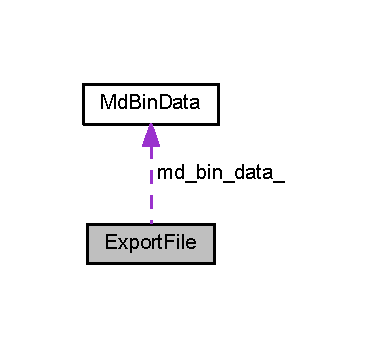
\includegraphics[width=177pt]{class_export_file__coll__graph}
\end{center}
\end{figure}
\subsection*{公開メンバ関数}
\begin{DoxyCompactItemize}
\item 
void \mbox{\hyperlink{class_export_file_a8b1ef14ae42180a8bf491d4d7a4ceb63}{set\+Md\+Bin\+Data}} (\mbox{\hyperlink{class_md_bin_data}{Md\+Bin\+Data}} $\ast$md\+\_\+bin\+\_\+data)
\begin{DoxyCompactList}\small\item\em Md\+Binデータ設定関数 \end{DoxyCompactList}\item 
void \mbox{\hyperlink{class_export_file_a9dd6b27de162bee08b51eb2ae62d8e17}{set\+Axis}} (Fbx\+Axis\+System axis)
\begin{DoxyCompactList}\small\item\em 軸設定関数 \end{DoxyCompactList}\item 
void \mbox{\hyperlink{class_export_file_aadb97e06e12bbe978e5527b4b540ece8}{Export}} (std\+::string $\ast$file\+\_\+path)
\begin{DoxyCompactList}\small\item\em 出力関数 \end{DoxyCompactList}\end{DoxyCompactItemize}
\subsection*{非公開メンバ関数}
\begin{DoxyCompactItemize}
\item 
bool \mbox{\hyperlink{class_export_file_a16e769db1683d63e0e4dbf809bd8704e}{Export\+Of\+Md\+Bin\+File}} ()
\begin{DoxyCompactList}\small\item\em Md\+Binファイルの出力関数 \end{DoxyCompactList}\item 
void \mbox{\hyperlink{class_export_file_ab8a6f3c0bf115e400beb188bc95b3d5c}{Export\+Of\+Log\+File}} ()
\begin{DoxyCompactList}\small\item\em ログファイルの出力関数 \end{DoxyCompactList}\item 
void \mbox{\hyperlink{class_export_file_a1a5927dcc9f77a33c3cde8e0f15161f3}{Export\+Of\+Material\+Log\+File}} (std\+::string $\ast$directory\+\_\+path)
\begin{DoxyCompactList}\small\item\em マテリアルログファイルの出力関数 \end{DoxyCompactList}\item 
void \mbox{\hyperlink{class_export_file_a4469089d40e6b28e1468f100cb2edb9d}{Export\+Of\+Mesh\+Log\+File}} (std\+::string $\ast$directory\+\_\+path)
\begin{DoxyCompactList}\small\item\em メッシュログファイルの出力関数 \end{DoxyCompactList}\item 
void \mbox{\hyperlink{class_export_file_a183be4cce0cdd02ac41f5d02dc4499ee}{Create\+File\+Name}} (std\+::string $\ast$file\+\_\+path)
\begin{DoxyCompactList}\small\item\em ファイル名作成関数 \end{DoxyCompactList}\item 
void \mbox{\hyperlink{class_export_file_af2c0b760712fc2806e030e4d30fc9599}{Create\+Export\+Directory\+Path}} ()
\begin{DoxyCompactList}\small\item\em 出力ディレクトリ名作成関数 \end{DoxyCompactList}\item 
void \mbox{\hyperlink{class_export_file_aab917dac60913d7aa73d458a82c4e29d}{Create\+Log\+Directory\+Path}} (std\+::string $\ast$material\+\_\+directory\+\_\+path, std\+::string $\ast$mesh\+\_\+directory\+\_\+path)
\begin{DoxyCompactList}\small\item\em ログディレクトリ名作成関数 \end{DoxyCompactList}\item 
void \mbox{\hyperlink{class_export_file_abf4344f171c496296579d9ad6d974afe}{Create\+Index\+Directory\+Path}} (std\+::string $\ast$index\+\_\+directory\+\_\+path, std\+::string $\ast$directory\+\_\+path, int index)
\begin{DoxyCompactList}\small\item\em インデックスディレクトリ名作成関数 \end{DoxyCompactList}\item 
void \mbox{\hyperlink{class_export_file_ad171b58b3ee1f84ed22a60afe55f4096}{Create\+Export\+Directory}} (std\+::string $\ast$directory\+\_\+path)
\begin{DoxyCompactList}\small\item\em 出力ディレクトリの作成関数 \end{DoxyCompactList}\item 
void \mbox{\hyperlink{class_export_file_a28a889812b0d24741f0466ff21ea4f82}{Create\+Export\+File\+Name}} (std\+::string $\ast$file\+\_\+name)
\begin{DoxyCompactList}\small\item\em 出力ファイル名作成関数 \end{DoxyCompactList}\item 
void \mbox{\hyperlink{class_export_file_a7c23d58ec17d273f55da9110745ef66b}{Create\+Index\+Log\+File\+Name}} (std\+::string $\ast$file\+\_\+name, int index)
\begin{DoxyCompactList}\small\item\em インデックスログファイル名作成関数 \end{DoxyCompactList}\item 
void \mbox{\hyperlink{class_export_file_afff4247767f7ad05091d60cba9279816}{Create\+Export\+Path}} (std\+::string $\ast$export\+\_\+file\+\_\+path, std\+::string $\ast$directory\+\_\+path, std\+::string $\ast$export\+\_\+file\+\_\+name)
\begin{DoxyCompactList}\small\item\em 出力パス作成関数 \end{DoxyCompactList}\end{DoxyCompactItemize}
\subsection*{非公開変数類}
\begin{DoxyCompactItemize}
\item 
\mbox{\hyperlink{class_md_bin_data}{Md\+Bin\+Data}} $\ast$ \mbox{\hyperlink{class_export_file_a21c28c8b20e7c7592c9b31e4f316e446}{md\+\_\+bin\+\_\+data\+\_\+}}
\begin{DoxyCompactList}\small\item\em Md\+Binデータ \end{DoxyCompactList}\item 
Fbx\+Axis\+System \mbox{\hyperlink{class_export_file_aa07d09fbe2283f5b69a3d001ce6bcc4c}{axis\+\_\+}}
\begin{DoxyCompactList}\small\item\em 軸 \end{DoxyCompactList}\item 
std\+::string \mbox{\hyperlink{class_export_file_a7b71765d0ac88a9e284a79e8fbbe4d4e}{file\+\_\+name\+\_\+}}
\begin{DoxyCompactList}\small\item\em 出力ディレクトリパス \end{DoxyCompactList}\item 
std\+::string \mbox{\hyperlink{class_export_file_ad61be755d6178b9f7f452f0e45343e02}{export\+\_\+directory\+\_\+path\+\_\+}}
\begin{DoxyCompactList}\small\item\em 出力ディレクトリパス \end{DoxyCompactList}\end{DoxyCompactItemize}


\subsection{詳解}
ファイル出力\+Class 

ファイル出力用\+Class 

 Export\+File.\+h の 27 行目に定義があります。



\subsection{関数詳解}
\mbox{\Hypertarget{class_export_file_ad171b58b3ee1f84ed22a60afe55f4096}\label{class_export_file_ad171b58b3ee1f84ed22a60afe55f4096}} 
\index{Export\+File@{Export\+File}!Create\+Export\+Directory@{Create\+Export\+Directory}}
\index{Create\+Export\+Directory@{Create\+Export\+Directory}!Export\+File@{Export\+File}}
\subsubsection{\texorpdfstring{Create\+Export\+Directory()}{CreateExportDirectory()}}
{\footnotesize\ttfamily void Export\+File\+::\+Create\+Export\+Directory (\begin{DoxyParamCaption}\item[{std\+::string $\ast$}]{directory\+\_\+path }\end{DoxyParamCaption})\hspace{0.3cm}{\ttfamily [private]}}



出力ディレクトリの作成関数 


\begin{DoxyParams}{引数}
{\em $\ast$directory\+\_\+path} & ディレクトリパス \\
\hline
\end{DoxyParams}

\begin{DoxyRetVals}{戻り値}
{\em void} & なし \\
\hline
\end{DoxyRetVals}


 Export\+File.\+cpp の 450 行目に定義があります。

\mbox{\Hypertarget{class_export_file_af2c0b760712fc2806e030e4d30fc9599}\label{class_export_file_af2c0b760712fc2806e030e4d30fc9599}} 
\index{Export\+File@{Export\+File}!Create\+Export\+Directory\+Path@{Create\+Export\+Directory\+Path}}
\index{Create\+Export\+Directory\+Path@{Create\+Export\+Directory\+Path}!Export\+File@{Export\+File}}
\subsubsection{\texorpdfstring{Create\+Export\+Directory\+Path()}{CreateExportDirectoryPath()}}
{\footnotesize\ttfamily void Export\+File\+::\+Create\+Export\+Directory\+Path (\begin{DoxyParamCaption}{ }\end{DoxyParamCaption})\hspace{0.3cm}{\ttfamily [private]}}



出力ディレクトリ名作成関数 


\begin{DoxyParams}{引数}
{\em void} & なし \\
\hline
\end{DoxyParams}

\begin{DoxyRetVals}{戻り値}
{\em void} & なし \\
\hline
\end{DoxyRetVals}


 Export\+File.\+cpp の 423 行目に定義があります。

\mbox{\Hypertarget{class_export_file_a28a889812b0d24741f0466ff21ea4f82}\label{class_export_file_a28a889812b0d24741f0466ff21ea4f82}} 
\index{Export\+File@{Export\+File}!Create\+Export\+File\+Name@{Create\+Export\+File\+Name}}
\index{Create\+Export\+File\+Name@{Create\+Export\+File\+Name}!Export\+File@{Export\+File}}
\subsubsection{\texorpdfstring{Create\+Export\+File\+Name()}{CreateExportFileName()}}
{\footnotesize\ttfamily void Export\+File\+::\+Create\+Export\+File\+Name (\begin{DoxyParamCaption}\item[{std\+::string $\ast$}]{file\+\_\+name }\end{DoxyParamCaption})\hspace{0.3cm}{\ttfamily [private]}}



出力ファイル名作成関数 


\begin{DoxyParams}{引数}
{\em $\ast$file\+\_\+name} & ファイル名 \\
\hline
\end{DoxyParams}

\begin{DoxyRetVals}{戻り値}
{\em void} & なし \\
\hline
\end{DoxyRetVals}


 Export\+File.\+cpp の 459 行目に定義があります。

\mbox{\Hypertarget{class_export_file_afff4247767f7ad05091d60cba9279816}\label{class_export_file_afff4247767f7ad05091d60cba9279816}} 
\index{Export\+File@{Export\+File}!Create\+Export\+Path@{Create\+Export\+Path}}
\index{Create\+Export\+Path@{Create\+Export\+Path}!Export\+File@{Export\+File}}
\subsubsection{\texorpdfstring{Create\+Export\+Path()}{CreateExportPath()}}
{\footnotesize\ttfamily void Export\+File\+::\+Create\+Export\+Path (\begin{DoxyParamCaption}\item[{std\+::string $\ast$}]{export\+\_\+file\+\_\+path,  }\item[{std\+::string $\ast$}]{directory\+\_\+path,  }\item[{std\+::string $\ast$}]{export\+\_\+file\+\_\+name }\end{DoxyParamCaption})\hspace{0.3cm}{\ttfamily [private]}}



出力パス作成関数 


\begin{DoxyParams}{引数}
{\em $\ast$export\+\_\+file\+\_\+path} & 出力パス \\
\hline
{\em $\ast$directory\+\_\+path} & ディレクトリパス \\
\hline
{\em $\ast$export\+\_\+file\+\_\+name} & 出力ファイル名 \\
\hline
\end{DoxyParams}

\begin{DoxyRetVals}{戻り値}
{\em void} & なし \\
\hline
\end{DoxyRetVals}


 Export\+File.\+cpp の 475 行目に定義があります。

\mbox{\Hypertarget{class_export_file_a183be4cce0cdd02ac41f5d02dc4499ee}\label{class_export_file_a183be4cce0cdd02ac41f5d02dc4499ee}} 
\index{Export\+File@{Export\+File}!Create\+File\+Name@{Create\+File\+Name}}
\index{Create\+File\+Name@{Create\+File\+Name}!Export\+File@{Export\+File}}
\subsubsection{\texorpdfstring{Create\+File\+Name()}{CreateFileName()}}
{\footnotesize\ttfamily void Export\+File\+::\+Create\+File\+Name (\begin{DoxyParamCaption}\item[{std\+::string $\ast$}]{file\+\_\+path }\end{DoxyParamCaption})\hspace{0.3cm}{\ttfamily [private]}}



ファイル名作成関数 


\begin{DoxyParams}{引数}
{\em $\ast$file\+\_\+path} & ファイルパス \\
\hline
\end{DoxyParams}

\begin{DoxyRetVals}{戻り値}
{\em void} & なし \\
\hline
\end{DoxyRetVals}


 Export\+File.\+cpp の 389 行目に定義があります。

\mbox{\Hypertarget{class_export_file_abf4344f171c496296579d9ad6d974afe}\label{class_export_file_abf4344f171c496296579d9ad6d974afe}} 
\index{Export\+File@{Export\+File}!Create\+Index\+Directory\+Path@{Create\+Index\+Directory\+Path}}
\index{Create\+Index\+Directory\+Path@{Create\+Index\+Directory\+Path}!Export\+File@{Export\+File}}
\subsubsection{\texorpdfstring{Create\+Index\+Directory\+Path()}{CreateIndexDirectoryPath()}}
{\footnotesize\ttfamily void Export\+File\+::\+Create\+Index\+Directory\+Path (\begin{DoxyParamCaption}\item[{std\+::string $\ast$}]{index\+\_\+directory\+\_\+path,  }\item[{std\+::string $\ast$}]{directory\+\_\+path,  }\item[{int}]{index }\end{DoxyParamCaption})\hspace{0.3cm}{\ttfamily [private]}}



インデックスディレクトリ名作成関数 


\begin{DoxyParams}{引数}
{\em $\ast$index\+\_\+directory\+\_\+path} & インデックスディレクトリパス \\
\hline
{\em $\ast$directory\+\_\+path} & ディレクトリパス \\
\hline
{\em index} & インデックス \\
\hline
\end{DoxyParams}

\begin{DoxyRetVals}{戻り値}
{\em void} & なし \\
\hline
\end{DoxyRetVals}


 Export\+File.\+cpp の 441 行目に定義があります。

\mbox{\Hypertarget{class_export_file_a7c23d58ec17d273f55da9110745ef66b}\label{class_export_file_a7c23d58ec17d273f55da9110745ef66b}} 
\index{Export\+File@{Export\+File}!Create\+Index\+Log\+File\+Name@{Create\+Index\+Log\+File\+Name}}
\index{Create\+Index\+Log\+File\+Name@{Create\+Index\+Log\+File\+Name}!Export\+File@{Export\+File}}
\subsubsection{\texorpdfstring{Create\+Index\+Log\+File\+Name()}{CreateIndexLogFileName()}}
{\footnotesize\ttfamily void Export\+File\+::\+Create\+Index\+Log\+File\+Name (\begin{DoxyParamCaption}\item[{std\+::string $\ast$}]{file\+\_\+name,  }\item[{int}]{index }\end{DoxyParamCaption})\hspace{0.3cm}{\ttfamily [private]}}



インデックスログファイル名作成関数 


\begin{DoxyParams}{引数}
{\em $\ast$file\+\_\+name} & ファイル名 \\
\hline
{\em index} & インデックス \\
\hline
\end{DoxyParams}

\begin{DoxyRetVals}{戻り値}
{\em void} & なし \\
\hline
\end{DoxyRetVals}


 Export\+File.\+cpp の 467 行目に定義があります。

\mbox{\Hypertarget{class_export_file_aab917dac60913d7aa73d458a82c4e29d}\label{class_export_file_aab917dac60913d7aa73d458a82c4e29d}} 
\index{Export\+File@{Export\+File}!Create\+Log\+Directory\+Path@{Create\+Log\+Directory\+Path}}
\index{Create\+Log\+Directory\+Path@{Create\+Log\+Directory\+Path}!Export\+File@{Export\+File}}
\subsubsection{\texorpdfstring{Create\+Log\+Directory\+Path()}{CreateLogDirectoryPath()}}
{\footnotesize\ttfamily void Export\+File\+::\+Create\+Log\+Directory\+Path (\begin{DoxyParamCaption}\item[{std\+::string $\ast$}]{material\+\_\+directory\+\_\+path,  }\item[{std\+::string $\ast$}]{mesh\+\_\+directory\+\_\+path }\end{DoxyParamCaption})\hspace{0.3cm}{\ttfamily [private]}}



ログディレクトリ名作成関数 


\begin{DoxyParams}{引数}
{\em $\ast$material\+\_\+directory\+\_\+path} & マテリアルディレクトリパス \\
\hline
{\em $\ast$mesh\+\_\+directory\+\_\+path} & メッシュディレクトリパス \\
\hline
\end{DoxyParams}

\begin{DoxyRetVals}{戻り値}
{\em void} & なし \\
\hline
\end{DoxyRetVals}


 Export\+File.\+cpp の 432 行目に定義があります。

\mbox{\Hypertarget{class_export_file_aadb97e06e12bbe978e5527b4b540ece8}\label{class_export_file_aadb97e06e12bbe978e5527b4b540ece8}} 
\index{Export\+File@{Export\+File}!Export@{Export}}
\index{Export@{Export}!Export\+File@{Export\+File}}
\subsubsection{\texorpdfstring{Export()}{Export()}}
{\footnotesize\ttfamily void Export\+File\+::\+Export (\begin{DoxyParamCaption}\item[{std\+::string $\ast$}]{file\+\_\+path }\end{DoxyParamCaption})}



出力関数 


\begin{DoxyParams}{引数}
{\em $\ast$file\+\_\+path} & ファイルパス \\
\hline
\end{DoxyParams}

\begin{DoxyRetVals}{戻り値}
{\em void} & なし \\
\hline
\end{DoxyRetVals}


 Export\+File.\+cpp の 44 行目に定義があります。

\mbox{\Hypertarget{class_export_file_ab8a6f3c0bf115e400beb188bc95b3d5c}\label{class_export_file_ab8a6f3c0bf115e400beb188bc95b3d5c}} 
\index{Export\+File@{Export\+File}!Export\+Of\+Log\+File@{Export\+Of\+Log\+File}}
\index{Export\+Of\+Log\+File@{Export\+Of\+Log\+File}!Export\+File@{Export\+File}}
\subsubsection{\texorpdfstring{Export\+Of\+Log\+File()}{ExportOfLogFile()}}
{\footnotesize\ttfamily void Export\+File\+::\+Export\+Of\+Log\+File (\begin{DoxyParamCaption}{ }\end{DoxyParamCaption})\hspace{0.3cm}{\ttfamily [private]}}



ログファイルの出力関数 


\begin{DoxyParams}{引数}
{\em void} & なし \\
\hline
\end{DoxyParams}

\begin{DoxyRetVals}{戻り値}
{\em void} & なし \\
\hline
\end{DoxyRetVals}


 Export\+File.\+cpp の 101 行目に定義があります。

\mbox{\Hypertarget{class_export_file_a1a5927dcc9f77a33c3cde8e0f15161f3}\label{class_export_file_a1a5927dcc9f77a33c3cde8e0f15161f3}} 
\index{Export\+File@{Export\+File}!Export\+Of\+Material\+Log\+File@{Export\+Of\+Material\+Log\+File}}
\index{Export\+Of\+Material\+Log\+File@{Export\+Of\+Material\+Log\+File}!Export\+File@{Export\+File}}
\subsubsection{\texorpdfstring{Export\+Of\+Material\+Log\+File()}{ExportOfMaterialLogFile()}}
{\footnotesize\ttfamily void Export\+File\+::\+Export\+Of\+Material\+Log\+File (\begin{DoxyParamCaption}\item[{std\+::string $\ast$}]{directory\+\_\+path }\end{DoxyParamCaption})\hspace{0.3cm}{\ttfamily [private]}}



マテリアルログファイルの出力関数 


\begin{DoxyParams}{引数}
{\em $\ast$directory\+\_\+path} & ディレクトリパス \\
\hline
\end{DoxyParams}

\begin{DoxyRetVals}{戻り値}
{\em void} & なし \\
\hline
\end{DoxyRetVals}


 Export\+File.\+cpp の 119 行目に定義があります。

\mbox{\Hypertarget{class_export_file_a16e769db1683d63e0e4dbf809bd8704e}\label{class_export_file_a16e769db1683d63e0e4dbf809bd8704e}} 
\index{Export\+File@{Export\+File}!Export\+Of\+Md\+Bin\+File@{Export\+Of\+Md\+Bin\+File}}
\index{Export\+Of\+Md\+Bin\+File@{Export\+Of\+Md\+Bin\+File}!Export\+File@{Export\+File}}
\subsubsection{\texorpdfstring{Export\+Of\+Md\+Bin\+File()}{ExportOfMdBinFile()}}
{\footnotesize\ttfamily bool Export\+File\+::\+Export\+Of\+Md\+Bin\+File (\begin{DoxyParamCaption}{ }\end{DoxyParamCaption})\hspace{0.3cm}{\ttfamily [private]}}



Md\+Binファイルの出力関数 


\begin{DoxyParams}{引数}
{\em void} & なし \\
\hline
\end{DoxyParams}

\begin{DoxyRetVals}{戻り値}
{\em bool} & 上書きの有無 \\
\hline
\end{DoxyRetVals}


 Export\+File.\+cpp の 63 行目に定義があります。

\mbox{\Hypertarget{class_export_file_a4469089d40e6b28e1468f100cb2edb9d}\label{class_export_file_a4469089d40e6b28e1468f100cb2edb9d}} 
\index{Export\+File@{Export\+File}!Export\+Of\+Mesh\+Log\+File@{Export\+Of\+Mesh\+Log\+File}}
\index{Export\+Of\+Mesh\+Log\+File@{Export\+Of\+Mesh\+Log\+File}!Export\+File@{Export\+File}}
\subsubsection{\texorpdfstring{Export\+Of\+Mesh\+Log\+File()}{ExportOfMeshLogFile()}}
{\footnotesize\ttfamily void Export\+File\+::\+Export\+Of\+Mesh\+Log\+File (\begin{DoxyParamCaption}\item[{std\+::string $\ast$}]{directory\+\_\+path }\end{DoxyParamCaption})\hspace{0.3cm}{\ttfamily [private]}}



メッシュログファイルの出力関数 


\begin{DoxyParams}{引数}
{\em $\ast$directory\+\_\+path} & ディレクトリパス \\
\hline
\end{DoxyParams}

\begin{DoxyRetVals}{戻り値}
{\em void} & なし \\
\hline
\end{DoxyRetVals}


 Export\+File.\+cpp の 186 行目に定義があります。

\mbox{\Hypertarget{class_export_file_a9dd6b27de162bee08b51eb2ae62d8e17}\label{class_export_file_a9dd6b27de162bee08b51eb2ae62d8e17}} 
\index{Export\+File@{Export\+File}!set\+Axis@{set\+Axis}}
\index{set\+Axis@{set\+Axis}!Export\+File@{Export\+File}}
\subsubsection{\texorpdfstring{set\+Axis()}{setAxis()}}
{\footnotesize\ttfamily void Export\+File\+::set\+Axis (\begin{DoxyParamCaption}\item[{Fbx\+Axis\+System}]{axis }\end{DoxyParamCaption})}



軸設定関数 


\begin{DoxyParams}{引数}
{\em axis} & 軸 \\
\hline
\end{DoxyParams}

\begin{DoxyRetVals}{戻り値}
{\em void} & なし \\
\hline
\end{DoxyRetVals}


 Export\+File.\+cpp の 34 行目に定義があります。

\mbox{\Hypertarget{class_export_file_a8b1ef14ae42180a8bf491d4d7a4ceb63}\label{class_export_file_a8b1ef14ae42180a8bf491d4d7a4ceb63}} 
\index{Export\+File@{Export\+File}!set\+Md\+Bin\+Data@{set\+Md\+Bin\+Data}}
\index{set\+Md\+Bin\+Data@{set\+Md\+Bin\+Data}!Export\+File@{Export\+File}}
\subsubsection{\texorpdfstring{set\+Md\+Bin\+Data()}{setMdBinData()}}
{\footnotesize\ttfamily void Export\+File\+::set\+Md\+Bin\+Data (\begin{DoxyParamCaption}\item[{\mbox{\hyperlink{class_md_bin_data}{Md\+Bin\+Data}} $\ast$}]{md\+\_\+bin\+\_\+data }\end{DoxyParamCaption})}



Md\+Binデータ設定関数 


\begin{DoxyParams}{引数}
{\em $\ast$md\+\_\+bin\+\_\+data} & Md\+Binデータ \\
\hline
\end{DoxyParams}

\begin{DoxyRetVals}{戻り値}
{\em void} & なし \\
\hline
\end{DoxyRetVals}


 Export\+File.\+cpp の 27 行目に定義があります。



\subsection{メンバ詳解}
\mbox{\Hypertarget{class_export_file_aa07d09fbe2283f5b69a3d001ce6bcc4c}\label{class_export_file_aa07d09fbe2283f5b69a3d001ce6bcc4c}} 
\index{Export\+File@{Export\+File}!axis\+\_\+@{axis\+\_\+}}
\index{axis\+\_\+@{axis\+\_\+}!Export\+File@{Export\+File}}
\subsubsection{\texorpdfstring{axis\+\_\+}{axis\_}}
{\footnotesize\ttfamily Fbx\+Axis\+System Export\+File\+::axis\+\_\+\hspace{0.3cm}{\ttfamily [private]}}



軸 



 Export\+File.\+h の 34 行目に定義があります。

\mbox{\Hypertarget{class_export_file_ad61be755d6178b9f7f452f0e45343e02}\label{class_export_file_ad61be755d6178b9f7f452f0e45343e02}} 
\index{Export\+File@{Export\+File}!export\+\_\+directory\+\_\+path\+\_\+@{export\+\_\+directory\+\_\+path\+\_\+}}
\index{export\+\_\+directory\+\_\+path\+\_\+@{export\+\_\+directory\+\_\+path\+\_\+}!Export\+File@{Export\+File}}
\subsubsection{\texorpdfstring{export\+\_\+directory\+\_\+path\+\_\+}{export\_directory\_path\_}}
{\footnotesize\ttfamily std\+::string Export\+File\+::export\+\_\+directory\+\_\+path\+\_\+\hspace{0.3cm}{\ttfamily [private]}}



出力ディレクトリパス 



 Export\+File.\+h の 36 行目に定義があります。

\mbox{\Hypertarget{class_export_file_a7b71765d0ac88a9e284a79e8fbbe4d4e}\label{class_export_file_a7b71765d0ac88a9e284a79e8fbbe4d4e}} 
\index{Export\+File@{Export\+File}!file\+\_\+name\+\_\+@{file\+\_\+name\+\_\+}}
\index{file\+\_\+name\+\_\+@{file\+\_\+name\+\_\+}!Export\+File@{Export\+File}}
\subsubsection{\texorpdfstring{file\+\_\+name\+\_\+}{file\_name\_}}
{\footnotesize\ttfamily std\+::string Export\+File\+::file\+\_\+name\+\_\+\hspace{0.3cm}{\ttfamily [private]}}



出力ディレクトリパス 



 Export\+File.\+h の 35 行目に定義があります。

\mbox{\Hypertarget{class_export_file_a21c28c8b20e7c7592c9b31e4f316e446}\label{class_export_file_a21c28c8b20e7c7592c9b31e4f316e446}} 
\index{Export\+File@{Export\+File}!md\+\_\+bin\+\_\+data\+\_\+@{md\+\_\+bin\+\_\+data\+\_\+}}
\index{md\+\_\+bin\+\_\+data\+\_\+@{md\+\_\+bin\+\_\+data\+\_\+}!Export\+File@{Export\+File}}
\subsubsection{\texorpdfstring{md\+\_\+bin\+\_\+data\+\_\+}{md\_bin\_data\_}}
{\footnotesize\ttfamily \mbox{\hyperlink{class_md_bin_data}{Md\+Bin\+Data}}$\ast$ Export\+File\+::md\+\_\+bin\+\_\+data\+\_\+\hspace{0.3cm}{\ttfamily [private]}}



Md\+Binデータ 



 Export\+File.\+h の 33 行目に定義があります。



このクラス詳解は次のファイルから抽出されました\+:\begin{DoxyCompactItemize}
\item 
C\+:/\+H\+A\+L/\+P\+G関係/03\+\_\+作成プログラム/03\+\_\+\+H\+A\+L授業/就職作品/\+Fbx\+Converter/source/\+Export\+File/\mbox{\hyperlink{_export_file_8h}{Export\+File.\+h}}\item 
C\+:/\+H\+A\+L/\+P\+G関係/03\+\_\+作成プログラム/03\+\_\+\+H\+A\+L授業/就職作品/\+Fbx\+Converter/source/\+Export\+File/\mbox{\hyperlink{_export_file_8cpp}{Export\+File.\+cpp}}\end{DoxyCompactItemize}

\hypertarget{class_fbx_converter}{}\section{Fbx\+Converter クラス}
\label{class_fbx_converter}\index{Fbx\+Converter@{Fbx\+Converter}}


F\+B\+X変換器\+Class  




{\ttfamily \#include $<$Fbx\+Converter.\+h$>$}



Fbx\+Converter 連携図\nopagebreak
\begin{figure}[H]
\begin{center}
\leavevmode
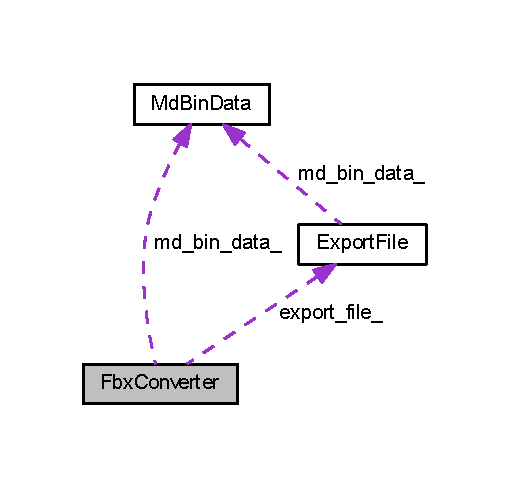
\includegraphics[width=245pt]{class_fbx_converter__coll__graph}
\end{center}
\end{figure}
\subsection*{公開メンバ関数}
\begin{DoxyCompactItemize}
\item 
bool \mbox{\hyperlink{class_fbx_converter_ad42745849ed5fbd2a6b332004a21a667}{Init}} ()
\begin{DoxyCompactList}\small\item\em 初期化関数 \end{DoxyCompactList}\item 
void \mbox{\hyperlink{class_fbx_converter_ab41f9b165cb34a294bb2c5da778f542b}{Uninit}} ()
\begin{DoxyCompactList}\small\item\em 終了関数 \end{DoxyCompactList}\item 
bool \mbox{\hyperlink{class_fbx_converter_aecd6ebf6aec9616bd609f6ebfc3a557e}{Convert\+To\+Md\+Bin}} (std\+::string $\ast$file\+\_\+path)
\begin{DoxyCompactList}\small\item\em Md\+Binへ変換関数 \end{DoxyCompactList}\end{DoxyCompactItemize}
\subsection*{非公開メンバ関数}
\begin{DoxyCompactItemize}
\item 
bool \mbox{\hyperlink{class_fbx_converter_a5259c5ec8f57b412455d75ccebb27524}{Load}} (std\+::string $\ast$file\+\_\+path)
\begin{DoxyCompactList}\small\item\em 読み込み関数 \end{DoxyCompactList}\item 
void \mbox{\hyperlink{class_fbx_converter_a0f6070933510e57b4a781d97d46f7406}{Extract\+Frame\+Data}} (Fbx\+Importer $\ast$importer)
\begin{DoxyCompactList}\small\item\em フレーム情報抽出関数 \end{DoxyCompactList}\item 
bool \mbox{\hyperlink{class_fbx_converter_ab0e56fde4c4e0f5bc846e7a6cd7f8a19}{Extract\+Data}} ()
\begin{DoxyCompactList}\small\item\em データ抽出関数 \end{DoxyCompactList}\item 
void \mbox{\hyperlink{class_fbx_converter_accf269065c211ffb8fc77634bf8dbee9}{Extract\+Material\+Data}} ()
\begin{DoxyCompactList}\small\item\em マテリアルデータの抽出関数 \end{DoxyCompactList}\item 
void \mbox{\hyperlink{class_fbx_converter_a4e1c69b9948c7aa9659a80ba3ba85f9f}{Extract\+Mesh\+Data}} ()
\begin{DoxyCompactList}\small\item\em メッシュデータの抽出関数 \end{DoxyCompactList}\item 
void \mbox{\hyperlink{class_fbx_converter_ae0180e652e003309edeb721f6d88e378}{Extract\+Material\+Name}} (int material\+\_\+index, Fbx\+Surface\+Material $\ast$material)
\begin{DoxyCompactList}\small\item\em マテリアル名の抽出関数 \end{DoxyCompactList}\item 
void \mbox{\hyperlink{class_fbx_converter_a95cb085115d7832311264e9d27b5fb72}{Extract\+Ambient\+Data}} (int material\+\_\+index, Fbx\+Surface\+Material $\ast$material)
\begin{DoxyCompactList}\small\item\em アンビエントデータの抽出関数 \end{DoxyCompactList}\item 
void \mbox{\hyperlink{class_fbx_converter_a60e517313041e75f081effceb74e7c56}{Extract\+Diffuse\+Data}} (int material\+\_\+index, Fbx\+Surface\+Material $\ast$material)
\begin{DoxyCompactList}\small\item\em ディフューズデータの抽出関数 \end{DoxyCompactList}\item 
void \mbox{\hyperlink{class_fbx_converter_ae43f5f7858379aa57f1dbc1373c66b77}{Extract\+Emissive\+Data}} (int material\+\_\+index, Fbx\+Surface\+Material $\ast$material)
\begin{DoxyCompactList}\small\item\em エミッシブデータの抽出関数 \end{DoxyCompactList}\item 
void \mbox{\hyperlink{class_fbx_converter_abc1470186342a7aabb60818cd4813a1a}{Extract\+Bump\+Data}} (int material\+\_\+index, Fbx\+Surface\+Material $\ast$material)
\begin{DoxyCompactList}\small\item\em バンプデータの抽出関数 \end{DoxyCompactList}\item 
void \mbox{\hyperlink{class_fbx_converter_a888c4e3d638aa79fa524b85a67f01f5d}{Extract\+Transparent\+Data}} (int material\+\_\+index, Fbx\+Surface\+Material $\ast$material)
\begin{DoxyCompactList}\small\item\em トランスペアレントデータの抽出関数 \end{DoxyCompactList}\item 
void \mbox{\hyperlink{class_fbx_converter_a2ff36051144ed83860d0287a953778b4}{Extract\+Specular\+Data}} (int material\+\_\+index, Fbx\+Surface\+Material $\ast$material)
\begin{DoxyCompactList}\small\item\em スペキュラデータの抽出関数 \end{DoxyCompactList}\item 
void \mbox{\hyperlink{class_fbx_converter_aa2d0d302ad6691934164dfdf1f5f6590}{Extract\+Power\+Data}} (int material\+\_\+index, Fbx\+Surface\+Material $\ast$material)
\begin{DoxyCompactList}\small\item\em パワー(シャイネス)データの抽出関数 \end{DoxyCompactList}\item 
void \mbox{\hyperlink{class_fbx_converter_a25d2148fb64c484684c7eb856e9ae255}{Extract\+Reflection\+Data}} (int material\+\_\+index, Fbx\+Surface\+Material $\ast$material)
\begin{DoxyCompactList}\small\item\em リフレクションデータの抽出関数 \end{DoxyCompactList}\item 
void \mbox{\hyperlink{class_fbx_converter_a59039fa4ffde0cbe8fa269e71878b0da}{Extract\+Texture\+Data}} (int material\+\_\+index, Fbx\+Property property, \mbox{\hyperlink{class_md_bin_data_1_1_material_1_1_texture_a30fadb7216d0650de284e2fd875868ae}{Md\+Bin\+Data\+::\+Material\+::\+Texture\+::\+Type}} texture\+\_\+type)
\begin{DoxyCompactList}\small\item\em テクスチャデータの抽出関数 \end{DoxyCompactList}\item 
void \mbox{\hyperlink{class_fbx_converter_ae7d26c94b5926ab4477f93926f6d345d}{Extract\+File\+Name}} (std\+::string $\ast$file\+\_\+name, std\+::string $\ast$file\+\_\+path)
\begin{DoxyCompactList}\small\item\em ファイル名抽出関数 \end{DoxyCompactList}\item 
void \mbox{\hyperlink{class_fbx_converter_a476feb886d898a64f88a0b23cf10651a}{Extract\+Index\+Data}} (int mesh\+\_\+index, Fbx\+Mesh $\ast$mesh)
\begin{DoxyCompactList}\small\item\em インデックスデータの抽出関数 \end{DoxyCompactList}\item 
void \mbox{\hyperlink{class_fbx_converter_adaa3676e36092b4a28a1748ac01dfa75}{Extract\+Vertex\+Data}} (int mesh\+\_\+index, Fbx\+Mesh $\ast$mesh)
\begin{DoxyCompactList}\small\item\em 頂点データの抽出関数 \end{DoxyCompactList}\item 
void \mbox{\hyperlink{class_fbx_converter_a1333d3fe7a3ab69f7121265117e56b7f}{Extract\+Normal\+Data}} (int mesh\+\_\+index, Fbx\+Mesh $\ast$mesh)
\begin{DoxyCompactList}\small\item\em 法線データの抽出関数 \end{DoxyCompactList}\item 
void \mbox{\hyperlink{class_fbx_converter_a06cbfb7a211fc212e74de160e809ef35}{Extract\+U\+V\+Set\+Data}} (int mesh\+\_\+index, Fbx\+Mesh $\ast$mesh)
\begin{DoxyCompactList}\small\item\em U\+Vセットデータの抽出関数 \end{DoxyCompactList}\item 
void \mbox{\hyperlink{class_fbx_converter_a3f07e7dae9ba8bcb83dca611aeb5b3a0}{Extract\+Animation\+Data}} (int mesh\+\_\+index, Fbx\+Mesh $\ast$mesh)
\begin{DoxyCompactList}\small\item\em アニメーションデータの抽出関数 \end{DoxyCompactList}\item 
void \mbox{\hyperlink{class_fbx_converter_a0df95f11a3cd66ba0ecf06244efe52e7}{Extract\+Bone\+Data}} (int mesh\+\_\+index, Fbx\+Cluster $\ast$cluster)
\begin{DoxyCompactList}\small\item\em ボーンデータの抽出関数 \end{DoxyCompactList}\item 
void \mbox{\hyperlink{class_fbx_converter_a744068ceddd573d1add39a484e25bdc6}{Extract\+Bone\+Weight\+Data}} (int mesh\+\_\+index, std\+::vector$<$ \mbox{\hyperlink{class_md_bin_data_1_1_mesh_1_1_bone_weight}{Md\+Bin\+Data\+::\+Mesh\+::\+Bone\+Weight}} $>$ $\ast$save\+\_\+bone\+\_\+weight\+\_\+array, Fbx\+Cluster $\ast$cluster)
\begin{DoxyCompactList}\small\item\em ボーンの重みデータの抽出関数 \end{DoxyCompactList}\item 
void \mbox{\hyperlink{class_fbx_converter_a4587ba56496d6aa8cdfdd9ea92300c46}{Change\+Matrix}} (\mbox{\hyperlink{class_md_bin_data_1_1_matrix}{Md\+Bin\+Data\+::\+Matrix}} $\ast$bone\+\_\+matrix, Fbx\+A\+Matrix $\ast$fbx\+\_\+matrix)
\begin{DoxyCompactList}\small\item\em 行列変換関数 \end{DoxyCompactList}\item 
void \mbox{\hyperlink{class_fbx_converter_aa5a81e3afe4ea2bdc101863f6c1f0326}{Associate\+With\+Material\+Data}} (int mesh\+\_\+index, Fbx\+Mesh $\ast$mesh)
\begin{DoxyCompactList}\small\item\em マテリアルデータとの関連付け関数 \end{DoxyCompactList}\item 
void \mbox{\hyperlink{class_fbx_converter_a0d669f32bb338dffeb5d1989a0b374d7}{Associating\+U\+V\+Set\+Data\+And\+Texture}} (int mesh\+\_\+index)
\begin{DoxyCompactList}\small\item\em U\+Vセットデータとテクスチャの関連付け関数 \end{DoxyCompactList}\item 
void \mbox{\hyperlink{class_fbx_converter_a471d98b3d59a3f32dd2403577deebad7}{Convert\+To\+Full\+Path\+Of\+U\+T\+F8}} (std\+::string $\ast$file\+\_\+path)
\begin{DoxyCompactList}\small\item\em U\+T\+F8のフルパスへ変換関数 \end{DoxyCompactList}\end{DoxyCompactItemize}
\subsection*{非公開変数類}
\begin{DoxyCompactItemize}
\item 
Fbx\+Manager $\ast$ \mbox{\hyperlink{class_fbx_converter_a5c236830d34901e79030647478d3ef1b}{manager\+\_\+}} = nullptr
\begin{DoxyCompactList}\small\item\em F\+B\+Xマネージャ \end{DoxyCompactList}\item 
Fbx\+Scene $\ast$ \mbox{\hyperlink{class_fbx_converter_a64600b8f5225b7147c72105558386d78}{scene\+\_\+}} = nullptr
\begin{DoxyCompactList}\small\item\em シーン \end{DoxyCompactList}\item 
Fbx\+Node $\ast$ \mbox{\hyperlink{class_fbx_converter_ad5a43f9ee7bcf730c5f95e0ec63a4b8e}{root\+\_\+node\+\_\+}} = nullptr
\begin{DoxyCompactList}\small\item\em ルートノード \end{DoxyCompactList}\item 
Fbx\+Axis\+System \mbox{\hyperlink{class_fbx_converter_a36b80ea020d572dfff02125724af4c53}{axis\+\_\+system\+\_\+}}
\begin{DoxyCompactList}\small\item\em 座標系の種類 \end{DoxyCompactList}\item 
bool \mbox{\hyperlink{class_fbx_converter_ad88043ffdcbe995d3f1f8649395e58c9}{is\+\_\+reverse\+\_\+alpha\+\_\+}} = false
\begin{DoxyCompactList}\small\item\em α値の反転フラグ \end{DoxyCompactList}\item 
std\+::string \mbox{\hyperlink{class_fbx_converter_a542178c31548a51cd28726e2154c0f70}{directory\+\_\+path\+\_\+}}
\begin{DoxyCompactList}\small\item\em ディレクトリパス \end{DoxyCompactList}\item 
Fbx\+Time \mbox{\hyperlink{class_fbx_converter_a6d72d42a71572369aa2fed2f8710e696}{period\+\_\+}}
\begin{DoxyCompactList}\small\item\em 1フレームの時間 \end{DoxyCompactList}\item 
int \mbox{\hyperlink{class_fbx_converter_a5ce2f08e1d77044d628949d3ad7572ca}{animation\+\_\+start\+\_\+frame\+\_\+num\+\_\+}} = 0
\begin{DoxyCompactList}\small\item\em アニメーション開始フレーム数 \end{DoxyCompactList}\item 
int \mbox{\hyperlink{class_fbx_converter_ad7d116416b9d843c79ca282841e398c7}{animation\+\_\+stop\+\_\+frame\+\_\+num\+\_\+}} = 0
\begin{DoxyCompactList}\small\item\em アニメーション停止フレーム数 \end{DoxyCompactList}\item 
int \mbox{\hyperlink{class_fbx_converter_adcb0b8e16e923953c16d1a171df50190}{all\+\_\+animation\+\_\+frame\+\_\+num\+\_\+}} = 0
\begin{DoxyCompactList}\small\item\em アニメーションフレーム数 \end{DoxyCompactList}\item 
\mbox{\hyperlink{class_md_bin_data}{Md\+Bin\+Data}} \mbox{\hyperlink{class_fbx_converter_a637b9f53af4fbc31a961e9e2204dfaf5}{md\+\_\+bin\+\_\+data\+\_\+}}
\begin{DoxyCompactList}\small\item\em Md\+Binデータ \end{DoxyCompactList}\item 
\mbox{\hyperlink{class_export_file}{Export\+File}} \mbox{\hyperlink{class_fbx_converter_ac840641172dc753b399902ea928b4ff6}{export\+\_\+file\+\_\+}}
\begin{DoxyCompactList}\small\item\em ファイル出力 \end{DoxyCompactList}\end{DoxyCompactItemize}


\subsection{詳解}
F\+B\+X変換器\+Class 

F\+B\+X変換器\+Class 

 Fbx\+Converter.\+h の 28 行目に定義があります。



\subsection{関数詳解}
\mbox{\Hypertarget{class_fbx_converter_aa5a81e3afe4ea2bdc101863f6c1f0326}\label{class_fbx_converter_aa5a81e3afe4ea2bdc101863f6c1f0326}} 
\index{Fbx\+Converter@{Fbx\+Converter}!Associate\+With\+Material\+Data@{Associate\+With\+Material\+Data}}
\index{Associate\+With\+Material\+Data@{Associate\+With\+Material\+Data}!Fbx\+Converter@{Fbx\+Converter}}
\subsubsection{\texorpdfstring{Associate\+With\+Material\+Data()}{AssociateWithMaterialData()}}
{\footnotesize\ttfamily void Fbx\+Converter\+::\+Associate\+With\+Material\+Data (\begin{DoxyParamCaption}\item[{int}]{mesh\+\_\+index,  }\item[{Fbx\+Mesh $\ast$}]{mesh }\end{DoxyParamCaption})\hspace{0.3cm}{\ttfamily [private]}}



マテリアルデータとの関連付け関数 


\begin{DoxyParams}{引数}
{\em $\ast$mesh\+\_\+index} & メッシュのインデックス \\
\hline
{\em $\ast$mesh} & メッシュ \\
\hline
\end{DoxyParams}

\begin{DoxyRetVals}{戻り値}
{\em void} & なし \\
\hline
\end{DoxyRetVals}


 Fbx\+Converter.\+cpp の 744 行目に定義があります。

\mbox{\Hypertarget{class_fbx_converter_a0d669f32bb338dffeb5d1989a0b374d7}\label{class_fbx_converter_a0d669f32bb338dffeb5d1989a0b374d7}} 
\index{Fbx\+Converter@{Fbx\+Converter}!Associating\+U\+V\+Set\+Data\+And\+Texture@{Associating\+U\+V\+Set\+Data\+And\+Texture}}
\index{Associating\+U\+V\+Set\+Data\+And\+Texture@{Associating\+U\+V\+Set\+Data\+And\+Texture}!Fbx\+Converter@{Fbx\+Converter}}
\subsubsection{\texorpdfstring{Associating\+U\+V\+Set\+Data\+And\+Texture()}{AssociatingUVSetDataAndTexture()}}
{\footnotesize\ttfamily void Fbx\+Converter\+::\+Associating\+U\+V\+Set\+Data\+And\+Texture (\begin{DoxyParamCaption}\item[{int}]{mesh\+\_\+index }\end{DoxyParamCaption})\hspace{0.3cm}{\ttfamily [private]}}



U\+Vセットデータとテクスチャの関連付け関数 


\begin{DoxyParams}{引数}
{\em $\ast$mesh\+\_\+index} & メッシュのインデックス \\
\hline
\end{DoxyParams}

\begin{DoxyRetVals}{戻り値}
{\em void} & なし \\
\hline
\end{DoxyRetVals}


 Fbx\+Converter.\+cpp の 786 行目に定義があります。

\mbox{\Hypertarget{class_fbx_converter_a4587ba56496d6aa8cdfdd9ea92300c46}\label{class_fbx_converter_a4587ba56496d6aa8cdfdd9ea92300c46}} 
\index{Fbx\+Converter@{Fbx\+Converter}!Change\+Matrix@{Change\+Matrix}}
\index{Change\+Matrix@{Change\+Matrix}!Fbx\+Converter@{Fbx\+Converter}}
\subsubsection{\texorpdfstring{Change\+Matrix()}{ChangeMatrix()}}
{\footnotesize\ttfamily void Fbx\+Converter\+::\+Change\+Matrix (\begin{DoxyParamCaption}\item[{\mbox{\hyperlink{class_md_bin_data_1_1_matrix}{Md\+Bin\+Data\+::\+Matrix}} $\ast$}]{bone\+\_\+matrix,  }\item[{Fbx\+A\+Matrix $\ast$}]{fbx\+\_\+matrix }\end{DoxyParamCaption})\hspace{0.3cm}{\ttfamily [private]}}



行列変換関数 


\begin{DoxyParams}{引数}
{\em $\ast$bone\+\_\+matrix} & ボーン行列 \\
\hline
{\em $\ast$fbx\+\_\+matrix} & F\+B\+X行列 \\
\hline
\end{DoxyParams}

\begin{DoxyRetVals}{戻り値}
{\em void} & なし \\
\hline
\end{DoxyRetVals}


 Fbx\+Converter.\+cpp の 730 行目に定義があります。

\mbox{\Hypertarget{class_fbx_converter_a471d98b3d59a3f32dd2403577deebad7}\label{class_fbx_converter_a471d98b3d59a3f32dd2403577deebad7}} 
\index{Fbx\+Converter@{Fbx\+Converter}!Convert\+To\+Full\+Path\+Of\+U\+T\+F8@{Convert\+To\+Full\+Path\+Of\+U\+T\+F8}}
\index{Convert\+To\+Full\+Path\+Of\+U\+T\+F8@{Convert\+To\+Full\+Path\+Of\+U\+T\+F8}!Fbx\+Converter@{Fbx\+Converter}}
\subsubsection{\texorpdfstring{Convert\+To\+Full\+Path\+Of\+U\+T\+F8()}{ConvertToFullPathOfUTF8()}}
{\footnotesize\ttfamily void Fbx\+Converter\+::\+Convert\+To\+Full\+Path\+Of\+U\+T\+F8 (\begin{DoxyParamCaption}\item[{std\+::string $\ast$}]{file\+\_\+path }\end{DoxyParamCaption})\hspace{0.3cm}{\ttfamily [private]}}



U\+T\+F8のフルパスへ変換関数 


\begin{DoxyParams}{引数}
{\em $\ast$file\+\_\+path} & ファイルパス \\
\hline
\end{DoxyParams}

\begin{DoxyRetVals}{戻り値}
{\em void} & なし \\
\hline
\end{DoxyRetVals}


 Fbx\+Converter.\+cpp の 808 行目に定義があります。

\mbox{\Hypertarget{class_fbx_converter_aecd6ebf6aec9616bd609f6ebfc3a557e}\label{class_fbx_converter_aecd6ebf6aec9616bd609f6ebfc3a557e}} 
\index{Fbx\+Converter@{Fbx\+Converter}!Convert\+To\+Md\+Bin@{Convert\+To\+Md\+Bin}}
\index{Convert\+To\+Md\+Bin@{Convert\+To\+Md\+Bin}!Fbx\+Converter@{Fbx\+Converter}}
\subsubsection{\texorpdfstring{Convert\+To\+Md\+Bin()}{ConvertToMdBin()}}
{\footnotesize\ttfamily bool Fbx\+Converter\+::\+Convert\+To\+Md\+Bin (\begin{DoxyParamCaption}\item[{std\+::string $\ast$}]{file\+\_\+path }\end{DoxyParamCaption})}



Md\+Binへ変換関数 


\begin{DoxyParams}{引数}
{\em $\ast$file\+\_\+path} & ファイルパス \\
\hline
\end{DoxyParams}

\begin{DoxyRetVals}{戻り値}
{\em bool} & 変換成功の有無 \\
\hline
\end{DoxyRetVals}


 Fbx\+Converter.\+cpp の 70 行目に定義があります。

\mbox{\Hypertarget{class_fbx_converter_a95cb085115d7832311264e9d27b5fb72}\label{class_fbx_converter_a95cb085115d7832311264e9d27b5fb72}} 
\index{Fbx\+Converter@{Fbx\+Converter}!Extract\+Ambient\+Data@{Extract\+Ambient\+Data}}
\index{Extract\+Ambient\+Data@{Extract\+Ambient\+Data}!Fbx\+Converter@{Fbx\+Converter}}
\subsubsection{\texorpdfstring{Extract\+Ambient\+Data()}{ExtractAmbientData()}}
{\footnotesize\ttfamily void Fbx\+Converter\+::\+Extract\+Ambient\+Data (\begin{DoxyParamCaption}\item[{int}]{material\+\_\+index,  }\item[{Fbx\+Surface\+Material $\ast$}]{material }\end{DoxyParamCaption})\hspace{0.3cm}{\ttfamily [private]}}



アンビエントデータの抽出関数 


\begin{DoxyParams}{引数}
{\em $\ast$material\+\_\+index} & マテリアルのインデックス \\
\hline
{\em $\ast$material} & マテリアル \\
\hline
\end{DoxyParams}

\begin{DoxyRetVals}{戻り値}
{\em void} & なし \\
\hline
\end{DoxyRetVals}


 Fbx\+Converter.\+cpp の 311 行目に定義があります。

\mbox{\Hypertarget{class_fbx_converter_a3f07e7dae9ba8bcb83dca611aeb5b3a0}\label{class_fbx_converter_a3f07e7dae9ba8bcb83dca611aeb5b3a0}} 
\index{Fbx\+Converter@{Fbx\+Converter}!Extract\+Animation\+Data@{Extract\+Animation\+Data}}
\index{Extract\+Animation\+Data@{Extract\+Animation\+Data}!Fbx\+Converter@{Fbx\+Converter}}
\subsubsection{\texorpdfstring{Extract\+Animation\+Data()}{ExtractAnimationData()}}
{\footnotesize\ttfamily void Fbx\+Converter\+::\+Extract\+Animation\+Data (\begin{DoxyParamCaption}\item[{int}]{mesh\+\_\+index,  }\item[{Fbx\+Mesh $\ast$}]{mesh }\end{DoxyParamCaption})\hspace{0.3cm}{\ttfamily [private]}}



アニメーションデータの抽出関数 


\begin{DoxyParams}{引数}
{\em $\ast$mesh\+\_\+index} & メッシュのインデックス \\
\hline
{\em $\ast$mesh} & メッシュ \\
\hline
\end{DoxyParams}

\begin{DoxyRetVals}{戻り値}
{\em void} & なし \\
\hline
\end{DoxyRetVals}


 Fbx\+Converter.\+cpp の 621 行目に定義があります。

\mbox{\Hypertarget{class_fbx_converter_a0df95f11a3cd66ba0ecf06244efe52e7}\label{class_fbx_converter_a0df95f11a3cd66ba0ecf06244efe52e7}} 
\index{Fbx\+Converter@{Fbx\+Converter}!Extract\+Bone\+Data@{Extract\+Bone\+Data}}
\index{Extract\+Bone\+Data@{Extract\+Bone\+Data}!Fbx\+Converter@{Fbx\+Converter}}
\subsubsection{\texorpdfstring{Extract\+Bone\+Data()}{ExtractBoneData()}}
{\footnotesize\ttfamily void Fbx\+Converter\+::\+Extract\+Bone\+Data (\begin{DoxyParamCaption}\item[{int}]{mesh\+\_\+index,  }\item[{Fbx\+Cluster $\ast$}]{cluster }\end{DoxyParamCaption})\hspace{0.3cm}{\ttfamily [private]}}



ボーンデータの抽出関数 


\begin{DoxyParams}{引数}
{\em $\ast$mesh\+\_\+index} & メッシュのインデックス \\
\hline
{\em $\ast$cluster} & クラスタ \\
\hline
\end{DoxyParams}

\begin{DoxyRetVals}{戻り値}
{\em void} & なし \\
\hline
\end{DoxyRetVals}


 Fbx\+Converter.\+cpp の 663 行目に定義があります。

\mbox{\Hypertarget{class_fbx_converter_a744068ceddd573d1add39a484e25bdc6}\label{class_fbx_converter_a744068ceddd573d1add39a484e25bdc6}} 
\index{Fbx\+Converter@{Fbx\+Converter}!Extract\+Bone\+Weight\+Data@{Extract\+Bone\+Weight\+Data}}
\index{Extract\+Bone\+Weight\+Data@{Extract\+Bone\+Weight\+Data}!Fbx\+Converter@{Fbx\+Converter}}
\subsubsection{\texorpdfstring{Extract\+Bone\+Weight\+Data()}{ExtractBoneWeightData()}}
{\footnotesize\ttfamily void Fbx\+Converter\+::\+Extract\+Bone\+Weight\+Data (\begin{DoxyParamCaption}\item[{int}]{mesh\+\_\+index,  }\item[{std\+::vector$<$ \mbox{\hyperlink{class_md_bin_data_1_1_mesh_1_1_bone_weight}{Md\+Bin\+Data\+::\+Mesh\+::\+Bone\+Weight}} $>$ $\ast$}]{save\+\_\+bone\+\_\+weight\+\_\+array,  }\item[{Fbx\+Cluster $\ast$}]{cluster }\end{DoxyParamCaption})\hspace{0.3cm}{\ttfamily [private]}}



ボーンの重みデータの抽出関数 


\begin{DoxyParams}{引数}
{\em $\ast$mesh\+\_\+index} & メッシュのインデックス \\
\hline
{\em $\ast$save\+\_\+bone\+\_\+weight\+\_\+array} & ボーンの重み保存用配列 \\
\hline
{\em $\ast$cluster} & クラスタ \\
\hline
\end{DoxyParams}

\begin{DoxyRetVals}{戻り値}
{\em void} & なし \\
\hline
\end{DoxyRetVals}


 Fbx\+Converter.\+cpp の 703 行目に定義があります。

\mbox{\Hypertarget{class_fbx_converter_abc1470186342a7aabb60818cd4813a1a}\label{class_fbx_converter_abc1470186342a7aabb60818cd4813a1a}} 
\index{Fbx\+Converter@{Fbx\+Converter}!Extract\+Bump\+Data@{Extract\+Bump\+Data}}
\index{Extract\+Bump\+Data@{Extract\+Bump\+Data}!Fbx\+Converter@{Fbx\+Converter}}
\subsubsection{\texorpdfstring{Extract\+Bump\+Data()}{ExtractBumpData()}}
{\footnotesize\ttfamily void Fbx\+Converter\+::\+Extract\+Bump\+Data (\begin{DoxyParamCaption}\item[{int}]{material\+\_\+index,  }\item[{Fbx\+Surface\+Material $\ast$}]{material }\end{DoxyParamCaption})\hspace{0.3cm}{\ttfamily [private]}}



バンプデータの抽出関数 


\begin{DoxyParams}{引数}
{\em $\ast$material\+\_\+index} & マテリアルのインデックス \\
\hline
{\em $\ast$material} & マテリアル \\
\hline
\end{DoxyParams}

\begin{DoxyRetVals}{戻り値}
{\em void} & なし \\
\hline
\end{DoxyRetVals}


 Fbx\+Converter.\+cpp の 380 行目に定義があります。

\mbox{\Hypertarget{class_fbx_converter_ab0e56fde4c4e0f5bc846e7a6cd7f8a19}\label{class_fbx_converter_ab0e56fde4c4e0f5bc846e7a6cd7f8a19}} 
\index{Fbx\+Converter@{Fbx\+Converter}!Extract\+Data@{Extract\+Data}}
\index{Extract\+Data@{Extract\+Data}!Fbx\+Converter@{Fbx\+Converter}}
\subsubsection{\texorpdfstring{Extract\+Data()}{ExtractData()}}
{\footnotesize\ttfamily bool Fbx\+Converter\+::\+Extract\+Data (\begin{DoxyParamCaption}{ }\end{DoxyParamCaption})\hspace{0.3cm}{\ttfamily [private]}}



データ抽出関数 


\begin{DoxyParams}{引数}
{\em void} & なし \\
\hline
\end{DoxyParams}

\begin{DoxyRetVals}{戻り値}
{\em bool} & データの抽出成功の有無 \\
\hline
\end{DoxyRetVals}


 Fbx\+Converter.\+cpp の 232 行目に定義があります。

\mbox{\Hypertarget{class_fbx_converter_a60e517313041e75f081effceb74e7c56}\label{class_fbx_converter_a60e517313041e75f081effceb74e7c56}} 
\index{Fbx\+Converter@{Fbx\+Converter}!Extract\+Diffuse\+Data@{Extract\+Diffuse\+Data}}
\index{Extract\+Diffuse\+Data@{Extract\+Diffuse\+Data}!Fbx\+Converter@{Fbx\+Converter}}
\subsubsection{\texorpdfstring{Extract\+Diffuse\+Data()}{ExtractDiffuseData()}}
{\footnotesize\ttfamily void Fbx\+Converter\+::\+Extract\+Diffuse\+Data (\begin{DoxyParamCaption}\item[{int}]{material\+\_\+index,  }\item[{Fbx\+Surface\+Material $\ast$}]{material }\end{DoxyParamCaption})\hspace{0.3cm}{\ttfamily [private]}}



ディフューズデータの抽出関数 


\begin{DoxyParams}{引数}
{\em $\ast$material\+\_\+index} & マテリアルのインデックス \\
\hline
{\em $\ast$material} & マテリアル \\
\hline
\end{DoxyParams}

\begin{DoxyRetVals}{戻り値}
{\em void} & なし \\
\hline
\end{DoxyRetVals}


 Fbx\+Converter.\+cpp の 334 行目に定義があります。

\mbox{\Hypertarget{class_fbx_converter_ae43f5f7858379aa57f1dbc1373c66b77}\label{class_fbx_converter_ae43f5f7858379aa57f1dbc1373c66b77}} 
\index{Fbx\+Converter@{Fbx\+Converter}!Extract\+Emissive\+Data@{Extract\+Emissive\+Data}}
\index{Extract\+Emissive\+Data@{Extract\+Emissive\+Data}!Fbx\+Converter@{Fbx\+Converter}}
\subsubsection{\texorpdfstring{Extract\+Emissive\+Data()}{ExtractEmissiveData()}}
{\footnotesize\ttfamily void Fbx\+Converter\+::\+Extract\+Emissive\+Data (\begin{DoxyParamCaption}\item[{int}]{material\+\_\+index,  }\item[{Fbx\+Surface\+Material $\ast$}]{material }\end{DoxyParamCaption})\hspace{0.3cm}{\ttfamily [private]}}



エミッシブデータの抽出関数 


\begin{DoxyParams}{引数}
{\em $\ast$material\+\_\+index} & マテリアルのインデックス \\
\hline
{\em $\ast$material} & マテリアル \\
\hline
\end{DoxyParams}

\begin{DoxyRetVals}{戻り値}
{\em void} & なし \\
\hline
\end{DoxyRetVals}


 Fbx\+Converter.\+cpp の 357 行目に定義があります。

\mbox{\Hypertarget{class_fbx_converter_ae7d26c94b5926ab4477f93926f6d345d}\label{class_fbx_converter_ae7d26c94b5926ab4477f93926f6d345d}} 
\index{Fbx\+Converter@{Fbx\+Converter}!Extract\+File\+Name@{Extract\+File\+Name}}
\index{Extract\+File\+Name@{Extract\+File\+Name}!Fbx\+Converter@{Fbx\+Converter}}
\subsubsection{\texorpdfstring{Extract\+File\+Name()}{ExtractFileName()}}
{\footnotesize\ttfamily void Fbx\+Converter\+::\+Extract\+File\+Name (\begin{DoxyParamCaption}\item[{std\+::string $\ast$}]{file\+\_\+name,  }\item[{std\+::string $\ast$}]{file\+\_\+path }\end{DoxyParamCaption})\hspace{0.3cm}{\ttfamily [private]}}



ファイル名抽出関数 


\begin{DoxyParams}{引数}
{\em $\ast$file\+\_\+name} & ファイル名 \\
\hline
{\em $\ast$file\+\_\+path} & ファイルパス \\
\hline
\end{DoxyParams}

\begin{DoxyRetVals}{戻り値}
{\em void} & なし \\
\hline
\end{DoxyRetVals}


 Fbx\+Converter.\+cpp の 504 行目に定義があります。

\mbox{\Hypertarget{class_fbx_converter_a0f6070933510e57b4a781d97d46f7406}\label{class_fbx_converter_a0f6070933510e57b4a781d97d46f7406}} 
\index{Fbx\+Converter@{Fbx\+Converter}!Extract\+Frame\+Data@{Extract\+Frame\+Data}}
\index{Extract\+Frame\+Data@{Extract\+Frame\+Data}!Fbx\+Converter@{Fbx\+Converter}}
\subsubsection{\texorpdfstring{Extract\+Frame\+Data()}{ExtractFrameData()}}
{\footnotesize\ttfamily void Fbx\+Converter\+::\+Extract\+Frame\+Data (\begin{DoxyParamCaption}\item[{Fbx\+Importer $\ast$}]{importer }\end{DoxyParamCaption})\hspace{0.3cm}{\ttfamily [private]}}



フレーム情報抽出関数 


\begin{DoxyParams}{引数}
{\em $\ast$importer} & インポーター \\
\hline
\end{DoxyParams}

\begin{DoxyRetVals}{戻り値}
{\em void} & なし \\
\hline
\end{DoxyRetVals}


 Fbx\+Converter.\+cpp の 194 行目に定義があります。

\mbox{\Hypertarget{class_fbx_converter_a476feb886d898a64f88a0b23cf10651a}\label{class_fbx_converter_a476feb886d898a64f88a0b23cf10651a}} 
\index{Fbx\+Converter@{Fbx\+Converter}!Extract\+Index\+Data@{Extract\+Index\+Data}}
\index{Extract\+Index\+Data@{Extract\+Index\+Data}!Fbx\+Converter@{Fbx\+Converter}}
\subsubsection{\texorpdfstring{Extract\+Index\+Data()}{ExtractIndexData()}}
{\footnotesize\ttfamily void Fbx\+Converter\+::\+Extract\+Index\+Data (\begin{DoxyParamCaption}\item[{int}]{mesh\+\_\+index,  }\item[{Fbx\+Mesh $\ast$}]{mesh }\end{DoxyParamCaption})\hspace{0.3cm}{\ttfamily [private]}}



インデックスデータの抽出関数 


\begin{DoxyParams}{引数}
{\em $\ast$mesh\+\_\+index} & メッシュのインデックス \\
\hline
{\em $\ast$mesh} & メッシュ \\
\hline
\end{DoxyParams}

\begin{DoxyRetVals}{戻り値}
{\em void} & なし \\
\hline
\end{DoxyRetVals}


 Fbx\+Converter.\+cpp の 531 行目に定義があります。

\mbox{\Hypertarget{class_fbx_converter_accf269065c211ffb8fc77634bf8dbee9}\label{class_fbx_converter_accf269065c211ffb8fc77634bf8dbee9}} 
\index{Fbx\+Converter@{Fbx\+Converter}!Extract\+Material\+Data@{Extract\+Material\+Data}}
\index{Extract\+Material\+Data@{Extract\+Material\+Data}!Fbx\+Converter@{Fbx\+Converter}}
\subsubsection{\texorpdfstring{Extract\+Material\+Data()}{ExtractMaterialData()}}
{\footnotesize\ttfamily void Fbx\+Converter\+::\+Extract\+Material\+Data (\begin{DoxyParamCaption}{ }\end{DoxyParamCaption})\hspace{0.3cm}{\ttfamily [private]}}



マテリアルデータの抽出関数 


\begin{DoxyParams}{引数}
{\em void} & なし \\
\hline
\end{DoxyParams}

\begin{DoxyRetVals}{戻り値}
{\em void} & なし \\
\hline
\end{DoxyRetVals}


 Fbx\+Converter.\+cpp の 248 行目に定義があります。

\mbox{\Hypertarget{class_fbx_converter_ae0180e652e003309edeb721f6d88e378}\label{class_fbx_converter_ae0180e652e003309edeb721f6d88e378}} 
\index{Fbx\+Converter@{Fbx\+Converter}!Extract\+Material\+Name@{Extract\+Material\+Name}}
\index{Extract\+Material\+Name@{Extract\+Material\+Name}!Fbx\+Converter@{Fbx\+Converter}}
\subsubsection{\texorpdfstring{Extract\+Material\+Name()}{ExtractMaterialName()}}
{\footnotesize\ttfamily void Fbx\+Converter\+::\+Extract\+Material\+Name (\begin{DoxyParamCaption}\item[{int}]{material\+\_\+index,  }\item[{Fbx\+Surface\+Material $\ast$}]{material }\end{DoxyParamCaption})\hspace{0.3cm}{\ttfamily [private]}}



マテリアル名の抽出関数 


\begin{DoxyParams}{引数}
{\em $\ast$material\+\_\+index} & マテリアルのインデックス \\
\hline
{\em $\ast$material} & マテリアル \\
\hline
\end{DoxyParams}

\begin{DoxyRetVals}{戻り値}
{\em void} & なし \\
\hline
\end{DoxyRetVals}


 Fbx\+Converter.\+cpp の 304 行目に定義があります。

\mbox{\Hypertarget{class_fbx_converter_a4e1c69b9948c7aa9659a80ba3ba85f9f}\label{class_fbx_converter_a4e1c69b9948c7aa9659a80ba3ba85f9f}} 
\index{Fbx\+Converter@{Fbx\+Converter}!Extract\+Mesh\+Data@{Extract\+Mesh\+Data}}
\index{Extract\+Mesh\+Data@{Extract\+Mesh\+Data}!Fbx\+Converter@{Fbx\+Converter}}
\subsubsection{\texorpdfstring{Extract\+Mesh\+Data()}{ExtractMeshData()}}
{\footnotesize\ttfamily void Fbx\+Converter\+::\+Extract\+Mesh\+Data (\begin{DoxyParamCaption}{ }\end{DoxyParamCaption})\hspace{0.3cm}{\ttfamily [private]}}



メッシュデータの抽出関数 


\begin{DoxyParams}{引数}
{\em void} & なし \\
\hline
\end{DoxyParams}

\begin{DoxyRetVals}{戻り値}
{\em void} & なし \\
\hline
\end{DoxyRetVals}


 Fbx\+Converter.\+cpp の 275 行目に定義があります。

\mbox{\Hypertarget{class_fbx_converter_a1333d3fe7a3ab69f7121265117e56b7f}\label{class_fbx_converter_a1333d3fe7a3ab69f7121265117e56b7f}} 
\index{Fbx\+Converter@{Fbx\+Converter}!Extract\+Normal\+Data@{Extract\+Normal\+Data}}
\index{Extract\+Normal\+Data@{Extract\+Normal\+Data}!Fbx\+Converter@{Fbx\+Converter}}
\subsubsection{\texorpdfstring{Extract\+Normal\+Data()}{ExtractNormalData()}}
{\footnotesize\ttfamily void Fbx\+Converter\+::\+Extract\+Normal\+Data (\begin{DoxyParamCaption}\item[{int}]{mesh\+\_\+index,  }\item[{Fbx\+Mesh $\ast$}]{mesh }\end{DoxyParamCaption})\hspace{0.3cm}{\ttfamily [private]}}



法線データの抽出関数 


\begin{DoxyParams}{引数}
{\em $\ast$mesh\+\_\+index} & メッシュのインデックス \\
\hline
{\em $\ast$mesh} & メッシュ \\
\hline
\end{DoxyParams}

\begin{DoxyRetVals}{戻り値}
{\em void} & なし \\
\hline
\end{DoxyRetVals}


 Fbx\+Converter.\+cpp の 567 行目に定義があります。

\mbox{\Hypertarget{class_fbx_converter_aa2d0d302ad6691934164dfdf1f5f6590}\label{class_fbx_converter_aa2d0d302ad6691934164dfdf1f5f6590}} 
\index{Fbx\+Converter@{Fbx\+Converter}!Extract\+Power\+Data@{Extract\+Power\+Data}}
\index{Extract\+Power\+Data@{Extract\+Power\+Data}!Fbx\+Converter@{Fbx\+Converter}}
\subsubsection{\texorpdfstring{Extract\+Power\+Data()}{ExtractPowerData()}}
{\footnotesize\ttfamily void Fbx\+Converter\+::\+Extract\+Power\+Data (\begin{DoxyParamCaption}\item[{int}]{material\+\_\+index,  }\item[{Fbx\+Surface\+Material $\ast$}]{material }\end{DoxyParamCaption})\hspace{0.3cm}{\ttfamily [private]}}



パワー(シャイネス)データの抽出関数 


\begin{DoxyParams}{引数}
{\em $\ast$material\+\_\+index} & マテリアルのインデックス \\
\hline
{\em $\ast$material} & マテリアル \\
\hline
\end{DoxyParams}

\begin{DoxyRetVals}{戻り値}
{\em void} & なし \\
\hline
\end{DoxyRetVals}


 Fbx\+Converter.\+cpp の 450 行目に定義があります。

\mbox{\Hypertarget{class_fbx_converter_a25d2148fb64c484684c7eb856e9ae255}\label{class_fbx_converter_a25d2148fb64c484684c7eb856e9ae255}} 
\index{Fbx\+Converter@{Fbx\+Converter}!Extract\+Reflection\+Data@{Extract\+Reflection\+Data}}
\index{Extract\+Reflection\+Data@{Extract\+Reflection\+Data}!Fbx\+Converter@{Fbx\+Converter}}
\subsubsection{\texorpdfstring{Extract\+Reflection\+Data()}{ExtractReflectionData()}}
{\footnotesize\ttfamily void Fbx\+Converter\+::\+Extract\+Reflection\+Data (\begin{DoxyParamCaption}\item[{int}]{material\+\_\+index,  }\item[{Fbx\+Surface\+Material $\ast$}]{material }\end{DoxyParamCaption})\hspace{0.3cm}{\ttfamily [private]}}



リフレクションデータの抽出関数 


\begin{DoxyParams}{引数}
{\em $\ast$material\+\_\+index} & マテリアルのインデックス \\
\hline
{\em $\ast$material} & マテリアル \\
\hline
\end{DoxyParams}

\begin{DoxyRetVals}{戻り値}
{\em void} & なし \\
\hline
\end{DoxyRetVals}


 Fbx\+Converter.\+cpp の 466 行目に定義があります。

\mbox{\Hypertarget{class_fbx_converter_a2ff36051144ed83860d0287a953778b4}\label{class_fbx_converter_a2ff36051144ed83860d0287a953778b4}} 
\index{Fbx\+Converter@{Fbx\+Converter}!Extract\+Specular\+Data@{Extract\+Specular\+Data}}
\index{Extract\+Specular\+Data@{Extract\+Specular\+Data}!Fbx\+Converter@{Fbx\+Converter}}
\subsubsection{\texorpdfstring{Extract\+Specular\+Data()}{ExtractSpecularData()}}
{\footnotesize\ttfamily void Fbx\+Converter\+::\+Extract\+Specular\+Data (\begin{DoxyParamCaption}\item[{int}]{material\+\_\+index,  }\item[{Fbx\+Surface\+Material $\ast$}]{material }\end{DoxyParamCaption})\hspace{0.3cm}{\ttfamily [private]}}



スペキュラデータの抽出関数 


\begin{DoxyParams}{引数}
{\em $\ast$material\+\_\+index} & マテリアルのインデックス \\
\hline
{\em $\ast$material} & マテリアル \\
\hline
\end{DoxyParams}

\begin{DoxyRetVals}{戻り値}
{\em void} & なし \\
\hline
\end{DoxyRetVals}


 Fbx\+Converter.\+cpp の 427 行目に定義があります。

\mbox{\Hypertarget{class_fbx_converter_a59039fa4ffde0cbe8fa269e71878b0da}\label{class_fbx_converter_a59039fa4ffde0cbe8fa269e71878b0da}} 
\index{Fbx\+Converter@{Fbx\+Converter}!Extract\+Texture\+Data@{Extract\+Texture\+Data}}
\index{Extract\+Texture\+Data@{Extract\+Texture\+Data}!Fbx\+Converter@{Fbx\+Converter}}
\subsubsection{\texorpdfstring{Extract\+Texture\+Data()}{ExtractTextureData()}}
{\footnotesize\ttfamily void Fbx\+Converter\+::\+Extract\+Texture\+Data (\begin{DoxyParamCaption}\item[{int}]{material\+\_\+index,  }\item[{Fbx\+Property}]{property,  }\item[{\mbox{\hyperlink{class_md_bin_data_1_1_material_1_1_texture_a30fadb7216d0650de284e2fd875868ae}{Md\+Bin\+Data\+::\+Material\+::\+Texture\+::\+Type}}}]{texture\+\_\+type }\end{DoxyParamCaption})\hspace{0.3cm}{\ttfamily [private]}}



テクスチャデータの抽出関数 


\begin{DoxyParams}{引数}
{\em $\ast$material\+\_\+index} & マテリアルのインデックス \\
\hline
{\em $\ast$property} & F\+B\+Xプロパティ \\
\hline
{\em texture\+\_\+type} & テクスチャタイプ \\
\hline
\end{DoxyParams}

\begin{DoxyRetVals}{戻り値}
{\em void} & なし \\
\hline
\end{DoxyRetVals}


 Fbx\+Converter.\+cpp の 482 行目に定義があります。

\mbox{\Hypertarget{class_fbx_converter_a888c4e3d638aa79fa524b85a67f01f5d}\label{class_fbx_converter_a888c4e3d638aa79fa524b85a67f01f5d}} 
\index{Fbx\+Converter@{Fbx\+Converter}!Extract\+Transparent\+Data@{Extract\+Transparent\+Data}}
\index{Extract\+Transparent\+Data@{Extract\+Transparent\+Data}!Fbx\+Converter@{Fbx\+Converter}}
\subsubsection{\texorpdfstring{Extract\+Transparent\+Data()}{ExtractTransparentData()}}
{\footnotesize\ttfamily void Fbx\+Converter\+::\+Extract\+Transparent\+Data (\begin{DoxyParamCaption}\item[{int}]{material\+\_\+index,  }\item[{Fbx\+Surface\+Material $\ast$}]{material }\end{DoxyParamCaption})\hspace{0.3cm}{\ttfamily [private]}}



トランスペアレントデータの抽出関数 


\begin{DoxyParams}{引数}
{\em $\ast$material\+\_\+index} & マテリアルのインデックス \\
\hline
{\em $\ast$material} & マテリアル \\
\hline
\end{DoxyParams}

\begin{DoxyRetVals}{戻り値}
{\em void} & なし \\
\hline
\end{DoxyRetVals}


 Fbx\+Converter.\+cpp の 403 行目に定義があります。

\mbox{\Hypertarget{class_fbx_converter_a06cbfb7a211fc212e74de160e809ef35}\label{class_fbx_converter_a06cbfb7a211fc212e74de160e809ef35}} 
\index{Fbx\+Converter@{Fbx\+Converter}!Extract\+U\+V\+Set\+Data@{Extract\+U\+V\+Set\+Data}}
\index{Extract\+U\+V\+Set\+Data@{Extract\+U\+V\+Set\+Data}!Fbx\+Converter@{Fbx\+Converter}}
\subsubsection{\texorpdfstring{Extract\+U\+V\+Set\+Data()}{ExtractUVSetData()}}
{\footnotesize\ttfamily void Fbx\+Converter\+::\+Extract\+U\+V\+Set\+Data (\begin{DoxyParamCaption}\item[{int}]{mesh\+\_\+index,  }\item[{Fbx\+Mesh $\ast$}]{mesh }\end{DoxyParamCaption})\hspace{0.3cm}{\ttfamily [private]}}



U\+Vセットデータの抽出関数 


\begin{DoxyParams}{引数}
{\em $\ast$mesh\+\_\+index} & メッシュのインデックス \\
\hline
{\em $\ast$mesh} & メッシュ \\
\hline
\end{DoxyParams}

\begin{DoxyRetVals}{戻り値}
{\em void} & なし \\
\hline
\end{DoxyRetVals}


 Fbx\+Converter.\+cpp の 587 行目に定義があります。

\mbox{\Hypertarget{class_fbx_converter_adaa3676e36092b4a28a1748ac01dfa75}\label{class_fbx_converter_adaa3676e36092b4a28a1748ac01dfa75}} 
\index{Fbx\+Converter@{Fbx\+Converter}!Extract\+Vertex\+Data@{Extract\+Vertex\+Data}}
\index{Extract\+Vertex\+Data@{Extract\+Vertex\+Data}!Fbx\+Converter@{Fbx\+Converter}}
\subsubsection{\texorpdfstring{Extract\+Vertex\+Data()}{ExtractVertexData()}}
{\footnotesize\ttfamily void Fbx\+Converter\+::\+Extract\+Vertex\+Data (\begin{DoxyParamCaption}\item[{int}]{mesh\+\_\+index,  }\item[{Fbx\+Mesh $\ast$}]{mesh }\end{DoxyParamCaption})\hspace{0.3cm}{\ttfamily [private]}}



頂点データの抽出関数 


\begin{DoxyParams}{引数}
{\em $\ast$mesh\+\_\+index} & メッシュのインデックス \\
\hline
{\em $\ast$mesh} & メッシュ \\
\hline
\end{DoxyParams}

\begin{DoxyRetVals}{戻り値}
{\em void} & なし \\
\hline
\end{DoxyRetVals}


 Fbx\+Converter.\+cpp の 548 行目に定義があります。

\mbox{\Hypertarget{class_fbx_converter_ad42745849ed5fbd2a6b332004a21a667}\label{class_fbx_converter_ad42745849ed5fbd2a6b332004a21a667}} 
\index{Fbx\+Converter@{Fbx\+Converter}!Init@{Init}}
\index{Init@{Init}!Fbx\+Converter@{Fbx\+Converter}}
\subsubsection{\texorpdfstring{Init()}{Init()}}
{\footnotesize\ttfamily bool Fbx\+Converter\+::\+Init (\begin{DoxyParamCaption}{ }\end{DoxyParamCaption})}



初期化関数 


\begin{DoxyParams}{引数}
{\em void} & なし \\
\hline
\end{DoxyParams}

\begin{DoxyRetVals}{戻り値}
{\em bool} & 初期化成功の有無 \\
\hline
\end{DoxyRetVals}


 Fbx\+Converter.\+cpp の 22 行目に定義があります。

\mbox{\Hypertarget{class_fbx_converter_a5259c5ec8f57b412455d75ccebb27524}\label{class_fbx_converter_a5259c5ec8f57b412455d75ccebb27524}} 
\index{Fbx\+Converter@{Fbx\+Converter}!Load@{Load}}
\index{Load@{Load}!Fbx\+Converter@{Fbx\+Converter}}
\subsubsection{\texorpdfstring{Load()}{Load()}}
{\footnotesize\ttfamily bool Fbx\+Converter\+::\+Load (\begin{DoxyParamCaption}\item[{std\+::string $\ast$}]{file\+\_\+path }\end{DoxyParamCaption})\hspace{0.3cm}{\ttfamily [private]}}



読み込み関数 


\begin{DoxyParams}{引数}
{\em $\ast$file\+\_\+path} & ファイルパス \\
\hline
\end{DoxyParams}

\begin{DoxyRetVals}{戻り値}
{\em bool} & 読み込み成功の有無 \\
\hline
\end{DoxyRetVals}


 Fbx\+Converter.\+cpp の 94 行目に定義があります。

\mbox{\Hypertarget{class_fbx_converter_ab41f9b165cb34a294bb2c5da778f542b}\label{class_fbx_converter_ab41f9b165cb34a294bb2c5da778f542b}} 
\index{Fbx\+Converter@{Fbx\+Converter}!Uninit@{Uninit}}
\index{Uninit@{Uninit}!Fbx\+Converter@{Fbx\+Converter}}
\subsubsection{\texorpdfstring{Uninit()}{Uninit()}}
{\footnotesize\ttfamily void Fbx\+Converter\+::\+Uninit (\begin{DoxyParamCaption}{ }\end{DoxyParamCaption})}



終了関数 


\begin{DoxyParams}{引数}
{\em void} & なし \\
\hline
\end{DoxyParams}

\begin{DoxyRetVals}{戻り値}
{\em void} & なし \\
\hline
\end{DoxyRetVals}


 Fbx\+Converter.\+cpp の 60 行目に定義があります。



\subsection{メンバ詳解}
\mbox{\Hypertarget{class_fbx_converter_adcb0b8e16e923953c16d1a171df50190}\label{class_fbx_converter_adcb0b8e16e923953c16d1a171df50190}} 
\index{Fbx\+Converter@{Fbx\+Converter}!all\+\_\+animation\+\_\+frame\+\_\+num\+\_\+@{all\+\_\+animation\+\_\+frame\+\_\+num\+\_\+}}
\index{all\+\_\+animation\+\_\+frame\+\_\+num\+\_\+@{all\+\_\+animation\+\_\+frame\+\_\+num\+\_\+}!Fbx\+Converter@{Fbx\+Converter}}
\subsubsection{\texorpdfstring{all\+\_\+animation\+\_\+frame\+\_\+num\+\_\+}{all\_animation\_frame\_num\_}}
{\footnotesize\ttfamily int Fbx\+Converter\+::all\+\_\+animation\+\_\+frame\+\_\+num\+\_\+ = 0\hspace{0.3cm}{\ttfamily [private]}}



アニメーションフレーム数 



 Fbx\+Converter.\+h の 43 行目に定義があります。

\mbox{\Hypertarget{class_fbx_converter_a5ce2f08e1d77044d628949d3ad7572ca}\label{class_fbx_converter_a5ce2f08e1d77044d628949d3ad7572ca}} 
\index{Fbx\+Converter@{Fbx\+Converter}!animation\+\_\+start\+\_\+frame\+\_\+num\+\_\+@{animation\+\_\+start\+\_\+frame\+\_\+num\+\_\+}}
\index{animation\+\_\+start\+\_\+frame\+\_\+num\+\_\+@{animation\+\_\+start\+\_\+frame\+\_\+num\+\_\+}!Fbx\+Converter@{Fbx\+Converter}}
\subsubsection{\texorpdfstring{animation\+\_\+start\+\_\+frame\+\_\+num\+\_\+}{animation\_start\_frame\_num\_}}
{\footnotesize\ttfamily int Fbx\+Converter\+::animation\+\_\+start\+\_\+frame\+\_\+num\+\_\+ = 0\hspace{0.3cm}{\ttfamily [private]}}



アニメーション開始フレーム数 



 Fbx\+Converter.\+h の 41 行目に定義があります。

\mbox{\Hypertarget{class_fbx_converter_ad7d116416b9d843c79ca282841e398c7}\label{class_fbx_converter_ad7d116416b9d843c79ca282841e398c7}} 
\index{Fbx\+Converter@{Fbx\+Converter}!animation\+\_\+stop\+\_\+frame\+\_\+num\+\_\+@{animation\+\_\+stop\+\_\+frame\+\_\+num\+\_\+}}
\index{animation\+\_\+stop\+\_\+frame\+\_\+num\+\_\+@{animation\+\_\+stop\+\_\+frame\+\_\+num\+\_\+}!Fbx\+Converter@{Fbx\+Converter}}
\subsubsection{\texorpdfstring{animation\+\_\+stop\+\_\+frame\+\_\+num\+\_\+}{animation\_stop\_frame\_num\_}}
{\footnotesize\ttfamily int Fbx\+Converter\+::animation\+\_\+stop\+\_\+frame\+\_\+num\+\_\+ = 0\hspace{0.3cm}{\ttfamily [private]}}



アニメーション停止フレーム数 



 Fbx\+Converter.\+h の 42 行目に定義があります。

\mbox{\Hypertarget{class_fbx_converter_a36b80ea020d572dfff02125724af4c53}\label{class_fbx_converter_a36b80ea020d572dfff02125724af4c53}} 
\index{Fbx\+Converter@{Fbx\+Converter}!axis\+\_\+system\+\_\+@{axis\+\_\+system\+\_\+}}
\index{axis\+\_\+system\+\_\+@{axis\+\_\+system\+\_\+}!Fbx\+Converter@{Fbx\+Converter}}
\subsubsection{\texorpdfstring{axis\+\_\+system\+\_\+}{axis\_system\_}}
{\footnotesize\ttfamily Fbx\+Axis\+System Fbx\+Converter\+::axis\+\_\+system\+\_\+\hspace{0.3cm}{\ttfamily [private]}}



座標系の種類 



 Fbx\+Converter.\+h の 37 行目に定義があります。

\mbox{\Hypertarget{class_fbx_converter_a542178c31548a51cd28726e2154c0f70}\label{class_fbx_converter_a542178c31548a51cd28726e2154c0f70}} 
\index{Fbx\+Converter@{Fbx\+Converter}!directory\+\_\+path\+\_\+@{directory\+\_\+path\+\_\+}}
\index{directory\+\_\+path\+\_\+@{directory\+\_\+path\+\_\+}!Fbx\+Converter@{Fbx\+Converter}}
\subsubsection{\texorpdfstring{directory\+\_\+path\+\_\+}{directory\_path\_}}
{\footnotesize\ttfamily std\+::string Fbx\+Converter\+::directory\+\_\+path\+\_\+\hspace{0.3cm}{\ttfamily [private]}}



ディレクトリパス 



 Fbx\+Converter.\+h の 39 行目に定義があります。

\mbox{\Hypertarget{class_fbx_converter_ac840641172dc753b399902ea928b4ff6}\label{class_fbx_converter_ac840641172dc753b399902ea928b4ff6}} 
\index{Fbx\+Converter@{Fbx\+Converter}!export\+\_\+file\+\_\+@{export\+\_\+file\+\_\+}}
\index{export\+\_\+file\+\_\+@{export\+\_\+file\+\_\+}!Fbx\+Converter@{Fbx\+Converter}}
\subsubsection{\texorpdfstring{export\+\_\+file\+\_\+}{export\_file\_}}
{\footnotesize\ttfamily \mbox{\hyperlink{class_export_file}{Export\+File}} Fbx\+Converter\+::export\+\_\+file\+\_\+\hspace{0.3cm}{\ttfamily [private]}}



ファイル出力 



 Fbx\+Converter.\+h の 45 行目に定義があります。

\mbox{\Hypertarget{class_fbx_converter_ad88043ffdcbe995d3f1f8649395e58c9}\label{class_fbx_converter_ad88043ffdcbe995d3f1f8649395e58c9}} 
\index{Fbx\+Converter@{Fbx\+Converter}!is\+\_\+reverse\+\_\+alpha\+\_\+@{is\+\_\+reverse\+\_\+alpha\+\_\+}}
\index{is\+\_\+reverse\+\_\+alpha\+\_\+@{is\+\_\+reverse\+\_\+alpha\+\_\+}!Fbx\+Converter@{Fbx\+Converter}}
\subsubsection{\texorpdfstring{is\+\_\+reverse\+\_\+alpha\+\_\+}{is\_reverse\_alpha\_}}
{\footnotesize\ttfamily bool Fbx\+Converter\+::is\+\_\+reverse\+\_\+alpha\+\_\+ = false\hspace{0.3cm}{\ttfamily [private]}}



α値の反転フラグ 



 Fbx\+Converter.\+h の 38 行目に定義があります。

\mbox{\Hypertarget{class_fbx_converter_a5c236830d34901e79030647478d3ef1b}\label{class_fbx_converter_a5c236830d34901e79030647478d3ef1b}} 
\index{Fbx\+Converter@{Fbx\+Converter}!manager\+\_\+@{manager\+\_\+}}
\index{manager\+\_\+@{manager\+\_\+}!Fbx\+Converter@{Fbx\+Converter}}
\subsubsection{\texorpdfstring{manager\+\_\+}{manager\_}}
{\footnotesize\ttfamily Fbx\+Manager$\ast$ Fbx\+Converter\+::manager\+\_\+ = nullptr\hspace{0.3cm}{\ttfamily [private]}}



F\+B\+Xマネージャ 



 Fbx\+Converter.\+h の 34 行目に定義があります。

\mbox{\Hypertarget{class_fbx_converter_a637b9f53af4fbc31a961e9e2204dfaf5}\label{class_fbx_converter_a637b9f53af4fbc31a961e9e2204dfaf5}} 
\index{Fbx\+Converter@{Fbx\+Converter}!md\+\_\+bin\+\_\+data\+\_\+@{md\+\_\+bin\+\_\+data\+\_\+}}
\index{md\+\_\+bin\+\_\+data\+\_\+@{md\+\_\+bin\+\_\+data\+\_\+}!Fbx\+Converter@{Fbx\+Converter}}
\subsubsection{\texorpdfstring{md\+\_\+bin\+\_\+data\+\_\+}{md\_bin\_data\_}}
{\footnotesize\ttfamily \mbox{\hyperlink{class_md_bin_data}{Md\+Bin\+Data}} Fbx\+Converter\+::md\+\_\+bin\+\_\+data\+\_\+\hspace{0.3cm}{\ttfamily [private]}}



Md\+Binデータ 



 Fbx\+Converter.\+h の 44 行目に定義があります。

\mbox{\Hypertarget{class_fbx_converter_a6d72d42a71572369aa2fed2f8710e696}\label{class_fbx_converter_a6d72d42a71572369aa2fed2f8710e696}} 
\index{Fbx\+Converter@{Fbx\+Converter}!period\+\_\+@{period\+\_\+}}
\index{period\+\_\+@{period\+\_\+}!Fbx\+Converter@{Fbx\+Converter}}
\subsubsection{\texorpdfstring{period\+\_\+}{period\_}}
{\footnotesize\ttfamily Fbx\+Time Fbx\+Converter\+::period\+\_\+\hspace{0.3cm}{\ttfamily [private]}}



1フレームの時間 



 Fbx\+Converter.\+h の 40 行目に定義があります。

\mbox{\Hypertarget{class_fbx_converter_ad5a43f9ee7bcf730c5f95e0ec63a4b8e}\label{class_fbx_converter_ad5a43f9ee7bcf730c5f95e0ec63a4b8e}} 
\index{Fbx\+Converter@{Fbx\+Converter}!root\+\_\+node\+\_\+@{root\+\_\+node\+\_\+}}
\index{root\+\_\+node\+\_\+@{root\+\_\+node\+\_\+}!Fbx\+Converter@{Fbx\+Converter}}
\subsubsection{\texorpdfstring{root\+\_\+node\+\_\+}{root\_node\_}}
{\footnotesize\ttfamily Fbx\+Node$\ast$ Fbx\+Converter\+::root\+\_\+node\+\_\+ = nullptr\hspace{0.3cm}{\ttfamily [private]}}



ルートノード 



 Fbx\+Converter.\+h の 36 行目に定義があります。

\mbox{\Hypertarget{class_fbx_converter_a64600b8f5225b7147c72105558386d78}\label{class_fbx_converter_a64600b8f5225b7147c72105558386d78}} 
\index{Fbx\+Converter@{Fbx\+Converter}!scene\+\_\+@{scene\+\_\+}}
\index{scene\+\_\+@{scene\+\_\+}!Fbx\+Converter@{Fbx\+Converter}}
\subsubsection{\texorpdfstring{scene\+\_\+}{scene\_}}
{\footnotesize\ttfamily Fbx\+Scene$\ast$ Fbx\+Converter\+::scene\+\_\+ = nullptr\hspace{0.3cm}{\ttfamily [private]}}



シーン 



 Fbx\+Converter.\+h の 35 行目に定義があります。



このクラス詳解は次のファイルから抽出されました\+:\begin{DoxyCompactItemize}
\item 
C\+:/\+H\+A\+L/\+P\+G関係/03\+\_\+作成プログラム/03\+\_\+\+H\+A\+L授業/就職作品/\+Fbx\+Converter/source/\+Fbx\+Converter/\mbox{\hyperlink{_fbx_converter_8h}{Fbx\+Converter.\+h}}\item 
C\+:/\+H\+A\+L/\+P\+G関係/03\+\_\+作成プログラム/03\+\_\+\+H\+A\+L授業/就職作品/\+Fbx\+Converter/source/\+Fbx\+Converter/\mbox{\hyperlink{_fbx_converter_8cpp}{Fbx\+Converter.\+cpp}}\end{DoxyCompactItemize}

\hypertarget{class_md_bin_data_1_1_material}{}\section{Md\+Bin\+Data\+:\+:Material クラス}
\label{class_md_bin_data_1_1_material}\index{Md\+Bin\+Data\+::\+Material@{Md\+Bin\+Data\+::\+Material}}


マテリアル\+Class  




{\ttfamily \#include $<$Md\+Bin\+Data.\+h$>$}



Md\+Bin\+Data\+:\+:Material 連携図\nopagebreak
\begin{figure}[H]
\begin{center}
\leavevmode
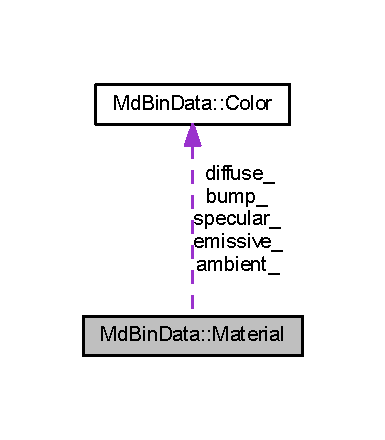
\includegraphics[width=185pt]{class_md_bin_data_1_1_material__coll__graph}
\end{center}
\end{figure}
\subsection*{クラス}
\begin{DoxyCompactItemize}
\item 
class \mbox{\hyperlink{class_md_bin_data_1_1_material_1_1_texture}{Texture}}
\begin{DoxyCompactList}\small\item\em テクスチャ\+Class \end{DoxyCompactList}\end{DoxyCompactItemize}
\subsection*{公開メンバ関数}
\begin{DoxyCompactItemize}
\item 
std\+::string $\ast$ \mbox{\hyperlink{class_md_bin_data_1_1_material_abaa620135fd033cce415e7c949e9a4b6}{getp\+Name}} ()
\begin{DoxyCompactList}\small\item\em 名前取得関数 \end{DoxyCompactList}\item 
\mbox{\hyperlink{class_md_bin_data_1_1_color}{Color}} $\ast$ \mbox{\hyperlink{class_md_bin_data_1_1_material_a5de4c3bff10499fb4fb861b7a13b6180}{getp\+Ambient}} ()
\begin{DoxyCompactList}\small\item\em アンビエント取得関数 \end{DoxyCompactList}\item 
\mbox{\hyperlink{class_md_bin_data_1_1_color}{Color}} $\ast$ \mbox{\hyperlink{class_md_bin_data_1_1_material_a3a66da1fbf79515b1bdff35b0278eb19}{getp\+Diffuse}} ()
\begin{DoxyCompactList}\small\item\em ディフューズ取得関数 \end{DoxyCompactList}\item 
\mbox{\hyperlink{class_md_bin_data_1_1_color}{Color}} $\ast$ \mbox{\hyperlink{class_md_bin_data_1_1_material_aa486af195c8862860ec61245e3933a64}{getp\+Emissive}} ()
\begin{DoxyCompactList}\small\item\em エミッション取得関数 \end{DoxyCompactList}\item 
\mbox{\hyperlink{class_md_bin_data_1_1_color}{Color}} $\ast$ \mbox{\hyperlink{class_md_bin_data_1_1_material_aec6d9f8f6c8e733c9165d39eebd55cc1}{getp\+Bump}} ()
\begin{DoxyCompactList}\small\item\em バンプ取得関数 \end{DoxyCompactList}\item 
float $\ast$ \mbox{\hyperlink{class_md_bin_data_1_1_material_a93eee0080dcebaa2f75fdfd6fc353ce0}{getp\+Transparent}} ()
\begin{DoxyCompactList}\small\item\em トランスペアレント取得関数 \end{DoxyCompactList}\item 
\mbox{\hyperlink{class_md_bin_data_1_1_color}{Color}} $\ast$ \mbox{\hyperlink{class_md_bin_data_1_1_material_a3dd95902f709e30a346dbc095e0eb900}{getp\+Specular}} ()
\begin{DoxyCompactList}\small\item\em スペキュラ取得関数 \end{DoxyCompactList}\item 
float $\ast$ \mbox{\hyperlink{class_md_bin_data_1_1_material_a2fad1db40f8d9466ac87be3782149104}{getp\+Power}} ()
\begin{DoxyCompactList}\small\item\em パワー取得関数 \end{DoxyCompactList}\item 
float $\ast$ \mbox{\hyperlink{class_md_bin_data_1_1_material_aa060a0f3fa72b5cfeef427c5a529e259}{getp\+Reflection}} ()
\begin{DoxyCompactList}\small\item\em リフレクション取得関数 \end{DoxyCompactList}\item 
int \mbox{\hyperlink{class_md_bin_data_1_1_material_a9ac4c6f4a97143645a1b5c78d321ba71}{get\+Texture\+Array\+Size}} ()
\begin{DoxyCompactList}\small\item\em テクスチャ配列サイズ取得関数 \end{DoxyCompactList}\item 
\mbox{\hyperlink{class_md_bin_data_1_1_material_1_1_texture}{Texture}} $\ast$ \mbox{\hyperlink{class_md_bin_data_1_1_material_a51888aa2e18d1d191818cad0ee07f45d}{getp\+Texture}} (int index)
\begin{DoxyCompactList}\small\item\em テクスチャ取得関数 \end{DoxyCompactList}\item 
void \mbox{\hyperlink{class_md_bin_data_1_1_material_a052ceb2c797f8a24c89d988510e874ae}{Release\+Texture\+Array}} ()
\begin{DoxyCompactList}\small\item\em テクスチャ解放関数 \end{DoxyCompactList}\item 
void \mbox{\hyperlink{class_md_bin_data_1_1_material_a8d6a7d5c0f7f11d84a155846c467a580}{Add\+Texture\+Array}} (\mbox{\hyperlink{class_md_bin_data_1_1_material_1_1_texture}{Texture}} $\ast$texture)
\begin{DoxyCompactList}\small\item\em テクスチャ配列追加関数 \end{DoxyCompactList}\end{DoxyCompactItemize}
\subsection*{非公開メンバ関数}
\begin{DoxyCompactItemize}
\item 
{\footnotesize template$<$class Archive $>$ }\\void \mbox{\hyperlink{class_md_bin_data_1_1_material_a5c3a4ba9a609aedbbaee7e0590ea27fc}{serialize}} (Archive \&archive, const unsigned version)
\end{DoxyCompactItemize}
\subsection*{非公開変数類}
\begin{DoxyCompactItemize}
\item 
std\+::string \mbox{\hyperlink{class_md_bin_data_1_1_material_a313cb12160a6bba5bee24cbae74ed091}{name\+\_\+}}
\begin{DoxyCompactList}\small\item\em 名前 \end{DoxyCompactList}\item 
\mbox{\hyperlink{class_md_bin_data_1_1_color}{Color}} \mbox{\hyperlink{class_md_bin_data_1_1_material_a1c102b19537a444f94e541015e3ac7f5}{ambient\+\_\+}}
\begin{DoxyCompactList}\small\item\em アンビエント(環境光) \end{DoxyCompactList}\item 
\mbox{\hyperlink{class_md_bin_data_1_1_color}{Color}} \mbox{\hyperlink{class_md_bin_data_1_1_material_a59cadfc22f9b91655f01414dc16f3e16}{diffuse\+\_\+}}
\begin{DoxyCompactList}\small\item\em ディヒューズ(拡散反射光) \end{DoxyCompactList}\item 
\mbox{\hyperlink{class_md_bin_data_1_1_color}{Color}} \mbox{\hyperlink{class_md_bin_data_1_1_material_aa38e2516efa84118397c533ff3e9b223}{emissive\+\_\+}}
\begin{DoxyCompactList}\small\item\em エミッシブ(放射光) \end{DoxyCompactList}\item 
\mbox{\hyperlink{class_md_bin_data_1_1_color}{Color}} \mbox{\hyperlink{class_md_bin_data_1_1_material_a210d4e9c5d3bdba5144086bfb792eca5}{bump\+\_\+}}
\begin{DoxyCompactList}\small\item\em バンプ(凹凸具合) \end{DoxyCompactList}\item 
float \mbox{\hyperlink{class_md_bin_data_1_1_material_a1d6d026a2e515d99c43bce457a99fb58}{transparent\+\_\+}}
\begin{DoxyCompactList}\small\item\em トランスペアレント(透過度) \end{DoxyCompactList}\item 
\mbox{\hyperlink{class_md_bin_data_1_1_color}{Color}} \mbox{\hyperlink{class_md_bin_data_1_1_material_a00c16d1b0970a1bfac1cbf5ae02511d4}{specular\+\_\+}}
\begin{DoxyCompactList}\small\item\em スペキュラ(鏡面反射) \end{DoxyCompactList}\item 
float \mbox{\hyperlink{class_md_bin_data_1_1_material_a5b8feee785a823f459b61c49da74441a}{power\+\_\+}}
\begin{DoxyCompactList}\small\item\em パワー(スペキュラの減衰強度) \end{DoxyCompactList}\item 
float \mbox{\hyperlink{class_md_bin_data_1_1_material_ac33b9c6e70a1eb229007e6c4f9c94712}{reflection\+\_\+}}
\begin{DoxyCompactList}\small\item\em リフレクション(反射強度) \end{DoxyCompactList}\item 
std\+::vector$<$ \mbox{\hyperlink{class_md_bin_data_1_1_material_1_1_texture}{Texture}} $\ast$ $>$ \mbox{\hyperlink{class_md_bin_data_1_1_material_ad5872731e44ecb8de180ccafa689bc6a}{texture\+\_\+array\+\_\+}}
\begin{DoxyCompactList}\small\item\em テクスチャ配列 \end{DoxyCompactList}\end{DoxyCompactItemize}
\subsection*{フレンド}
\begin{DoxyCompactItemize}
\item 
class \mbox{\hyperlink{class_md_bin_data_1_1_material_ac98d07dd8f7b70e16ccb9a01abf56b9c}{boost\+::serialization\+::access}}
\begin{DoxyCompactList}\small\item\em シリアライズ(I/O)関数 \end{DoxyCompactList}\end{DoxyCompactItemize}


\subsection{詳解}
マテリアル\+Class 

マテリアルの\+Class 

 Md\+Bin\+Data.\+h の 302 行目に定義があります。



\subsection{関数詳解}
\mbox{\Hypertarget{class_md_bin_data_1_1_material_a8d6a7d5c0f7f11d84a155846c467a580}\label{class_md_bin_data_1_1_material_a8d6a7d5c0f7f11d84a155846c467a580}} 
\index{Md\+Bin\+Data\+::\+Material@{Md\+Bin\+Data\+::\+Material}!Add\+Texture\+Array@{Add\+Texture\+Array}}
\index{Add\+Texture\+Array@{Add\+Texture\+Array}!Md\+Bin\+Data\+::\+Material@{Md\+Bin\+Data\+::\+Material}}
\subsubsection{\texorpdfstring{Add\+Texture\+Array()}{AddTextureArray()}}
{\footnotesize\ttfamily void Md\+Bin\+Data\+::\+Material\+::\+Add\+Texture\+Array (\begin{DoxyParamCaption}\item[{\mbox{\hyperlink{class_md_bin_data_1_1_material_1_1_texture}{Texture}} $\ast$}]{texture }\end{DoxyParamCaption})}



テクスチャ配列追加関数 


\begin{DoxyParams}{引数}
{\em $\ast$texture} & テクスチャ \\
\hline
\end{DoxyParams}

\begin{DoxyRetVals}{戻り値}
{\em void} & なし \\
\hline
\end{DoxyRetVals}


 Md\+Bin\+Data.\+cpp の 545 行目に定義があります。

\mbox{\Hypertarget{class_md_bin_data_1_1_material_a5de4c3bff10499fb4fb861b7a13b6180}\label{class_md_bin_data_1_1_material_a5de4c3bff10499fb4fb861b7a13b6180}} 
\index{Md\+Bin\+Data\+::\+Material@{Md\+Bin\+Data\+::\+Material}!getp\+Ambient@{getp\+Ambient}}
\index{getp\+Ambient@{getp\+Ambient}!Md\+Bin\+Data\+::\+Material@{Md\+Bin\+Data\+::\+Material}}
\subsubsection{\texorpdfstring{getp\+Ambient()}{getpAmbient()}}
{\footnotesize\ttfamily \mbox{\hyperlink{class_md_bin_data_1_1_color}{Md\+Bin\+Data\+::\+Color}} $\ast$ Md\+Bin\+Data\+::\+Material\+::getp\+Ambient (\begin{DoxyParamCaption}{ }\end{DoxyParamCaption})}



アンビエント取得関数 


\begin{DoxyParams}{引数}
{\em void} & なし \\
\hline
\end{DoxyParams}

\begin{DoxyRetVals}{戻り値}
{\em Color$\ast$} & アンビエント \\
\hline
\end{DoxyRetVals}


 Md\+Bin\+Data.\+cpp の 152 行目に定義があります。

\mbox{\Hypertarget{class_md_bin_data_1_1_material_aec6d9f8f6c8e733c9165d39eebd55cc1}\label{class_md_bin_data_1_1_material_aec6d9f8f6c8e733c9165d39eebd55cc1}} 
\index{Md\+Bin\+Data\+::\+Material@{Md\+Bin\+Data\+::\+Material}!getp\+Bump@{getp\+Bump}}
\index{getp\+Bump@{getp\+Bump}!Md\+Bin\+Data\+::\+Material@{Md\+Bin\+Data\+::\+Material}}
\subsubsection{\texorpdfstring{getp\+Bump()}{getpBump()}}
{\footnotesize\ttfamily \mbox{\hyperlink{class_md_bin_data_1_1_color}{Md\+Bin\+Data\+::\+Color}} $\ast$ Md\+Bin\+Data\+::\+Material\+::getp\+Bump (\begin{DoxyParamCaption}{ }\end{DoxyParamCaption})}



バンプ取得関数 


\begin{DoxyParams}{引数}
{\em void} & なし \\
\hline
\end{DoxyParams}

\begin{DoxyRetVals}{戻り値}
{\em Color$\ast$} & バンプ \\
\hline
\end{DoxyRetVals}


 Md\+Bin\+Data.\+cpp の 173 行目に定義があります。

\mbox{\Hypertarget{class_md_bin_data_1_1_material_a3a66da1fbf79515b1bdff35b0278eb19}\label{class_md_bin_data_1_1_material_a3a66da1fbf79515b1bdff35b0278eb19}} 
\index{Md\+Bin\+Data\+::\+Material@{Md\+Bin\+Data\+::\+Material}!getp\+Diffuse@{getp\+Diffuse}}
\index{getp\+Diffuse@{getp\+Diffuse}!Md\+Bin\+Data\+::\+Material@{Md\+Bin\+Data\+::\+Material}}
\subsubsection{\texorpdfstring{getp\+Diffuse()}{getpDiffuse()}}
{\footnotesize\ttfamily \mbox{\hyperlink{class_md_bin_data_1_1_color}{Md\+Bin\+Data\+::\+Color}} $\ast$ Md\+Bin\+Data\+::\+Material\+::getp\+Diffuse (\begin{DoxyParamCaption}{ }\end{DoxyParamCaption})}



ディフューズ取得関数 


\begin{DoxyParams}{引数}
{\em void} & なし \\
\hline
\end{DoxyParams}

\begin{DoxyRetVals}{戻り値}
{\em Color$\ast$} & ディフューズ \\
\hline
\end{DoxyRetVals}


 Md\+Bin\+Data.\+cpp の 159 行目に定義があります。

\mbox{\Hypertarget{class_md_bin_data_1_1_material_aa486af195c8862860ec61245e3933a64}\label{class_md_bin_data_1_1_material_aa486af195c8862860ec61245e3933a64}} 
\index{Md\+Bin\+Data\+::\+Material@{Md\+Bin\+Data\+::\+Material}!getp\+Emissive@{getp\+Emissive}}
\index{getp\+Emissive@{getp\+Emissive}!Md\+Bin\+Data\+::\+Material@{Md\+Bin\+Data\+::\+Material}}
\subsubsection{\texorpdfstring{getp\+Emissive()}{getpEmissive()}}
{\footnotesize\ttfamily \mbox{\hyperlink{class_md_bin_data_1_1_color}{Md\+Bin\+Data\+::\+Color}} $\ast$ Md\+Bin\+Data\+::\+Material\+::getp\+Emissive (\begin{DoxyParamCaption}{ }\end{DoxyParamCaption})}



エミッション取得関数 


\begin{DoxyParams}{引数}
{\em void} & なし \\
\hline
\end{DoxyParams}

\begin{DoxyRetVals}{戻り値}
{\em Color$\ast$} & エミッション \\
\hline
\end{DoxyRetVals}


 Md\+Bin\+Data.\+cpp の 166 行目に定義があります。

\mbox{\Hypertarget{class_md_bin_data_1_1_material_abaa620135fd033cce415e7c949e9a4b6}\label{class_md_bin_data_1_1_material_abaa620135fd033cce415e7c949e9a4b6}} 
\index{Md\+Bin\+Data\+::\+Material@{Md\+Bin\+Data\+::\+Material}!getp\+Name@{getp\+Name}}
\index{getp\+Name@{getp\+Name}!Md\+Bin\+Data\+::\+Material@{Md\+Bin\+Data\+::\+Material}}
\subsubsection{\texorpdfstring{getp\+Name()}{getpName()}}
{\footnotesize\ttfamily std\+::string $\ast$ Md\+Bin\+Data\+::\+Material\+::getp\+Name (\begin{DoxyParamCaption}{ }\end{DoxyParamCaption})}



名前取得関数 


\begin{DoxyParams}{引数}
{\em void} & なし \\
\hline
\end{DoxyParams}

\begin{DoxyRetVals}{戻り値}
{\em std\+::string$\ast$} & 名前 \\
\hline
\end{DoxyRetVals}


 Md\+Bin\+Data.\+cpp の 145 行目に定義があります。

\mbox{\Hypertarget{class_md_bin_data_1_1_material_a2fad1db40f8d9466ac87be3782149104}\label{class_md_bin_data_1_1_material_a2fad1db40f8d9466ac87be3782149104}} 
\index{Md\+Bin\+Data\+::\+Material@{Md\+Bin\+Data\+::\+Material}!getp\+Power@{getp\+Power}}
\index{getp\+Power@{getp\+Power}!Md\+Bin\+Data\+::\+Material@{Md\+Bin\+Data\+::\+Material}}
\subsubsection{\texorpdfstring{getp\+Power()}{getpPower()}}
{\footnotesize\ttfamily float $\ast$ Md\+Bin\+Data\+::\+Material\+::getp\+Power (\begin{DoxyParamCaption}{ }\end{DoxyParamCaption})}



パワー取得関数 


\begin{DoxyParams}{引数}
{\em void} & なし \\
\hline
\end{DoxyParams}

\begin{DoxyRetVals}{戻り値}
{\em float$\ast$} & パワー \\
\hline
\end{DoxyRetVals}


 Md\+Bin\+Data.\+cpp の 194 行目に定義があります。

\mbox{\Hypertarget{class_md_bin_data_1_1_material_aa060a0f3fa72b5cfeef427c5a529e259}\label{class_md_bin_data_1_1_material_aa060a0f3fa72b5cfeef427c5a529e259}} 
\index{Md\+Bin\+Data\+::\+Material@{Md\+Bin\+Data\+::\+Material}!getp\+Reflection@{getp\+Reflection}}
\index{getp\+Reflection@{getp\+Reflection}!Md\+Bin\+Data\+::\+Material@{Md\+Bin\+Data\+::\+Material}}
\subsubsection{\texorpdfstring{getp\+Reflection()}{getpReflection()}}
{\footnotesize\ttfamily float $\ast$ Md\+Bin\+Data\+::\+Material\+::getp\+Reflection (\begin{DoxyParamCaption}{ }\end{DoxyParamCaption})}



リフレクション取得関数 


\begin{DoxyParams}{引数}
{\em void} & なし \\
\hline
\end{DoxyParams}

\begin{DoxyRetVals}{戻り値}
{\em float$\ast$} & リフレクション \\
\hline
\end{DoxyRetVals}


 Md\+Bin\+Data.\+cpp の 201 行目に定義があります。

\mbox{\Hypertarget{class_md_bin_data_1_1_material_a3dd95902f709e30a346dbc095e0eb900}\label{class_md_bin_data_1_1_material_a3dd95902f709e30a346dbc095e0eb900}} 
\index{Md\+Bin\+Data\+::\+Material@{Md\+Bin\+Data\+::\+Material}!getp\+Specular@{getp\+Specular}}
\index{getp\+Specular@{getp\+Specular}!Md\+Bin\+Data\+::\+Material@{Md\+Bin\+Data\+::\+Material}}
\subsubsection{\texorpdfstring{getp\+Specular()}{getpSpecular()}}
{\footnotesize\ttfamily \mbox{\hyperlink{class_md_bin_data_1_1_color}{Md\+Bin\+Data\+::\+Color}} $\ast$ Md\+Bin\+Data\+::\+Material\+::getp\+Specular (\begin{DoxyParamCaption}{ }\end{DoxyParamCaption})}



スペキュラ取得関数 


\begin{DoxyParams}{引数}
{\em void} & なし \\
\hline
\end{DoxyParams}

\begin{DoxyRetVals}{戻り値}
{\em Color$\ast$} & スペキュラー \\
\hline
\end{DoxyRetVals}


 Md\+Bin\+Data.\+cpp の 187 行目に定義があります。

\mbox{\Hypertarget{class_md_bin_data_1_1_material_a51888aa2e18d1d191818cad0ee07f45d}\label{class_md_bin_data_1_1_material_a51888aa2e18d1d191818cad0ee07f45d}} 
\index{Md\+Bin\+Data\+::\+Material@{Md\+Bin\+Data\+::\+Material}!getp\+Texture@{getp\+Texture}}
\index{getp\+Texture@{getp\+Texture}!Md\+Bin\+Data\+::\+Material@{Md\+Bin\+Data\+::\+Material}}
\subsubsection{\texorpdfstring{getp\+Texture()}{getpTexture()}}
{\footnotesize\ttfamily \mbox{\hyperlink{class_md_bin_data_1_1_material_1_1_texture}{Md\+Bin\+Data\+::\+Material\+::\+Texture}} $\ast$ Md\+Bin\+Data\+::\+Material\+::getp\+Texture (\begin{DoxyParamCaption}\item[{int}]{index }\end{DoxyParamCaption})}



テクスチャ取得関数 


\begin{DoxyParams}{引数}
{\em index} & インデックス \\
\hline
\end{DoxyParams}

\begin{DoxyRetVals}{戻り値}
{\em \mbox{\hyperlink{class_md_bin_data_1_1_material_1_1_texture}{Texture}}} & テクスチャ \\
\hline
\end{DoxyRetVals}


 Md\+Bin\+Data.\+cpp の 215 行目に定義があります。

\mbox{\Hypertarget{class_md_bin_data_1_1_material_a93eee0080dcebaa2f75fdfd6fc353ce0}\label{class_md_bin_data_1_1_material_a93eee0080dcebaa2f75fdfd6fc353ce0}} 
\index{Md\+Bin\+Data\+::\+Material@{Md\+Bin\+Data\+::\+Material}!getp\+Transparent@{getp\+Transparent}}
\index{getp\+Transparent@{getp\+Transparent}!Md\+Bin\+Data\+::\+Material@{Md\+Bin\+Data\+::\+Material}}
\subsubsection{\texorpdfstring{getp\+Transparent()}{getpTransparent()}}
{\footnotesize\ttfamily float $\ast$ Md\+Bin\+Data\+::\+Material\+::getp\+Transparent (\begin{DoxyParamCaption}{ }\end{DoxyParamCaption})}



トランスペアレント取得関数 


\begin{DoxyParams}{引数}
{\em void} & なし \\
\hline
\end{DoxyParams}

\begin{DoxyRetVals}{戻り値}
{\em float$\ast$} & トランスペアレント \\
\hline
\end{DoxyRetVals}


 Md\+Bin\+Data.\+cpp の 180 行目に定義があります。

\mbox{\Hypertarget{class_md_bin_data_1_1_material_a9ac4c6f4a97143645a1b5c78d321ba71}\label{class_md_bin_data_1_1_material_a9ac4c6f4a97143645a1b5c78d321ba71}} 
\index{Md\+Bin\+Data\+::\+Material@{Md\+Bin\+Data\+::\+Material}!get\+Texture\+Array\+Size@{get\+Texture\+Array\+Size}}
\index{get\+Texture\+Array\+Size@{get\+Texture\+Array\+Size}!Md\+Bin\+Data\+::\+Material@{Md\+Bin\+Data\+::\+Material}}
\subsubsection{\texorpdfstring{get\+Texture\+Array\+Size()}{getTextureArraySize()}}
{\footnotesize\ttfamily int Md\+Bin\+Data\+::\+Material\+::get\+Texture\+Array\+Size (\begin{DoxyParamCaption}{ }\end{DoxyParamCaption})}



テクスチャ配列サイズ取得関数 


\begin{DoxyParams}{引数}
{\em void} & なし \\
\hline
\end{DoxyParams}

\begin{DoxyRetVals}{戻り値}
{\em int} & サイズ \\
\hline
\end{DoxyRetVals}


 Md\+Bin\+Data.\+cpp の 208 行目に定義があります。

\mbox{\Hypertarget{class_md_bin_data_1_1_material_a052ceb2c797f8a24c89d988510e874ae}\label{class_md_bin_data_1_1_material_a052ceb2c797f8a24c89d988510e874ae}} 
\index{Md\+Bin\+Data\+::\+Material@{Md\+Bin\+Data\+::\+Material}!Release\+Texture\+Array@{Release\+Texture\+Array}}
\index{Release\+Texture\+Array@{Release\+Texture\+Array}!Md\+Bin\+Data\+::\+Material@{Md\+Bin\+Data\+::\+Material}}
\subsubsection{\texorpdfstring{Release\+Texture\+Array()}{ReleaseTextureArray()}}
{\footnotesize\ttfamily void Md\+Bin\+Data\+::\+Material\+::\+Release\+Texture\+Array (\begin{DoxyParamCaption}{ }\end{DoxyParamCaption})}



テクスチャ解放関数 


\begin{DoxyParams}{引数}
{\em void} & なし \\
\hline
\end{DoxyParams}

\begin{DoxyRetVals}{戻り値}
{\em void} & なし \\
\hline
\end{DoxyRetVals}


 Md\+Bin\+Data.\+cpp の 533 行目に定義があります。

\mbox{\Hypertarget{class_md_bin_data_1_1_material_a5c3a4ba9a609aedbbaee7e0590ea27fc}\label{class_md_bin_data_1_1_material_a5c3a4ba9a609aedbbaee7e0590ea27fc}} 
\index{Md\+Bin\+Data\+::\+Material@{Md\+Bin\+Data\+::\+Material}!serialize@{serialize}}
\index{serialize@{serialize}!Md\+Bin\+Data\+::\+Material@{Md\+Bin\+Data\+::\+Material}}
\subsubsection{\texorpdfstring{serialize()}{serialize()}}
{\footnotesize\ttfamily template$<$class Archive $>$ \\
void Md\+Bin\+Data\+::\+Material\+::serialize (\begin{DoxyParamCaption}\item[{Archive \&}]{archive,  }\item[{const unsigned}]{version }\end{DoxyParamCaption})\hspace{0.3cm}{\ttfamily [inline]}, {\ttfamily [private]}}



 Md\+Bin\+Data.\+h の 526 行目に定義があります。



\subsection{フレンドと関連関数の詳解}
\mbox{\Hypertarget{class_md_bin_data_1_1_material_ac98d07dd8f7b70e16ccb9a01abf56b9c}\label{class_md_bin_data_1_1_material_ac98d07dd8f7b70e16ccb9a01abf56b9c}} 
\index{Md\+Bin\+Data\+::\+Material@{Md\+Bin\+Data\+::\+Material}!boost\+::serialization\+::access@{boost\+::serialization\+::access}}
\index{boost\+::serialization\+::access@{boost\+::serialization\+::access}!Md\+Bin\+Data\+::\+Material@{Md\+Bin\+Data\+::\+Material}}
\subsubsection{\texorpdfstring{boost\+::serialization\+::access}{boost::serialization::access}}
{\footnotesize\ttfamily friend class boost\+::serialization\+::access\hspace{0.3cm}{\ttfamily [friend]}}



シリアライズ(I/O)関数 


\begin{DoxyParams}{引数}
{\em archive} & アーカイブ用クラス \\
\hline
{\em version} & バージョン \\
\hline
\end{DoxyParams}

\begin{DoxyRetVals}{戻り値}
{\em void} & なし \\
\hline
\end{DoxyRetVals}


 Md\+Bin\+Data.\+h の 524 行目に定義があります。



\subsection{メンバ詳解}
\mbox{\Hypertarget{class_md_bin_data_1_1_material_a1c102b19537a444f94e541015e3ac7f5}\label{class_md_bin_data_1_1_material_a1c102b19537a444f94e541015e3ac7f5}} 
\index{Md\+Bin\+Data\+::\+Material@{Md\+Bin\+Data\+::\+Material}!ambient\+\_\+@{ambient\+\_\+}}
\index{ambient\+\_\+@{ambient\+\_\+}!Md\+Bin\+Data\+::\+Material@{Md\+Bin\+Data\+::\+Material}}
\subsubsection{\texorpdfstring{ambient\+\_\+}{ambient\_}}
{\footnotesize\ttfamily \mbox{\hyperlink{class_md_bin_data_1_1_color}{Color}} Md\+Bin\+Data\+::\+Material\+::ambient\+\_\+\hspace{0.3cm}{\ttfamily [private]}}



アンビエント(環境光) 



 Md\+Bin\+Data.\+h の 388 行目に定義があります。

\mbox{\Hypertarget{class_md_bin_data_1_1_material_a210d4e9c5d3bdba5144086bfb792eca5}\label{class_md_bin_data_1_1_material_a210d4e9c5d3bdba5144086bfb792eca5}} 
\index{Md\+Bin\+Data\+::\+Material@{Md\+Bin\+Data\+::\+Material}!bump\+\_\+@{bump\+\_\+}}
\index{bump\+\_\+@{bump\+\_\+}!Md\+Bin\+Data\+::\+Material@{Md\+Bin\+Data\+::\+Material}}
\subsubsection{\texorpdfstring{bump\+\_\+}{bump\_}}
{\footnotesize\ttfamily \mbox{\hyperlink{class_md_bin_data_1_1_color}{Color}} Md\+Bin\+Data\+::\+Material\+::bump\+\_\+\hspace{0.3cm}{\ttfamily [private]}}



バンプ(凹凸具合) 



 Md\+Bin\+Data.\+h の 391 行目に定義があります。

\mbox{\Hypertarget{class_md_bin_data_1_1_material_a59cadfc22f9b91655f01414dc16f3e16}\label{class_md_bin_data_1_1_material_a59cadfc22f9b91655f01414dc16f3e16}} 
\index{Md\+Bin\+Data\+::\+Material@{Md\+Bin\+Data\+::\+Material}!diffuse\+\_\+@{diffuse\+\_\+}}
\index{diffuse\+\_\+@{diffuse\+\_\+}!Md\+Bin\+Data\+::\+Material@{Md\+Bin\+Data\+::\+Material}}
\subsubsection{\texorpdfstring{diffuse\+\_\+}{diffuse\_}}
{\footnotesize\ttfamily \mbox{\hyperlink{class_md_bin_data_1_1_color}{Color}} Md\+Bin\+Data\+::\+Material\+::diffuse\+\_\+\hspace{0.3cm}{\ttfamily [private]}}



ディヒューズ(拡散反射光) 



 Md\+Bin\+Data.\+h の 389 行目に定義があります。

\mbox{\Hypertarget{class_md_bin_data_1_1_material_aa38e2516efa84118397c533ff3e9b223}\label{class_md_bin_data_1_1_material_aa38e2516efa84118397c533ff3e9b223}} 
\index{Md\+Bin\+Data\+::\+Material@{Md\+Bin\+Data\+::\+Material}!emissive\+\_\+@{emissive\+\_\+}}
\index{emissive\+\_\+@{emissive\+\_\+}!Md\+Bin\+Data\+::\+Material@{Md\+Bin\+Data\+::\+Material}}
\subsubsection{\texorpdfstring{emissive\+\_\+}{emissive\_}}
{\footnotesize\ttfamily \mbox{\hyperlink{class_md_bin_data_1_1_color}{Color}} Md\+Bin\+Data\+::\+Material\+::emissive\+\_\+\hspace{0.3cm}{\ttfamily [private]}}



エミッシブ(放射光) 



 Md\+Bin\+Data.\+h の 390 行目に定義があります。

\mbox{\Hypertarget{class_md_bin_data_1_1_material_a313cb12160a6bba5bee24cbae74ed091}\label{class_md_bin_data_1_1_material_a313cb12160a6bba5bee24cbae74ed091}} 
\index{Md\+Bin\+Data\+::\+Material@{Md\+Bin\+Data\+::\+Material}!name\+\_\+@{name\+\_\+}}
\index{name\+\_\+@{name\+\_\+}!Md\+Bin\+Data\+::\+Material@{Md\+Bin\+Data\+::\+Material}}
\subsubsection{\texorpdfstring{name\+\_\+}{name\_}}
{\footnotesize\ttfamily std\+::string Md\+Bin\+Data\+::\+Material\+::name\+\_\+\hspace{0.3cm}{\ttfamily [private]}}



名前 



 Md\+Bin\+Data.\+h の 387 行目に定義があります。

\mbox{\Hypertarget{class_md_bin_data_1_1_material_a5b8feee785a823f459b61c49da74441a}\label{class_md_bin_data_1_1_material_a5b8feee785a823f459b61c49da74441a}} 
\index{Md\+Bin\+Data\+::\+Material@{Md\+Bin\+Data\+::\+Material}!power\+\_\+@{power\+\_\+}}
\index{power\+\_\+@{power\+\_\+}!Md\+Bin\+Data\+::\+Material@{Md\+Bin\+Data\+::\+Material}}
\subsubsection{\texorpdfstring{power\+\_\+}{power\_}}
{\footnotesize\ttfamily float Md\+Bin\+Data\+::\+Material\+::power\+\_\+\hspace{0.3cm}{\ttfamily [private]}}



パワー(スペキュラの減衰強度) 



 Md\+Bin\+Data.\+h の 394 行目に定義があります。

\mbox{\Hypertarget{class_md_bin_data_1_1_material_ac33b9c6e70a1eb229007e6c4f9c94712}\label{class_md_bin_data_1_1_material_ac33b9c6e70a1eb229007e6c4f9c94712}} 
\index{Md\+Bin\+Data\+::\+Material@{Md\+Bin\+Data\+::\+Material}!reflection\+\_\+@{reflection\+\_\+}}
\index{reflection\+\_\+@{reflection\+\_\+}!Md\+Bin\+Data\+::\+Material@{Md\+Bin\+Data\+::\+Material}}
\subsubsection{\texorpdfstring{reflection\+\_\+}{reflection\_}}
{\footnotesize\ttfamily float Md\+Bin\+Data\+::\+Material\+::reflection\+\_\+\hspace{0.3cm}{\ttfamily [private]}}



リフレクション(反射強度) 



 Md\+Bin\+Data.\+h の 395 行目に定義があります。

\mbox{\Hypertarget{class_md_bin_data_1_1_material_a00c16d1b0970a1bfac1cbf5ae02511d4}\label{class_md_bin_data_1_1_material_a00c16d1b0970a1bfac1cbf5ae02511d4}} 
\index{Md\+Bin\+Data\+::\+Material@{Md\+Bin\+Data\+::\+Material}!specular\+\_\+@{specular\+\_\+}}
\index{specular\+\_\+@{specular\+\_\+}!Md\+Bin\+Data\+::\+Material@{Md\+Bin\+Data\+::\+Material}}
\subsubsection{\texorpdfstring{specular\+\_\+}{specular\_}}
{\footnotesize\ttfamily \mbox{\hyperlink{class_md_bin_data_1_1_color}{Color}} Md\+Bin\+Data\+::\+Material\+::specular\+\_\+\hspace{0.3cm}{\ttfamily [private]}}



スペキュラ(鏡面反射) 



 Md\+Bin\+Data.\+h の 393 行目に定義があります。

\mbox{\Hypertarget{class_md_bin_data_1_1_material_ad5872731e44ecb8de180ccafa689bc6a}\label{class_md_bin_data_1_1_material_ad5872731e44ecb8de180ccafa689bc6a}} 
\index{Md\+Bin\+Data\+::\+Material@{Md\+Bin\+Data\+::\+Material}!texture\+\_\+array\+\_\+@{texture\+\_\+array\+\_\+}}
\index{texture\+\_\+array\+\_\+@{texture\+\_\+array\+\_\+}!Md\+Bin\+Data\+::\+Material@{Md\+Bin\+Data\+::\+Material}}
\subsubsection{\texorpdfstring{texture\+\_\+array\+\_\+}{texture\_array\_}}
{\footnotesize\ttfamily std\+::vector$<$\mbox{\hyperlink{class_md_bin_data_1_1_material_1_1_texture}{Texture}}$\ast$$>$ Md\+Bin\+Data\+::\+Material\+::texture\+\_\+array\+\_\+\hspace{0.3cm}{\ttfamily [private]}}



テクスチャ配列 



 Md\+Bin\+Data.\+h の 396 行目に定義があります。

\mbox{\Hypertarget{class_md_bin_data_1_1_material_a1d6d026a2e515d99c43bce457a99fb58}\label{class_md_bin_data_1_1_material_a1d6d026a2e515d99c43bce457a99fb58}} 
\index{Md\+Bin\+Data\+::\+Material@{Md\+Bin\+Data\+::\+Material}!transparent\+\_\+@{transparent\+\_\+}}
\index{transparent\+\_\+@{transparent\+\_\+}!Md\+Bin\+Data\+::\+Material@{Md\+Bin\+Data\+::\+Material}}
\subsubsection{\texorpdfstring{transparent\+\_\+}{transparent\_}}
{\footnotesize\ttfamily float Md\+Bin\+Data\+::\+Material\+::transparent\+\_\+\hspace{0.3cm}{\ttfamily [private]}}



トランスペアレント(透過度) 



 Md\+Bin\+Data.\+h の 392 行目に定義があります。



このクラス詳解は次のファイルから抽出されました\+:\begin{DoxyCompactItemize}
\item 
C\+:/\+H\+A\+L/\+P\+G関係/03\+\_\+作成プログラム/03\+\_\+\+H\+A\+L授業/就職作品/\+Fbx\+Converter/source/\+Md\+Bin\+Data/\mbox{\hyperlink{_md_bin_data_8h}{Md\+Bin\+Data.\+h}}\item 
C\+:/\+H\+A\+L/\+P\+G関係/03\+\_\+作成プログラム/03\+\_\+\+H\+A\+L授業/就職作品/\+Fbx\+Converter/source/\+Md\+Bin\+Data/\mbox{\hyperlink{_md_bin_data_8cpp}{Md\+Bin\+Data.\+cpp}}\end{DoxyCompactItemize}

\hypertarget{class_md_bin_data_1_1_matrix}{}\section{Md\+Bin\+Data\+:\+:Matrix クラス}
\label{class_md_bin_data_1_1_matrix}\index{Md\+Bin\+Data\+::\+Matrix@{Md\+Bin\+Data\+::\+Matrix}}


行列\+Class  




{\ttfamily \#include $<$Md\+Bin\+Data.\+h$>$}

\subsection*{公開メンバ関数}
\begin{DoxyCompactItemize}
\item 
float \mbox{\hyperlink{class_md_bin_data_1_1_matrix_a18fdeb0e8152f5f8a8ba8e8d64c925bf}{get\+Matrix\+Element}} (unsigned index0, unsigned index1)
\begin{DoxyCompactList}\small\item\em 配列要素取得関数 \end{DoxyCompactList}\item 
void \mbox{\hyperlink{class_md_bin_data_1_1_matrix_a0e5ff333aec5c3c27fb5b0d14e085b91}{set\+Matrix\+Element}} (float value, unsigned index0, unsigned index1)
\begin{DoxyCompactList}\small\item\em 配列要素設定関数 \end{DoxyCompactList}\end{DoxyCompactItemize}
\subsection*{静的公開変数類}
\begin{DoxyCompactItemize}
\item 
static const unsigned \mbox{\hyperlink{class_md_bin_data_1_1_matrix_adbf2f2e21df64ab4559b9c98b88a6c59}{A\+R\+R\+A\+Y\+\_\+\+W\+I\+D\+TH}} = 4
\item 
static const unsigned \mbox{\hyperlink{class_md_bin_data_1_1_matrix_a69ea4171a8c2fbf1728396463bfd9bc8}{A\+R\+R\+A\+Y\+\_\+\+H\+E\+I\+G\+HT}} = 4
\end{DoxyCompactItemize}
\subsection*{非公開メンバ関数}
\begin{DoxyCompactItemize}
\item 
{\footnotesize template$<$class Archive $>$ }\\void \mbox{\hyperlink{class_md_bin_data_1_1_matrix_a8494155c326062f5a4c7e2352b7c577d}{serialize}} (Archive \&archive, const unsigned version)
\end{DoxyCompactItemize}
\subsection*{非公開変数類}
\begin{DoxyCompactItemize}
\item 
float \mbox{\hyperlink{class_md_bin_data_1_1_matrix_a9b13d72966bb7b35e1c5acbfef92095f}{array\+\_\+}} \mbox{[}\mbox{\hyperlink{class_md_bin_data_1_1_matrix_a69ea4171a8c2fbf1728396463bfd9bc8}{A\+R\+R\+A\+Y\+\_\+\+H\+E\+I\+G\+HT}}\mbox{]}\mbox{[}\mbox{\hyperlink{class_md_bin_data_1_1_matrix_adbf2f2e21df64ab4559b9c98b88a6c59}{A\+R\+R\+A\+Y\+\_\+\+W\+I\+D\+TH}}\mbox{]}
\begin{DoxyCompactList}\small\item\em 4x4行列 \end{DoxyCompactList}\end{DoxyCompactItemize}
\subsection*{フレンド}
\begin{DoxyCompactItemize}
\item 
class \mbox{\hyperlink{class_md_bin_data_1_1_matrix_ac98d07dd8f7b70e16ccb9a01abf56b9c}{boost\+::serialization\+::access}}
\begin{DoxyCompactList}\small\item\em シリアライズ(I/O)関数 \end{DoxyCompactList}\end{DoxyCompactItemize}


\subsection{詳解}
行列\+Class 

行列の\+Class 

 Md\+Bin\+Data.\+h の 234 行目に定義があります。



\subsection{関数詳解}
\mbox{\Hypertarget{class_md_bin_data_1_1_matrix_a18fdeb0e8152f5f8a8ba8e8d64c925bf}\label{class_md_bin_data_1_1_matrix_a18fdeb0e8152f5f8a8ba8e8d64c925bf}} 
\index{Md\+Bin\+Data\+::\+Matrix@{Md\+Bin\+Data\+::\+Matrix}!get\+Matrix\+Element@{get\+Matrix\+Element}}
\index{get\+Matrix\+Element@{get\+Matrix\+Element}!Md\+Bin\+Data\+::\+Matrix@{Md\+Bin\+Data\+::\+Matrix}}
\subsubsection{\texorpdfstring{get\+Matrix\+Element()}{getMatrixElement()}}
{\footnotesize\ttfamily float Md\+Bin\+Data\+::\+Matrix\+::get\+Matrix\+Element (\begin{DoxyParamCaption}\item[{unsigned}]{index0,  }\item[{unsigned}]{index1 }\end{DoxyParamCaption})}



配列要素取得関数 


\begin{DoxyParams}{引数}
{\em index0} & 0番目のインデックス \\
\hline
{\em index1} & 1番目のインデックス \\
\hline
\end{DoxyParams}

\begin{DoxyRetVals}{戻り値}
{\em float} & 配列要素 \\
\hline
\end{DoxyRetVals}


 Md\+Bin\+Data.\+cpp の 117 行目に定義があります。

\mbox{\Hypertarget{class_md_bin_data_1_1_matrix_a8494155c326062f5a4c7e2352b7c577d}\label{class_md_bin_data_1_1_matrix_a8494155c326062f5a4c7e2352b7c577d}} 
\index{Md\+Bin\+Data\+::\+Matrix@{Md\+Bin\+Data\+::\+Matrix}!serialize@{serialize}}
\index{serialize@{serialize}!Md\+Bin\+Data\+::\+Matrix@{Md\+Bin\+Data\+::\+Matrix}}
\subsubsection{\texorpdfstring{serialize()}{serialize()}}
{\footnotesize\ttfamily template$<$class Archive $>$ \\
void Md\+Bin\+Data\+::\+Matrix\+::serialize (\begin{DoxyParamCaption}\item[{Archive \&}]{archive,  }\item[{const unsigned}]{version }\end{DoxyParamCaption})\hspace{0.3cm}{\ttfamily [inline]}, {\ttfamily [private]}}



 Md\+Bin\+Data.\+h の 288 行目に定義があります。

\mbox{\Hypertarget{class_md_bin_data_1_1_matrix_a0e5ff333aec5c3c27fb5b0d14e085b91}\label{class_md_bin_data_1_1_matrix_a0e5ff333aec5c3c27fb5b0d14e085b91}} 
\index{Md\+Bin\+Data\+::\+Matrix@{Md\+Bin\+Data\+::\+Matrix}!set\+Matrix\+Element@{set\+Matrix\+Element}}
\index{set\+Matrix\+Element@{set\+Matrix\+Element}!Md\+Bin\+Data\+::\+Matrix@{Md\+Bin\+Data\+::\+Matrix}}
\subsubsection{\texorpdfstring{set\+Matrix\+Element()}{setMatrixElement()}}
{\footnotesize\ttfamily void Md\+Bin\+Data\+::\+Matrix\+::set\+Matrix\+Element (\begin{DoxyParamCaption}\item[{float}]{value,  }\item[{unsigned}]{index0,  }\item[{unsigned}]{index1 }\end{DoxyParamCaption})}



配列要素設定関数 


\begin{DoxyParams}{引数}
{\em value} & 値 \\
\hline
{\em index0} & 0番目のインデックス \\
\hline
{\em index1} & 1番目のインデックス \\
\hline
\end{DoxyParams}

\begin{DoxyRetVals}{戻り値}
{\em void} & なし \\
\hline
\end{DoxyRetVals}


 Md\+Bin\+Data.\+cpp の 124 行目に定義があります。



\subsection{フレンドと関連関数の詳解}
\mbox{\Hypertarget{class_md_bin_data_1_1_matrix_ac98d07dd8f7b70e16ccb9a01abf56b9c}\label{class_md_bin_data_1_1_matrix_ac98d07dd8f7b70e16ccb9a01abf56b9c}} 
\index{Md\+Bin\+Data\+::\+Matrix@{Md\+Bin\+Data\+::\+Matrix}!boost\+::serialization\+::access@{boost\+::serialization\+::access}}
\index{boost\+::serialization\+::access@{boost\+::serialization\+::access}!Md\+Bin\+Data\+::\+Matrix@{Md\+Bin\+Data\+::\+Matrix}}
\subsubsection{\texorpdfstring{boost\+::serialization\+::access}{boost::serialization::access}}
{\footnotesize\ttfamily friend class boost\+::serialization\+::access\hspace{0.3cm}{\ttfamily [friend]}}



シリアライズ(I/O)関数 


\begin{DoxyParams}{引数}
{\em archive} & アーカイブ用クラス \\
\hline
{\em version} & バージョン \\
\hline
\end{DoxyParams}

\begin{DoxyRetVals}{戻り値}
{\em void} & なし \\
\hline
\end{DoxyRetVals}


 Md\+Bin\+Data.\+h の 286 行目に定義があります。



\subsection{メンバ詳解}
\mbox{\Hypertarget{class_md_bin_data_1_1_matrix_a9b13d72966bb7b35e1c5acbfef92095f}\label{class_md_bin_data_1_1_matrix_a9b13d72966bb7b35e1c5acbfef92095f}} 
\index{Md\+Bin\+Data\+::\+Matrix@{Md\+Bin\+Data\+::\+Matrix}!array\+\_\+@{array\+\_\+}}
\index{array\+\_\+@{array\+\_\+}!Md\+Bin\+Data\+::\+Matrix@{Md\+Bin\+Data\+::\+Matrix}}
\subsubsection{\texorpdfstring{array\+\_\+}{array\_}}
{\footnotesize\ttfamily float Md\+Bin\+Data\+::\+Matrix\+::array\+\_\+\mbox{[}\mbox{\hyperlink{class_md_bin_data_1_1_matrix_a69ea4171a8c2fbf1728396463bfd9bc8}{A\+R\+R\+A\+Y\+\_\+\+H\+E\+I\+G\+HT}}\mbox{]}\mbox{[}\mbox{\hyperlink{class_md_bin_data_1_1_matrix_adbf2f2e21df64ab4559b9c98b88a6c59}{A\+R\+R\+A\+Y\+\_\+\+W\+I\+D\+TH}}\mbox{]}\hspace{0.3cm}{\ttfamily [private]}}



4x4行列 



 Md\+Bin\+Data.\+h の 248 行目に定義があります。

\mbox{\Hypertarget{class_md_bin_data_1_1_matrix_a69ea4171a8c2fbf1728396463bfd9bc8}\label{class_md_bin_data_1_1_matrix_a69ea4171a8c2fbf1728396463bfd9bc8}} 
\index{Md\+Bin\+Data\+::\+Matrix@{Md\+Bin\+Data\+::\+Matrix}!A\+R\+R\+A\+Y\+\_\+\+H\+E\+I\+G\+HT@{A\+R\+R\+A\+Y\+\_\+\+H\+E\+I\+G\+HT}}
\index{A\+R\+R\+A\+Y\+\_\+\+H\+E\+I\+G\+HT@{A\+R\+R\+A\+Y\+\_\+\+H\+E\+I\+G\+HT}!Md\+Bin\+Data\+::\+Matrix@{Md\+Bin\+Data\+::\+Matrix}}
\subsubsection{\texorpdfstring{A\+R\+R\+A\+Y\+\_\+\+H\+E\+I\+G\+HT}{ARRAY\_HEIGHT}}
{\footnotesize\ttfamily const unsigned Md\+Bin\+Data\+::\+Matrix\+::\+A\+R\+R\+A\+Y\+\_\+\+H\+E\+I\+G\+HT = 4\hspace{0.3cm}{\ttfamily [static]}}



 Md\+Bin\+Data.\+h の 241 行目に定義があります。

\mbox{\Hypertarget{class_md_bin_data_1_1_matrix_adbf2f2e21df64ab4559b9c98b88a6c59}\label{class_md_bin_data_1_1_matrix_adbf2f2e21df64ab4559b9c98b88a6c59}} 
\index{Md\+Bin\+Data\+::\+Matrix@{Md\+Bin\+Data\+::\+Matrix}!A\+R\+R\+A\+Y\+\_\+\+W\+I\+D\+TH@{A\+R\+R\+A\+Y\+\_\+\+W\+I\+D\+TH}}
\index{A\+R\+R\+A\+Y\+\_\+\+W\+I\+D\+TH@{A\+R\+R\+A\+Y\+\_\+\+W\+I\+D\+TH}!Md\+Bin\+Data\+::\+Matrix@{Md\+Bin\+Data\+::\+Matrix}}
\subsubsection{\texorpdfstring{A\+R\+R\+A\+Y\+\_\+\+W\+I\+D\+TH}{ARRAY\_WIDTH}}
{\footnotesize\ttfamily const unsigned Md\+Bin\+Data\+::\+Matrix\+::\+A\+R\+R\+A\+Y\+\_\+\+W\+I\+D\+TH = 4\hspace{0.3cm}{\ttfamily [static]}}



 Md\+Bin\+Data.\+h の 240 行目に定義があります。



このクラス詳解は次のファイルから抽出されました\+:\begin{DoxyCompactItemize}
\item 
C\+:/\+H\+A\+L/\+P\+G関係/03\+\_\+作成プログラム/03\+\_\+\+H\+A\+L授業/就職作品/\+Fbx\+Converter/source/\+Md\+Bin\+Data/\mbox{\hyperlink{_md_bin_data_8h}{Md\+Bin\+Data.\+h}}\item 
C\+:/\+H\+A\+L/\+P\+G関係/03\+\_\+作成プログラム/03\+\_\+\+H\+A\+L授業/就職作品/\+Fbx\+Converter/source/\+Md\+Bin\+Data/\mbox{\hyperlink{_md_bin_data_8cpp}{Md\+Bin\+Data.\+cpp}}\end{DoxyCompactItemize}

\hypertarget{class_md_bin_data}{}\section{Md\+Bin\+Data クラス}
\label{class_md_bin_data}\index{Md\+Bin\+Data@{Md\+Bin\+Data}}


バイナリーモデルデータ\+Class  




{\ttfamily \#include $<$Md\+Bin\+Data.\+h$>$}

\subsection*{クラス}
\begin{DoxyCompactItemize}
\item 
class \mbox{\hyperlink{class_md_bin_data_1_1_color}{Color}}
\begin{DoxyCompactList}\small\item\em 色\+Class \end{DoxyCompactList}\item 
class \mbox{\hyperlink{class_md_bin_data_1_1_material}{Material}}
\begin{DoxyCompactList}\small\item\em マテリアル\+Class \end{DoxyCompactList}\item 
class \mbox{\hyperlink{class_md_bin_data_1_1_matrix}{Matrix}}
\begin{DoxyCompactList}\small\item\em 行列\+Class \end{DoxyCompactList}\item 
class \mbox{\hyperlink{class_md_bin_data_1_1_mesh}{Mesh}}
\begin{DoxyCompactList}\small\item\em メッシュ\+Class \end{DoxyCompactList}\item 
class \mbox{\hyperlink{class_md_bin_data_1_1_vector2}{Vector2}}
\begin{DoxyCompactList}\small\item\em ベクター2\+Class \end{DoxyCompactList}\item 
class \mbox{\hyperlink{class_md_bin_data_1_1_vector3}{Vector3}}
\begin{DoxyCompactList}\small\item\em ベクター3\+Class \end{DoxyCompactList}\end{DoxyCompactItemize}
\subsection*{公開メンバ関数}
\begin{DoxyCompactItemize}
\item 
int \mbox{\hyperlink{class_md_bin_data_a6aa476ad1bb36532609cf344d68a53d8}{get\+Mesh\+Array\+Size}} ()
\begin{DoxyCompactList}\small\item\em メッシュ配列サイズ取得関数 \end{DoxyCompactList}\item 
void \mbox{\hyperlink{class_md_bin_data_aa0e9c2a5db151909fbbf0c3ef41c4e25}{set\+Mesh\+Array\+Size}} (int value)
\begin{DoxyCompactList}\small\item\em メッシュ配列サイズ設定関数 \end{DoxyCompactList}\item 
\mbox{\hyperlink{class_md_bin_data_1_1_mesh}{Mesh}} $\ast$ \mbox{\hyperlink{class_md_bin_data_a8a5dfdabb48917851cea4faa7faf4e35}{getp\+Mesh}} (int index)
\begin{DoxyCompactList}\small\item\em メッシュ取得関数 \end{DoxyCompactList}\item 
int \mbox{\hyperlink{class_md_bin_data_aabed66d8e767c03ad946280048faf226}{get\+Material\+Array\+Size}} ()
\begin{DoxyCompactList}\small\item\em マテリアル配列サイズ取得関数 \end{DoxyCompactList}\item 
void \mbox{\hyperlink{class_md_bin_data_afe92da8866475459da756ecfb92e2683}{set\+Material\+Array\+Size}} (int value)
\begin{DoxyCompactList}\small\item\em マテリアル配列サイズ設定関数 \end{DoxyCompactList}\item 
\mbox{\hyperlink{class_md_bin_data_1_1_material}{Material}} $\ast$ \mbox{\hyperlink{class_md_bin_data_a10bca66286683a1031fc64307866270a}{getp\+Material}} (int index)
\begin{DoxyCompactList}\small\item\em マテリアル取得関数 \end{DoxyCompactList}\item 
int \mbox{\hyperlink{class_md_bin_data_a07857df021c7efa671fb1ed2f764903d}{get\+Animation\+Fram\+Num}} ()
\begin{DoxyCompactList}\small\item\em アニメーションフレーム数取得関数 \end{DoxyCompactList}\item 
void \mbox{\hyperlink{class_md_bin_data_a656893994f5197194cae842918090f59}{set\+Animation\+Fram\+Num}} (int value)
\begin{DoxyCompactList}\small\item\em アニメーションフレーム数設定関数 \end{DoxyCompactList}\item 
\mbox{\hyperlink{class_md_bin_data_a8a2fe0ddd94c58c37e513f19b94c044f}{$\sim$\+Md\+Bin\+Data}} ()
\begin{DoxyCompactList}\small\item\em デストラクタ関数 \end{DoxyCompactList}\end{DoxyCompactItemize}
\subsection*{静的公開メンバ関数}
\begin{DoxyCompactItemize}
\item 
static bool \mbox{\hyperlink{class_md_bin_data_a75fdc719dd711d95d3cd7519132a2ba4}{Inport\+Data}} (\mbox{\hyperlink{class_md_bin_data}{Md\+Bin\+Data}} $\ast$md\+\_\+bin\+\_\+data\+\_\+container, std\+::string file\+\_\+path)
\begin{DoxyCompactList}\small\item\em インポートデータ関数 \end{DoxyCompactList}\item 
static bool \mbox{\hyperlink{class_md_bin_data_aa9e3d4f176e966533640206296a222cd}{Export\+Data}} (\mbox{\hyperlink{class_md_bin_data}{Md\+Bin\+Data}} $\ast$md\+\_\+bin\+\_\+data\+\_\+container, std\+::string file\+\_\+path)
\begin{DoxyCompactList}\small\item\em エクスポートデータ関数 \end{DoxyCompactList}\end{DoxyCompactItemize}
\subsection*{非公開メンバ関数}
\begin{DoxyCompactItemize}
\item 
{\footnotesize template$<$class Archive $>$ }\\void \mbox{\hyperlink{class_md_bin_data_a3311ed96bf9545d30a9b08c6649078a9}{serialize}} (Archive \&archive, const unsigned version)
\end{DoxyCompactItemize}
\subsection*{非公開変数類}
\begin{DoxyCompactItemize}
\item 
std\+::vector$<$ \mbox{\hyperlink{class_md_bin_data_1_1_mesh}{Mesh}} $>$ \mbox{\hyperlink{class_md_bin_data_aefce3cdcd6dcdf388c936ade62c6b9fa}{mesh\+\_\+array\+\_\+}}
\begin{DoxyCompactList}\small\item\em メッシュ配列 \end{DoxyCompactList}\item 
std\+::vector$<$ \mbox{\hyperlink{class_md_bin_data_1_1_material}{Material}} $>$ \mbox{\hyperlink{class_md_bin_data_a2e418d4749d2154ca1c22cdb8ee99740}{material\+\_\+array\+\_\+}}
\begin{DoxyCompactList}\small\item\em マテリアル配列 \end{DoxyCompactList}\item 
int \mbox{\hyperlink{class_md_bin_data_a71825485140228ce2ae106cc1133be0a}{animation\+\_\+frame\+\_\+num\+\_\+}}
\begin{DoxyCompactList}\small\item\em アニメーションフレーム数 \end{DoxyCompactList}\end{DoxyCompactItemize}
\subsection*{フレンド}
\begin{DoxyCompactItemize}
\item 
class \mbox{\hyperlink{class_md_bin_data_ac98d07dd8f7b70e16ccb9a01abf56b9c}{boost\+::serialization\+::access}}
\begin{DoxyCompactList}\small\item\em シリアライズ(I/O)関数 \end{DoxyCompactList}\end{DoxyCompactItemize}


\subsection{詳解}
バイナリーモデルデータ\+Class 

バイナリーモデルのデータ\+Class 

 Md\+Bin\+Data.\+h の 29 行目に定義があります。



\subsection{構築子と解体子}
\mbox{\Hypertarget{class_md_bin_data_a8a2fe0ddd94c58c37e513f19b94c044f}\label{class_md_bin_data_a8a2fe0ddd94c58c37e513f19b94c044f}} 
\index{Md\+Bin\+Data@{Md\+Bin\+Data}!````~Md\+Bin\+Data@{$\sim$\+Md\+Bin\+Data}}
\index{````~Md\+Bin\+Data@{$\sim$\+Md\+Bin\+Data}!Md\+Bin\+Data@{Md\+Bin\+Data}}
\subsubsection{\texorpdfstring{$\sim$\+Md\+Bin\+Data()}{~MdBinData()}}
{\footnotesize\ttfamily Md\+Bin\+Data\+::$\sim$\+Md\+Bin\+Data (\begin{DoxyParamCaption}{ }\end{DoxyParamCaption})}



デストラクタ関数 


\begin{DoxyParams}{引数}
{\em void} & なし \\
\hline
\end{DoxyParams}


 Md\+Bin\+Data.\+cpp の 577 行目に定義があります。



\subsection{関数詳解}
\mbox{\Hypertarget{class_md_bin_data_aa9e3d4f176e966533640206296a222cd}\label{class_md_bin_data_aa9e3d4f176e966533640206296a222cd}} 
\index{Md\+Bin\+Data@{Md\+Bin\+Data}!Export\+Data@{Export\+Data}}
\index{Export\+Data@{Export\+Data}!Md\+Bin\+Data@{Md\+Bin\+Data}}
\subsubsection{\texorpdfstring{Export\+Data()}{ExportData()}}
{\footnotesize\ttfamily bool Md\+Bin\+Data\+::\+Export\+Data (\begin{DoxyParamCaption}\item[{\mbox{\hyperlink{class_md_bin_data}{Md\+Bin\+Data}} $\ast$}]{md\+\_\+bin\+\_\+data\+\_\+container,  }\item[{std\+::string}]{file\+\_\+path }\end{DoxyParamCaption})\hspace{0.3cm}{\ttfamily [static]}}



エクスポートデータ関数 


\begin{DoxyParams}{引数}
{\em $\ast$md\+\_\+bin\+\_\+data\+\_\+container} & エクスポート先 \\
\hline
{\em file\+\_\+path} & ファイルパス \\
\hline
\end{DoxyParams}

\begin{DoxyRetVals}{戻り値}
{\em bool} & 書き込み成功の有無 \\
\hline
\end{DoxyRetVals}


 Md\+Bin\+Data.\+cpp の 41 行目に定義があります。

\mbox{\Hypertarget{class_md_bin_data_a07857df021c7efa671fb1ed2f764903d}\label{class_md_bin_data_a07857df021c7efa671fb1ed2f764903d}} 
\index{Md\+Bin\+Data@{Md\+Bin\+Data}!get\+Animation\+Fram\+Num@{get\+Animation\+Fram\+Num}}
\index{get\+Animation\+Fram\+Num@{get\+Animation\+Fram\+Num}!Md\+Bin\+Data@{Md\+Bin\+Data}}
\subsubsection{\texorpdfstring{get\+Animation\+Fram\+Num()}{getAnimationFramNum()}}
{\footnotesize\ttfamily int Md\+Bin\+Data\+::get\+Animation\+Fram\+Num (\begin{DoxyParamCaption}{ }\end{DoxyParamCaption})}



アニメーションフレーム数取得関数 


\begin{DoxyParams}{引数}
{\em void} & なし \\
\hline
\end{DoxyParams}

\begin{DoxyRetVals}{戻り値}
{\em int} & アニメーションフレーム数 \\
\hline
\end{DoxyRetVals}


 Md\+Bin\+Data.\+cpp の 516 行目に定義があります。

\mbox{\Hypertarget{class_md_bin_data_aabed66d8e767c03ad946280048faf226}\label{class_md_bin_data_aabed66d8e767c03ad946280048faf226}} 
\index{Md\+Bin\+Data@{Md\+Bin\+Data}!get\+Material\+Array\+Size@{get\+Material\+Array\+Size}}
\index{get\+Material\+Array\+Size@{get\+Material\+Array\+Size}!Md\+Bin\+Data@{Md\+Bin\+Data}}
\subsubsection{\texorpdfstring{get\+Material\+Array\+Size()}{getMaterialArraySize()}}
{\footnotesize\ttfamily int Md\+Bin\+Data\+::get\+Material\+Array\+Size (\begin{DoxyParamCaption}{ }\end{DoxyParamCaption})}



マテリアル配列サイズ取得関数 


\begin{DoxyParams}{引数}
{\em void} & なし \\
\hline
\end{DoxyParams}

\begin{DoxyRetVals}{戻り値}
{\em int} & サイズ \\
\hline
\end{DoxyRetVals}


 Md\+Bin\+Data.\+cpp の 495 行目に定義があります。

\mbox{\Hypertarget{class_md_bin_data_a6aa476ad1bb36532609cf344d68a53d8}\label{class_md_bin_data_a6aa476ad1bb36532609cf344d68a53d8}} 
\index{Md\+Bin\+Data@{Md\+Bin\+Data}!get\+Mesh\+Array\+Size@{get\+Mesh\+Array\+Size}}
\index{get\+Mesh\+Array\+Size@{get\+Mesh\+Array\+Size}!Md\+Bin\+Data@{Md\+Bin\+Data}}
\subsubsection{\texorpdfstring{get\+Mesh\+Array\+Size()}{getMeshArraySize()}}
{\footnotesize\ttfamily int Md\+Bin\+Data\+::get\+Mesh\+Array\+Size (\begin{DoxyParamCaption}{ }\end{DoxyParamCaption})}



メッシュ配列サイズ取得関数 


\begin{DoxyParams}{引数}
{\em void} & なし \\
\hline
\end{DoxyParams}

\begin{DoxyRetVals}{戻り値}
{\em int} & サイズ \\
\hline
\end{DoxyRetVals}


 Md\+Bin\+Data.\+cpp の 474 行目に定義があります。

\mbox{\Hypertarget{class_md_bin_data_a10bca66286683a1031fc64307866270a}\label{class_md_bin_data_a10bca66286683a1031fc64307866270a}} 
\index{Md\+Bin\+Data@{Md\+Bin\+Data}!getp\+Material@{getp\+Material}}
\index{getp\+Material@{getp\+Material}!Md\+Bin\+Data@{Md\+Bin\+Data}}
\subsubsection{\texorpdfstring{getp\+Material()}{getpMaterial()}}
{\footnotesize\ttfamily \mbox{\hyperlink{class_md_bin_data_1_1_material}{Md\+Bin\+Data\+::\+Material}} $\ast$ Md\+Bin\+Data\+::getp\+Material (\begin{DoxyParamCaption}\item[{int}]{index }\end{DoxyParamCaption})}



マテリアル取得関数 


\begin{DoxyParams}{引数}
{\em index} & インデックス \\
\hline
\end{DoxyParams}

\begin{DoxyRetVals}{戻り値}
{\em Material$\ast$} & マテリアル \\
\hline
\end{DoxyRetVals}


 Md\+Bin\+Data.\+cpp の 509 行目に定義があります。

\mbox{\Hypertarget{class_md_bin_data_a8a5dfdabb48917851cea4faa7faf4e35}\label{class_md_bin_data_a8a5dfdabb48917851cea4faa7faf4e35}} 
\index{Md\+Bin\+Data@{Md\+Bin\+Data}!getp\+Mesh@{getp\+Mesh}}
\index{getp\+Mesh@{getp\+Mesh}!Md\+Bin\+Data@{Md\+Bin\+Data}}
\subsubsection{\texorpdfstring{getp\+Mesh()}{getpMesh()}}
{\footnotesize\ttfamily \mbox{\hyperlink{class_md_bin_data_1_1_mesh}{Md\+Bin\+Data\+::\+Mesh}} $\ast$ Md\+Bin\+Data\+::getp\+Mesh (\begin{DoxyParamCaption}\item[{int}]{index }\end{DoxyParamCaption})}



メッシュ取得関数 


\begin{DoxyParams}{引数}
{\em index} & インデックス \\
\hline
\end{DoxyParams}

\begin{DoxyRetVals}{戻り値}
{\em Mesh$\ast$} & メッシュ \\
\hline
\end{DoxyRetVals}


 Md\+Bin\+Data.\+cpp の 488 行目に定義があります。

\mbox{\Hypertarget{class_md_bin_data_a75fdc719dd711d95d3cd7519132a2ba4}\label{class_md_bin_data_a75fdc719dd711d95d3cd7519132a2ba4}} 
\index{Md\+Bin\+Data@{Md\+Bin\+Data}!Inport\+Data@{Inport\+Data}}
\index{Inport\+Data@{Inport\+Data}!Md\+Bin\+Data@{Md\+Bin\+Data}}
\subsubsection{\texorpdfstring{Inport\+Data()}{InportData()}}
{\footnotesize\ttfamily bool Md\+Bin\+Data\+::\+Inport\+Data (\begin{DoxyParamCaption}\item[{\mbox{\hyperlink{class_md_bin_data}{Md\+Bin\+Data}} $\ast$}]{md\+\_\+bin\+\_\+data\+\_\+container,  }\item[{std\+::string}]{file\+\_\+path }\end{DoxyParamCaption})\hspace{0.3cm}{\ttfamily [static]}}



インポートデータ関数 


\begin{DoxyParams}{引数}
{\em $\ast$md\+\_\+bin\+\_\+data\+\_\+container} & インポート先 \\
\hline
{\em file\+\_\+path} & ファイルパス \\
\hline
\end{DoxyParams}

\begin{DoxyRetVals}{戻り値}
{\em bool} & 読み込み成功の有無 \\
\hline
\end{DoxyRetVals}


 Md\+Bin\+Data.\+cpp の 23 行目に定義があります。

\mbox{\Hypertarget{class_md_bin_data_a3311ed96bf9545d30a9b08c6649078a9}\label{class_md_bin_data_a3311ed96bf9545d30a9b08c6649078a9}} 
\index{Md\+Bin\+Data@{Md\+Bin\+Data}!serialize@{serialize}}
\index{serialize@{serialize}!Md\+Bin\+Data@{Md\+Bin\+Data}}
\subsubsection{\texorpdfstring{serialize()}{serialize()}}
{\footnotesize\ttfamily template$<$class Archive $>$ \\
void Md\+Bin\+Data\+::serialize (\begin{DoxyParamCaption}\item[{Archive \&}]{archive,  }\item[{const unsigned}]{version }\end{DoxyParamCaption})\hspace{0.3cm}{\ttfamily [inline]}, {\ttfamily [private]}}



 Md\+Bin\+Data.\+h の 1187 行目に定義があります。

\mbox{\Hypertarget{class_md_bin_data_a656893994f5197194cae842918090f59}\label{class_md_bin_data_a656893994f5197194cae842918090f59}} 
\index{Md\+Bin\+Data@{Md\+Bin\+Data}!set\+Animation\+Fram\+Num@{set\+Animation\+Fram\+Num}}
\index{set\+Animation\+Fram\+Num@{set\+Animation\+Fram\+Num}!Md\+Bin\+Data@{Md\+Bin\+Data}}
\subsubsection{\texorpdfstring{set\+Animation\+Fram\+Num()}{setAnimationFramNum()}}
{\footnotesize\ttfamily void Md\+Bin\+Data\+::set\+Animation\+Fram\+Num (\begin{DoxyParamCaption}\item[{int}]{value }\end{DoxyParamCaption})}



アニメーションフレーム数設定関数 


\begin{DoxyParams}{引数}
{\em value} & アニメーションフレーム数 \\
\hline
\end{DoxyParams}

\begin{DoxyRetVals}{戻り値}
{\em void} & なし \\
\hline
\end{DoxyRetVals}


 Md\+Bin\+Data.\+cpp の 523 行目に定義があります。

\mbox{\Hypertarget{class_md_bin_data_afe92da8866475459da756ecfb92e2683}\label{class_md_bin_data_afe92da8866475459da756ecfb92e2683}} 
\index{Md\+Bin\+Data@{Md\+Bin\+Data}!set\+Material\+Array\+Size@{set\+Material\+Array\+Size}}
\index{set\+Material\+Array\+Size@{set\+Material\+Array\+Size}!Md\+Bin\+Data@{Md\+Bin\+Data}}
\subsubsection{\texorpdfstring{set\+Material\+Array\+Size()}{setMaterialArraySize()}}
{\footnotesize\ttfamily void Md\+Bin\+Data\+::set\+Material\+Array\+Size (\begin{DoxyParamCaption}\item[{int}]{value }\end{DoxyParamCaption})}



マテリアル配列サイズ設定関数 


\begin{DoxyParams}{引数}
{\em value} & サイズ \\
\hline
\end{DoxyParams}

\begin{DoxyRetVals}{戻り値}
{\em void} & なし \\
\hline
\end{DoxyRetVals}


 Md\+Bin\+Data.\+cpp の 502 行目に定義があります。

\mbox{\Hypertarget{class_md_bin_data_aa0e9c2a5db151909fbbf0c3ef41c4e25}\label{class_md_bin_data_aa0e9c2a5db151909fbbf0c3ef41c4e25}} 
\index{Md\+Bin\+Data@{Md\+Bin\+Data}!set\+Mesh\+Array\+Size@{set\+Mesh\+Array\+Size}}
\index{set\+Mesh\+Array\+Size@{set\+Mesh\+Array\+Size}!Md\+Bin\+Data@{Md\+Bin\+Data}}
\subsubsection{\texorpdfstring{set\+Mesh\+Array\+Size()}{setMeshArraySize()}}
{\footnotesize\ttfamily void Md\+Bin\+Data\+::set\+Mesh\+Array\+Size (\begin{DoxyParamCaption}\item[{int}]{value }\end{DoxyParamCaption})}



メッシュ配列サイズ設定関数 


\begin{DoxyParams}{引数}
{\em value} & サイズ \\
\hline
\end{DoxyParams}

\begin{DoxyRetVals}{戻り値}
{\em void} & なし \\
\hline
\end{DoxyRetVals}


 Md\+Bin\+Data.\+cpp の 481 行目に定義があります。



\subsection{フレンドと関連関数の詳解}
\mbox{\Hypertarget{class_md_bin_data_ac98d07dd8f7b70e16ccb9a01abf56b9c}\label{class_md_bin_data_ac98d07dd8f7b70e16ccb9a01abf56b9c}} 
\index{Md\+Bin\+Data@{Md\+Bin\+Data}!boost\+::serialization\+::access@{boost\+::serialization\+::access}}
\index{boost\+::serialization\+::access@{boost\+::serialization\+::access}!Md\+Bin\+Data@{Md\+Bin\+Data}}
\subsubsection{\texorpdfstring{boost\+::serialization\+::access}{boost::serialization::access}}
{\footnotesize\ttfamily friend class boost\+::serialization\+::access\hspace{0.3cm}{\ttfamily [friend]}}



シリアライズ(I/O)関数 


\begin{DoxyParams}{引数}
{\em archive} & アーカイブ用クラス \\
\hline
{\em version} & バージョン \\
\hline
\end{DoxyParams}

\begin{DoxyRetVals}{戻り値}
{\em void} & なし \\
\hline
\end{DoxyRetVals}


 Md\+Bin\+Data.\+h の 1185 行目に定義があります。



\subsection{メンバ詳解}
\mbox{\Hypertarget{class_md_bin_data_a71825485140228ce2ae106cc1133be0a}\label{class_md_bin_data_a71825485140228ce2ae106cc1133be0a}} 
\index{Md\+Bin\+Data@{Md\+Bin\+Data}!animation\+\_\+frame\+\_\+num\+\_\+@{animation\+\_\+frame\+\_\+num\+\_\+}}
\index{animation\+\_\+frame\+\_\+num\+\_\+@{animation\+\_\+frame\+\_\+num\+\_\+}!Md\+Bin\+Data@{Md\+Bin\+Data}}
\subsubsection{\texorpdfstring{animation\+\_\+frame\+\_\+num\+\_\+}{animation\_frame\_num\_}}
{\footnotesize\ttfamily int Md\+Bin\+Data\+::animation\+\_\+frame\+\_\+num\+\_\+\hspace{0.3cm}{\ttfamily [private]}}



アニメーションフレーム数 



 Md\+Bin\+Data.\+h の 1090 行目に定義があります。

\mbox{\Hypertarget{class_md_bin_data_a2e418d4749d2154ca1c22cdb8ee99740}\label{class_md_bin_data_a2e418d4749d2154ca1c22cdb8ee99740}} 
\index{Md\+Bin\+Data@{Md\+Bin\+Data}!material\+\_\+array\+\_\+@{material\+\_\+array\+\_\+}}
\index{material\+\_\+array\+\_\+@{material\+\_\+array\+\_\+}!Md\+Bin\+Data@{Md\+Bin\+Data}}
\subsubsection{\texorpdfstring{material\+\_\+array\+\_\+}{material\_array\_}}
{\footnotesize\ttfamily std\+::vector$<$\mbox{\hyperlink{class_md_bin_data_1_1_material}{Material}}$>$ Md\+Bin\+Data\+::material\+\_\+array\+\_\+\hspace{0.3cm}{\ttfamily [private]}}



マテリアル配列 



 Md\+Bin\+Data.\+h の 1089 行目に定義があります。

\mbox{\Hypertarget{class_md_bin_data_aefce3cdcd6dcdf388c936ade62c6b9fa}\label{class_md_bin_data_aefce3cdcd6dcdf388c936ade62c6b9fa}} 
\index{Md\+Bin\+Data@{Md\+Bin\+Data}!mesh\+\_\+array\+\_\+@{mesh\+\_\+array\+\_\+}}
\index{mesh\+\_\+array\+\_\+@{mesh\+\_\+array\+\_\+}!Md\+Bin\+Data@{Md\+Bin\+Data}}
\subsubsection{\texorpdfstring{mesh\+\_\+array\+\_\+}{mesh\_array\_}}
{\footnotesize\ttfamily std\+::vector$<$\mbox{\hyperlink{class_md_bin_data_1_1_mesh}{Mesh}}$>$ Md\+Bin\+Data\+::mesh\+\_\+array\+\_\+\hspace{0.3cm}{\ttfamily [private]}}



メッシュ配列 



 Md\+Bin\+Data.\+h の 1088 行目に定義があります。



このクラス詳解は次のファイルから抽出されました\+:\begin{DoxyCompactItemize}
\item 
C\+:/\+H\+A\+L/\+P\+G関係/03\+\_\+作成プログラム/03\+\_\+\+H\+A\+L授業/就職作品/\+Fbx\+Converter/source/\+Md\+Bin\+Data/\mbox{\hyperlink{_md_bin_data_8h}{Md\+Bin\+Data.\+h}}\item 
C\+:/\+H\+A\+L/\+P\+G関係/03\+\_\+作成プログラム/03\+\_\+\+H\+A\+L授業/就職作品/\+Fbx\+Converter/source/\+Md\+Bin\+Data/\mbox{\hyperlink{_md_bin_data_8cpp}{Md\+Bin\+Data.\+cpp}}\end{DoxyCompactItemize}

\hypertarget{class_md_bin_data_1_1_mesh}{}\section{Md\+Bin\+Data\+:\+:Mesh クラス}
\label{class_md_bin_data_1_1_mesh}\index{Md\+Bin\+Data\+::\+Mesh@{Md\+Bin\+Data\+::\+Mesh}}


メッシュ\+Class  




{\ttfamily \#include $<$Md\+Bin\+Data.\+h$>$}

\subsection*{クラス}
\begin{DoxyCompactItemize}
\item 
class \mbox{\hyperlink{class_md_bin_data_1_1_mesh_1_1_bone}{Bone}}
\begin{DoxyCompactList}\small\item\em ボーン\+Class \end{DoxyCompactList}\item 
class \mbox{\hyperlink{class_md_bin_data_1_1_mesh_1_1_bone_weight}{Bone\+Weight}}
\begin{DoxyCompactList}\small\item\em ボーン重み\+Class \end{DoxyCompactList}\item 
class \mbox{\hyperlink{class_md_bin_data_1_1_mesh_1_1_u_v_set}{U\+V\+Set}}
\begin{DoxyCompactList}\small\item\em U\+Vセット\+Class \end{DoxyCompactList}\end{DoxyCompactItemize}
\subsection*{公開メンバ関数}
\begin{DoxyCompactItemize}
\item 
int \mbox{\hyperlink{class_md_bin_data_1_1_mesh_a9eb87c80b55731f3b7e9e75be3d57e66}{get\+Vertex\+Array\+Size}} ()
\begin{DoxyCompactList}\small\item\em 頂点配列サイズ取得関数 \end{DoxyCompactList}\item 
int \mbox{\hyperlink{class_md_bin_data_1_1_mesh_aa4f3f5971f94e1084b2b6f4777d48ad7}{get\+Position\+Array\+Size}} ()
\begin{DoxyCompactList}\small\item\em 座標配列サイズ取得関数 \end{DoxyCompactList}\item 
void \mbox{\hyperlink{class_md_bin_data_1_1_mesh_a684634dc8922d6286fc82ae12d41f3b4}{set\+Position\+Array\+Size}} (int value)
\begin{DoxyCompactList}\small\item\em 座標配列サイズ設定関数 \end{DoxyCompactList}\item 
\mbox{\hyperlink{class_md_bin_data_1_1_vector3}{Vector3}} $\ast$ \mbox{\hyperlink{class_md_bin_data_1_1_mesh_aeac6f04c4285834331a7fd93641dca8e}{getp\+Position}} (int index)
\begin{DoxyCompactList}\small\item\em 座標取得関数 \end{DoxyCompactList}\item 
int \mbox{\hyperlink{class_md_bin_data_1_1_mesh_a66050a951548d1da65e986bed4bb4a75}{get\+Normal\+Array\+Size}} ()
\begin{DoxyCompactList}\small\item\em 法線配列サイズ取得関数 \end{DoxyCompactList}\item 
void \mbox{\hyperlink{class_md_bin_data_1_1_mesh_a3fa1284fb7ee273be83925b118fbf918}{set\+Normal\+Array\+Size}} (int value)
\begin{DoxyCompactList}\small\item\em 法線配列サイズ設定関数 \end{DoxyCompactList}\item 
\mbox{\hyperlink{class_md_bin_data_1_1_vector3}{Vector3}} $\ast$ \mbox{\hyperlink{class_md_bin_data_1_1_mesh_ac6f223a7f0d6e0c9f1725ac2c00b1fac}{getp\+Normal}} (int index)
\begin{DoxyCompactList}\small\item\em 法線取得関数 \end{DoxyCompactList}\item 
int \mbox{\hyperlink{class_md_bin_data_1_1_mesh_a37ce7e36969111ee324fa6c96a4aa8ca}{get\+U\+V\+Set\+Array\+Size}} ()
\begin{DoxyCompactList}\small\item\em U\+Vセット配列サイズ取得関数 \end{DoxyCompactList}\item 
void \mbox{\hyperlink{class_md_bin_data_1_1_mesh_a0d0af992c9ca6a314b1d3baf35d96e81}{set\+U\+V\+Set\+Array\+Size}} (int value)
\begin{DoxyCompactList}\small\item\em U\+Vセット配列サイズ設定関数 \end{DoxyCompactList}\item 
\mbox{\hyperlink{class_md_bin_data_1_1_mesh_1_1_u_v_set}{U\+V\+Set}} $\ast$ \mbox{\hyperlink{class_md_bin_data_1_1_mesh_af3ea3dc8ac955dc04bbc5af9112874cd}{getp\+U\+V\+Set}} (int index)
\begin{DoxyCompactList}\small\item\em U\+Vセット取得関数 \end{DoxyCompactList}\item 
int \mbox{\hyperlink{class_md_bin_data_1_1_mesh_ae8e5e348db511c353ffd8aaa89c906b3}{get\+Index\+Array\+Size}} ()
\begin{DoxyCompactList}\small\item\em インデックス配列サイズ取得関数 \end{DoxyCompactList}\item 
void \mbox{\hyperlink{class_md_bin_data_1_1_mesh_a122f9fe79f8a349697a87a3694d9969c}{set\+Index\+Array\+Size}} (int value)
\begin{DoxyCompactList}\small\item\em インデックス配列サイズ設定関数 \end{DoxyCompactList}\item 
int $\ast$ \mbox{\hyperlink{class_md_bin_data_1_1_mesh_a90d7c55722a43ed00410b18249278977}{getp\+Index}} (int index)
\begin{DoxyCompactList}\small\item\em インデックス取得関数 \end{DoxyCompactList}\item 
int \mbox{\hyperlink{class_md_bin_data_1_1_mesh_ae1dade2d63bbbdaf4125ec622f2ddbff}{get\+Bone\+Array\+Size}} ()
\begin{DoxyCompactList}\small\item\em ボーン配列サイズ取得関数 \end{DoxyCompactList}\item 
void \mbox{\hyperlink{class_md_bin_data_1_1_mesh_a8b8125b4e6e716421edbe6e712b5615a}{set\+Bone\+Array\+Size}} (int value)
\begin{DoxyCompactList}\small\item\em ボーン配列サイズ設定関数 \end{DoxyCompactList}\item 
\mbox{\hyperlink{class_md_bin_data_1_1_mesh_1_1_bone}{Bone}} $\ast$ \mbox{\hyperlink{class_md_bin_data_1_1_mesh_a399b02c6aec7bdcf7eae52e846797c90}{getp\+Bone}} (int index)
\begin{DoxyCompactList}\small\item\em ボーン取得関数 \end{DoxyCompactList}\item 
int \mbox{\hyperlink{class_md_bin_data_1_1_mesh_a68304ec3065607d8e1a7ed775f53d95a}{get\+Bone\+Array\+End\+Index}} ()
\begin{DoxyCompactList}\small\item\em ボーン配列末尾インデックス取得関数 \end{DoxyCompactList}\item 
int \mbox{\hyperlink{class_md_bin_data_1_1_mesh_a1ba626e81e0b44f7bd7f2963129655ec}{get\+Bone\+Weight\+Array\+Size}} ()
\begin{DoxyCompactList}\small\item\em ボーンの重み配列サイズ取得関数 \end{DoxyCompactList}\item 
void \mbox{\hyperlink{class_md_bin_data_1_1_mesh_a1b779f82008537dd14cfac4b8819620a}{set\+Bone\+Weight\+Array\+Size}} (int value)
\begin{DoxyCompactList}\small\item\em ボーンの重み配列サイズ設定関数 \end{DoxyCompactList}\item 
\mbox{\hyperlink{class_md_bin_data_1_1_mesh_1_1_bone_weight}{Bone\+Weight}} $\ast$ \mbox{\hyperlink{class_md_bin_data_1_1_mesh_a43570a3e37d3b9a799df8766cefca78c}{getp\+Bone\+Weight}} (int index)
\begin{DoxyCompactList}\small\item\em ボーンの重み取得関数 \end{DoxyCompactList}\item 
int $\ast$ \mbox{\hyperlink{class_md_bin_data_1_1_mesh_ab0f1219a5fa3871c03777fa7bb1221c1}{getp\+Material\+Index}} ()
\begin{DoxyCompactList}\small\item\em マテリアルインデックス取得関数 \end{DoxyCompactList}\item 
void \mbox{\hyperlink{class_md_bin_data_1_1_mesh_af6c2e5fd653aff7a746c8c913b5175e7}{Add\+Bone\+Array}} (\mbox{\hyperlink{class_md_bin_data_1_1_mesh_1_1_bone}{Bone}} $\ast$bone)
\begin{DoxyCompactList}\small\item\em ボーン配列追加関数 \end{DoxyCompactList}\end{DoxyCompactItemize}
\subsection*{非公開メンバ関数}
\begin{DoxyCompactItemize}
\item 
{\footnotesize template$<$class Archive $>$ }\\void \mbox{\hyperlink{class_md_bin_data_1_1_mesh_ae3ea8741ba987736f141d4b20470293d}{serialize}} (Archive \&archive, const unsigned version)
\end{DoxyCompactItemize}
\subsection*{非公開変数類}
\begin{DoxyCompactItemize}
\item 
std\+::vector$<$ \mbox{\hyperlink{class_md_bin_data_1_1_vector3}{Vector3}} $>$ \mbox{\hyperlink{class_md_bin_data_1_1_mesh_a5231c53c468bde7cabe18e9905df9eb7}{position\+\_\+array\+\_\+}}
\begin{DoxyCompactList}\small\item\em 座標配列 \end{DoxyCompactList}\item 
std\+::vector$<$ \mbox{\hyperlink{class_md_bin_data_1_1_vector3}{Vector3}} $>$ \mbox{\hyperlink{class_md_bin_data_1_1_mesh_ae73fb103e959ed320999d26f2c701919}{normal\+\_\+array\+\_\+}}
\begin{DoxyCompactList}\small\item\em 法線配列 \end{DoxyCompactList}\item 
std\+::vector$<$ \mbox{\hyperlink{class_md_bin_data_1_1_mesh_1_1_u_v_set}{U\+V\+Set}} $>$ \mbox{\hyperlink{class_md_bin_data_1_1_mesh_a50d8ce29adc888bbc28405870b6bdb2e}{uv\+\_\+set\+\_\+array\+\_\+}}
\begin{DoxyCompactList}\small\item\em U\+Vセット配列 \end{DoxyCompactList}\item 
std\+::vector$<$ int $>$ \mbox{\hyperlink{class_md_bin_data_1_1_mesh_a3a91c472a9893b856c0cbdf5153b7d33}{index\+\_\+array\+\_\+}}
\begin{DoxyCompactList}\small\item\em インデックス配列 \end{DoxyCompactList}\item 
std\+::vector$<$ \mbox{\hyperlink{class_md_bin_data_1_1_mesh_1_1_bone}{Bone}} $>$ \mbox{\hyperlink{class_md_bin_data_1_1_mesh_aa44666e787f7f160fd0a8060fbed83f3}{bone\+\_\+array\+\_\+}}
\begin{DoxyCompactList}\small\item\em ボーン配列 \end{DoxyCompactList}\item 
std\+::vector$<$ \mbox{\hyperlink{class_md_bin_data_1_1_mesh_1_1_bone_weight}{Bone\+Weight}} $>$ \mbox{\hyperlink{class_md_bin_data_1_1_mesh_a329c3832f7ec6e5b223ff6b5a082041d}{bone\+\_\+weight\+\_\+array\+\_\+}}
\begin{DoxyCompactList}\small\item\em ボーンの重み配列 \end{DoxyCompactList}\item 
int \mbox{\hyperlink{class_md_bin_data_1_1_mesh_a58c72ec3b7d3acb023d733c4b7322fb8}{material\+\_\+index\+\_\+}}
\begin{DoxyCompactList}\small\item\em マテリアルインデックス \end{DoxyCompactList}\end{DoxyCompactItemize}
\subsection*{フレンド}
\begin{DoxyCompactItemize}
\item 
class \mbox{\hyperlink{class_md_bin_data_1_1_mesh_ac98d07dd8f7b70e16ccb9a01abf56b9c}{boost\+::serialization\+::access}}
\begin{DoxyCompactList}\small\item\em シリアライズ(I/O)関数 \end{DoxyCompactList}\end{DoxyCompactItemize}


\subsection{詳解}
メッシュ\+Class 

メッシュの\+Class 

 Md\+Bin\+Data.\+h の 549 行目に定義があります。



\subsection{関数詳解}
\mbox{\Hypertarget{class_md_bin_data_1_1_mesh_af6c2e5fd653aff7a746c8c913b5175e7}\label{class_md_bin_data_1_1_mesh_af6c2e5fd653aff7a746c8c913b5175e7}} 
\index{Md\+Bin\+Data\+::\+Mesh@{Md\+Bin\+Data\+::\+Mesh}!Add\+Bone\+Array@{Add\+Bone\+Array}}
\index{Add\+Bone\+Array@{Add\+Bone\+Array}!Md\+Bin\+Data\+::\+Mesh@{Md\+Bin\+Data\+::\+Mesh}}
\subsubsection{\texorpdfstring{Add\+Bone\+Array()}{AddBoneArray()}}
{\footnotesize\ttfamily void Md\+Bin\+Data\+::\+Mesh\+::\+Add\+Bone\+Array (\begin{DoxyParamCaption}\item[{\mbox{\hyperlink{class_md_bin_data_1_1_mesh_1_1_bone}{Bone}} $\ast$}]{bone }\end{DoxyParamCaption})}



ボーン配列追加関数 


\begin{DoxyParams}{引数}
{\em bone} & ボーン \\
\hline
\end{DoxyParams}

\begin{DoxyRetVals}{戻り値}
{\em void} & なし \\
\hline
\end{DoxyRetVals}


 Md\+Bin\+Data.\+cpp の 559 行目に定義があります。

\mbox{\Hypertarget{class_md_bin_data_1_1_mesh_a68304ec3065607d8e1a7ed775f53d95a}\label{class_md_bin_data_1_1_mesh_a68304ec3065607d8e1a7ed775f53d95a}} 
\index{Md\+Bin\+Data\+::\+Mesh@{Md\+Bin\+Data\+::\+Mesh}!get\+Bone\+Array\+End\+Index@{get\+Bone\+Array\+End\+Index}}
\index{get\+Bone\+Array\+End\+Index@{get\+Bone\+Array\+End\+Index}!Md\+Bin\+Data\+::\+Mesh@{Md\+Bin\+Data\+::\+Mesh}}
\subsubsection{\texorpdfstring{get\+Bone\+Array\+End\+Index()}{getBoneArrayEndIndex()}}
{\footnotesize\ttfamily int Md\+Bin\+Data\+::\+Mesh\+::get\+Bone\+Array\+End\+Index (\begin{DoxyParamCaption}{ }\end{DoxyParamCaption})}



ボーン配列末尾インデックス取得関数 


\begin{DoxyParams}{引数}
{\em void} & なし \\
\hline
\end{DoxyParams}

\begin{DoxyRetVals}{戻り値}
{\em int} & ボーン配列末尾インデックス \\
\hline
\end{DoxyRetVals}


 Md\+Bin\+Data.\+cpp の 439 行目に定義があります。

\mbox{\Hypertarget{class_md_bin_data_1_1_mesh_ae1dade2d63bbbdaf4125ec622f2ddbff}\label{class_md_bin_data_1_1_mesh_ae1dade2d63bbbdaf4125ec622f2ddbff}} 
\index{Md\+Bin\+Data\+::\+Mesh@{Md\+Bin\+Data\+::\+Mesh}!get\+Bone\+Array\+Size@{get\+Bone\+Array\+Size}}
\index{get\+Bone\+Array\+Size@{get\+Bone\+Array\+Size}!Md\+Bin\+Data\+::\+Mesh@{Md\+Bin\+Data\+::\+Mesh}}
\subsubsection{\texorpdfstring{get\+Bone\+Array\+Size()}{getBoneArraySize()}}
{\footnotesize\ttfamily int Md\+Bin\+Data\+::\+Mesh\+::get\+Bone\+Array\+Size (\begin{DoxyParamCaption}{ }\end{DoxyParamCaption})}



ボーン配列サイズ取得関数 


\begin{DoxyParams}{引数}
{\em void} & なし \\
\hline
\end{DoxyParams}

\begin{DoxyRetVals}{戻り値}
{\em int} & サイズ \\
\hline
\end{DoxyRetVals}


 Md\+Bin\+Data.\+cpp の 418 行目に定義があります。

\mbox{\Hypertarget{class_md_bin_data_1_1_mesh_a1ba626e81e0b44f7bd7f2963129655ec}\label{class_md_bin_data_1_1_mesh_a1ba626e81e0b44f7bd7f2963129655ec}} 
\index{Md\+Bin\+Data\+::\+Mesh@{Md\+Bin\+Data\+::\+Mesh}!get\+Bone\+Weight\+Array\+Size@{get\+Bone\+Weight\+Array\+Size}}
\index{get\+Bone\+Weight\+Array\+Size@{get\+Bone\+Weight\+Array\+Size}!Md\+Bin\+Data\+::\+Mesh@{Md\+Bin\+Data\+::\+Mesh}}
\subsubsection{\texorpdfstring{get\+Bone\+Weight\+Array\+Size()}{getBoneWeightArraySize()}}
{\footnotesize\ttfamily int Md\+Bin\+Data\+::\+Mesh\+::get\+Bone\+Weight\+Array\+Size (\begin{DoxyParamCaption}{ }\end{DoxyParamCaption})}



ボーンの重み配列サイズ取得関数 


\begin{DoxyParams}{引数}
{\em void} & なし \\
\hline
\end{DoxyParams}

\begin{DoxyRetVals}{戻り値}
{\em int} & サイズ \\
\hline
\end{DoxyRetVals}


 Md\+Bin\+Data.\+cpp の 446 行目に定義があります。

\mbox{\Hypertarget{class_md_bin_data_1_1_mesh_ae8e5e348db511c353ffd8aaa89c906b3}\label{class_md_bin_data_1_1_mesh_ae8e5e348db511c353ffd8aaa89c906b3}} 
\index{Md\+Bin\+Data\+::\+Mesh@{Md\+Bin\+Data\+::\+Mesh}!get\+Index\+Array\+Size@{get\+Index\+Array\+Size}}
\index{get\+Index\+Array\+Size@{get\+Index\+Array\+Size}!Md\+Bin\+Data\+::\+Mesh@{Md\+Bin\+Data\+::\+Mesh}}
\subsubsection{\texorpdfstring{get\+Index\+Array\+Size()}{getIndexArraySize()}}
{\footnotesize\ttfamily int Md\+Bin\+Data\+::\+Mesh\+::get\+Index\+Array\+Size (\begin{DoxyParamCaption}{ }\end{DoxyParamCaption})}



インデックス配列サイズ取得関数 


\begin{DoxyParams}{引数}
{\em void} & なし \\
\hline
\end{DoxyParams}

\begin{DoxyRetVals}{戻り値}
{\em int} & サイズ \\
\hline
\end{DoxyRetVals}


 Md\+Bin\+Data.\+cpp の 397 行目に定義があります。

\mbox{\Hypertarget{class_md_bin_data_1_1_mesh_a66050a951548d1da65e986bed4bb4a75}\label{class_md_bin_data_1_1_mesh_a66050a951548d1da65e986bed4bb4a75}} 
\index{Md\+Bin\+Data\+::\+Mesh@{Md\+Bin\+Data\+::\+Mesh}!get\+Normal\+Array\+Size@{get\+Normal\+Array\+Size}}
\index{get\+Normal\+Array\+Size@{get\+Normal\+Array\+Size}!Md\+Bin\+Data\+::\+Mesh@{Md\+Bin\+Data\+::\+Mesh}}
\subsubsection{\texorpdfstring{get\+Normal\+Array\+Size()}{getNormalArraySize()}}
{\footnotesize\ttfamily int Md\+Bin\+Data\+::\+Mesh\+::get\+Normal\+Array\+Size (\begin{DoxyParamCaption}{ }\end{DoxyParamCaption})}



法線配列サイズ取得関数 


\begin{DoxyParams}{引数}
{\em void} & なし \\
\hline
\end{DoxyParams}

\begin{DoxyRetVals}{戻り値}
{\em int} & サイズ \\
\hline
\end{DoxyRetVals}


 Md\+Bin\+Data.\+cpp の 355 行目に定義があります。

\mbox{\Hypertarget{class_md_bin_data_1_1_mesh_a399b02c6aec7bdcf7eae52e846797c90}\label{class_md_bin_data_1_1_mesh_a399b02c6aec7bdcf7eae52e846797c90}} 
\index{Md\+Bin\+Data\+::\+Mesh@{Md\+Bin\+Data\+::\+Mesh}!getp\+Bone@{getp\+Bone}}
\index{getp\+Bone@{getp\+Bone}!Md\+Bin\+Data\+::\+Mesh@{Md\+Bin\+Data\+::\+Mesh}}
\subsubsection{\texorpdfstring{getp\+Bone()}{getpBone()}}
{\footnotesize\ttfamily \mbox{\hyperlink{class_md_bin_data_1_1_mesh_1_1_bone}{Md\+Bin\+Data\+::\+Mesh\+::\+Bone}} $\ast$ Md\+Bin\+Data\+::\+Mesh\+::getp\+Bone (\begin{DoxyParamCaption}\item[{int}]{index }\end{DoxyParamCaption})}



ボーン取得関数 


\begin{DoxyParams}{引数}
{\em index} & インデックス \\
\hline
\end{DoxyParams}

\begin{DoxyRetVals}{戻り値}
{\em Bone$\ast$} & ボーン \\
\hline
\end{DoxyRetVals}


 Md\+Bin\+Data.\+cpp の 432 行目に定義があります。

\mbox{\Hypertarget{class_md_bin_data_1_1_mesh_a43570a3e37d3b9a799df8766cefca78c}\label{class_md_bin_data_1_1_mesh_a43570a3e37d3b9a799df8766cefca78c}} 
\index{Md\+Bin\+Data\+::\+Mesh@{Md\+Bin\+Data\+::\+Mesh}!getp\+Bone\+Weight@{getp\+Bone\+Weight}}
\index{getp\+Bone\+Weight@{getp\+Bone\+Weight}!Md\+Bin\+Data\+::\+Mesh@{Md\+Bin\+Data\+::\+Mesh}}
\subsubsection{\texorpdfstring{getp\+Bone\+Weight()}{getpBoneWeight()}}
{\footnotesize\ttfamily \mbox{\hyperlink{class_md_bin_data_1_1_mesh_1_1_bone_weight}{Md\+Bin\+Data\+::\+Mesh\+::\+Bone\+Weight}} $\ast$ Md\+Bin\+Data\+::\+Mesh\+::getp\+Bone\+Weight (\begin{DoxyParamCaption}\item[{int}]{index }\end{DoxyParamCaption})}



ボーンの重み取得関数 


\begin{DoxyParams}{引数}
{\em index} & インデックス \\
\hline
\end{DoxyParams}

\begin{DoxyRetVals}{戻り値}
{\em Bone\+Weight$\ast$} & ボーンの重み \\
\hline
\end{DoxyRetVals}


 Md\+Bin\+Data.\+cpp の 460 行目に定義があります。

\mbox{\Hypertarget{class_md_bin_data_1_1_mesh_a90d7c55722a43ed00410b18249278977}\label{class_md_bin_data_1_1_mesh_a90d7c55722a43ed00410b18249278977}} 
\index{Md\+Bin\+Data\+::\+Mesh@{Md\+Bin\+Data\+::\+Mesh}!getp\+Index@{getp\+Index}}
\index{getp\+Index@{getp\+Index}!Md\+Bin\+Data\+::\+Mesh@{Md\+Bin\+Data\+::\+Mesh}}
\subsubsection{\texorpdfstring{getp\+Index()}{getpIndex()}}
{\footnotesize\ttfamily int $\ast$ Md\+Bin\+Data\+::\+Mesh\+::getp\+Index (\begin{DoxyParamCaption}\item[{int}]{index }\end{DoxyParamCaption})}



インデックス取得関数 


\begin{DoxyParams}{引数}
{\em index} & インデックス \\
\hline
\end{DoxyParams}

\begin{DoxyRetVals}{戻り値}
{\em int} & インデックス \\
\hline
\end{DoxyRetVals}


 Md\+Bin\+Data.\+cpp の 411 行目に定義があります。

\mbox{\Hypertarget{class_md_bin_data_1_1_mesh_ab0f1219a5fa3871c03777fa7bb1221c1}\label{class_md_bin_data_1_1_mesh_ab0f1219a5fa3871c03777fa7bb1221c1}} 
\index{Md\+Bin\+Data\+::\+Mesh@{Md\+Bin\+Data\+::\+Mesh}!getp\+Material\+Index@{getp\+Material\+Index}}
\index{getp\+Material\+Index@{getp\+Material\+Index}!Md\+Bin\+Data\+::\+Mesh@{Md\+Bin\+Data\+::\+Mesh}}
\subsubsection{\texorpdfstring{getp\+Material\+Index()}{getpMaterialIndex()}}
{\footnotesize\ttfamily int $\ast$ Md\+Bin\+Data\+::\+Mesh\+::getp\+Material\+Index (\begin{DoxyParamCaption}{ }\end{DoxyParamCaption})}



マテリアルインデックス取得関数 


\begin{DoxyParams}{引数}
{\em void} & なし \\
\hline
\end{DoxyParams}

\begin{DoxyRetVals}{戻り値}
{\em int$\ast$} & マテリアルインデックス \\
\hline
\end{DoxyRetVals}


 Md\+Bin\+Data.\+cpp の 467 行目に定義があります。

\mbox{\Hypertarget{class_md_bin_data_1_1_mesh_ac6f223a7f0d6e0c9f1725ac2c00b1fac}\label{class_md_bin_data_1_1_mesh_ac6f223a7f0d6e0c9f1725ac2c00b1fac}} 
\index{Md\+Bin\+Data\+::\+Mesh@{Md\+Bin\+Data\+::\+Mesh}!getp\+Normal@{getp\+Normal}}
\index{getp\+Normal@{getp\+Normal}!Md\+Bin\+Data\+::\+Mesh@{Md\+Bin\+Data\+::\+Mesh}}
\subsubsection{\texorpdfstring{getp\+Normal()}{getpNormal()}}
{\footnotesize\ttfamily \mbox{\hyperlink{class_md_bin_data_1_1_vector3}{Md\+Bin\+Data\+::\+Vector3}} $\ast$ Md\+Bin\+Data\+::\+Mesh\+::getp\+Normal (\begin{DoxyParamCaption}\item[{int}]{index }\end{DoxyParamCaption})}



法線取得関数 


\begin{DoxyParams}{引数}
{\em index} & インデックス \\
\hline
\end{DoxyParams}

\begin{DoxyRetVals}{戻り値}
{\em Vector3$\ast$} & 法線 \\
\hline
\end{DoxyRetVals}


 Md\+Bin\+Data.\+cpp の 369 行目に定義があります。

\mbox{\Hypertarget{class_md_bin_data_1_1_mesh_aa4f3f5971f94e1084b2b6f4777d48ad7}\label{class_md_bin_data_1_1_mesh_aa4f3f5971f94e1084b2b6f4777d48ad7}} 
\index{Md\+Bin\+Data\+::\+Mesh@{Md\+Bin\+Data\+::\+Mesh}!get\+Position\+Array\+Size@{get\+Position\+Array\+Size}}
\index{get\+Position\+Array\+Size@{get\+Position\+Array\+Size}!Md\+Bin\+Data\+::\+Mesh@{Md\+Bin\+Data\+::\+Mesh}}
\subsubsection{\texorpdfstring{get\+Position\+Array\+Size()}{getPositionArraySize()}}
{\footnotesize\ttfamily int Md\+Bin\+Data\+::\+Mesh\+::get\+Position\+Array\+Size (\begin{DoxyParamCaption}{ }\end{DoxyParamCaption})}



座標配列サイズ取得関数 


\begin{DoxyParams}{引数}
{\em void} & なし \\
\hline
\end{DoxyParams}

\begin{DoxyRetVals}{戻り値}
{\em int} & サイズ \\
\hline
\end{DoxyRetVals}


 Md\+Bin\+Data.\+cpp の 334 行目に定義があります。

\mbox{\Hypertarget{class_md_bin_data_1_1_mesh_aeac6f04c4285834331a7fd93641dca8e}\label{class_md_bin_data_1_1_mesh_aeac6f04c4285834331a7fd93641dca8e}} 
\index{Md\+Bin\+Data\+::\+Mesh@{Md\+Bin\+Data\+::\+Mesh}!getp\+Position@{getp\+Position}}
\index{getp\+Position@{getp\+Position}!Md\+Bin\+Data\+::\+Mesh@{Md\+Bin\+Data\+::\+Mesh}}
\subsubsection{\texorpdfstring{getp\+Position()}{getpPosition()}}
{\footnotesize\ttfamily \mbox{\hyperlink{class_md_bin_data_1_1_vector3}{Md\+Bin\+Data\+::\+Vector3}} $\ast$ Md\+Bin\+Data\+::\+Mesh\+::getp\+Position (\begin{DoxyParamCaption}\item[{int}]{index }\end{DoxyParamCaption})}



座標取得関数 


\begin{DoxyParams}{引数}
{\em index} & インデックス \\
\hline
\end{DoxyParams}

\begin{DoxyRetVals}{戻り値}
{\em Vector3$\ast$} & 頂点 \\
\hline
\end{DoxyRetVals}


 Md\+Bin\+Data.\+cpp の 348 行目に定義があります。

\mbox{\Hypertarget{class_md_bin_data_1_1_mesh_af3ea3dc8ac955dc04bbc5af9112874cd}\label{class_md_bin_data_1_1_mesh_af3ea3dc8ac955dc04bbc5af9112874cd}} 
\index{Md\+Bin\+Data\+::\+Mesh@{Md\+Bin\+Data\+::\+Mesh}!getp\+U\+V\+Set@{getp\+U\+V\+Set}}
\index{getp\+U\+V\+Set@{getp\+U\+V\+Set}!Md\+Bin\+Data\+::\+Mesh@{Md\+Bin\+Data\+::\+Mesh}}
\subsubsection{\texorpdfstring{getp\+U\+V\+Set()}{getpUVSet()}}
{\footnotesize\ttfamily \mbox{\hyperlink{class_md_bin_data_1_1_mesh_1_1_u_v_set}{Md\+Bin\+Data\+::\+Mesh\+::\+U\+V\+Set}} $\ast$ Md\+Bin\+Data\+::\+Mesh\+::getp\+U\+V\+Set (\begin{DoxyParamCaption}\item[{int}]{index }\end{DoxyParamCaption})}



U\+Vセット取得関数 


\begin{DoxyParams}{引数}
{\em index} & インデックス \\
\hline
\end{DoxyParams}

\begin{DoxyRetVals}{戻り値}
{\em U\+V\+Set$\ast$} & U\+Vセット \\
\hline
\end{DoxyRetVals}


 Md\+Bin\+Data.\+cpp の 390 行目に定義があります。

\mbox{\Hypertarget{class_md_bin_data_1_1_mesh_a37ce7e36969111ee324fa6c96a4aa8ca}\label{class_md_bin_data_1_1_mesh_a37ce7e36969111ee324fa6c96a4aa8ca}} 
\index{Md\+Bin\+Data\+::\+Mesh@{Md\+Bin\+Data\+::\+Mesh}!get\+U\+V\+Set\+Array\+Size@{get\+U\+V\+Set\+Array\+Size}}
\index{get\+U\+V\+Set\+Array\+Size@{get\+U\+V\+Set\+Array\+Size}!Md\+Bin\+Data\+::\+Mesh@{Md\+Bin\+Data\+::\+Mesh}}
\subsubsection{\texorpdfstring{get\+U\+V\+Set\+Array\+Size()}{getUVSetArraySize()}}
{\footnotesize\ttfamily int Md\+Bin\+Data\+::\+Mesh\+::get\+U\+V\+Set\+Array\+Size (\begin{DoxyParamCaption}{ }\end{DoxyParamCaption})}



U\+Vセット配列サイズ取得関数 


\begin{DoxyParams}{引数}
{\em void} & なし \\
\hline
\end{DoxyParams}

\begin{DoxyRetVals}{戻り値}
{\em int} & サイズ \\
\hline
\end{DoxyRetVals}


 Md\+Bin\+Data.\+cpp の 376 行目に定義があります。

\mbox{\Hypertarget{class_md_bin_data_1_1_mesh_a9eb87c80b55731f3b7e9e75be3d57e66}\label{class_md_bin_data_1_1_mesh_a9eb87c80b55731f3b7e9e75be3d57e66}} 
\index{Md\+Bin\+Data\+::\+Mesh@{Md\+Bin\+Data\+::\+Mesh}!get\+Vertex\+Array\+Size@{get\+Vertex\+Array\+Size}}
\index{get\+Vertex\+Array\+Size@{get\+Vertex\+Array\+Size}!Md\+Bin\+Data\+::\+Mesh@{Md\+Bin\+Data\+::\+Mesh}}
\subsubsection{\texorpdfstring{get\+Vertex\+Array\+Size()}{getVertexArraySize()}}
{\footnotesize\ttfamily int Md\+Bin\+Data\+::\+Mesh\+::get\+Vertex\+Array\+Size (\begin{DoxyParamCaption}{ }\end{DoxyParamCaption})}



頂点配列サイズ取得関数 


\begin{DoxyParams}{引数}
{\em void} & なし \\
\hline
\end{DoxyParams}

\begin{DoxyRetVals}{戻り値}
{\em int} & サイズ \\
\hline
\end{DoxyRetVals}


 Md\+Bin\+Data.\+cpp の 327 行目に定義があります。

\mbox{\Hypertarget{class_md_bin_data_1_1_mesh_ae3ea8741ba987736f141d4b20470293d}\label{class_md_bin_data_1_1_mesh_ae3ea8741ba987736f141d4b20470293d}} 
\index{Md\+Bin\+Data\+::\+Mesh@{Md\+Bin\+Data\+::\+Mesh}!serialize@{serialize}}
\index{serialize@{serialize}!Md\+Bin\+Data\+::\+Mesh@{Md\+Bin\+Data\+::\+Mesh}}
\subsubsection{\texorpdfstring{serialize()}{serialize()}}
{\footnotesize\ttfamily template$<$class Archive $>$ \\
void Md\+Bin\+Data\+::\+Mesh\+::serialize (\begin{DoxyParamCaption}\item[{Archive \&}]{archive,  }\item[{const unsigned}]{version }\end{DoxyParamCaption})\hspace{0.3cm}{\ttfamily [inline]}, {\ttfamily [private]}}



 Md\+Bin\+Data.\+h の 1044 行目に定義があります。

\mbox{\Hypertarget{class_md_bin_data_1_1_mesh_a8b8125b4e6e716421edbe6e712b5615a}\label{class_md_bin_data_1_1_mesh_a8b8125b4e6e716421edbe6e712b5615a}} 
\index{Md\+Bin\+Data\+::\+Mesh@{Md\+Bin\+Data\+::\+Mesh}!set\+Bone\+Array\+Size@{set\+Bone\+Array\+Size}}
\index{set\+Bone\+Array\+Size@{set\+Bone\+Array\+Size}!Md\+Bin\+Data\+::\+Mesh@{Md\+Bin\+Data\+::\+Mesh}}
\subsubsection{\texorpdfstring{set\+Bone\+Array\+Size()}{setBoneArraySize()}}
{\footnotesize\ttfamily void Md\+Bin\+Data\+::\+Mesh\+::set\+Bone\+Array\+Size (\begin{DoxyParamCaption}\item[{int}]{value }\end{DoxyParamCaption})}



ボーン配列サイズ設定関数 


\begin{DoxyParams}{引数}
{\em value} & サイズ \\
\hline
\end{DoxyParams}

\begin{DoxyRetVals}{戻り値}
{\em void} & なし \\
\hline
\end{DoxyRetVals}


 Md\+Bin\+Data.\+cpp の 425 行目に定義があります。

\mbox{\Hypertarget{class_md_bin_data_1_1_mesh_a1b779f82008537dd14cfac4b8819620a}\label{class_md_bin_data_1_1_mesh_a1b779f82008537dd14cfac4b8819620a}} 
\index{Md\+Bin\+Data\+::\+Mesh@{Md\+Bin\+Data\+::\+Mesh}!set\+Bone\+Weight\+Array\+Size@{set\+Bone\+Weight\+Array\+Size}}
\index{set\+Bone\+Weight\+Array\+Size@{set\+Bone\+Weight\+Array\+Size}!Md\+Bin\+Data\+::\+Mesh@{Md\+Bin\+Data\+::\+Mesh}}
\subsubsection{\texorpdfstring{set\+Bone\+Weight\+Array\+Size()}{setBoneWeightArraySize()}}
{\footnotesize\ttfamily void Md\+Bin\+Data\+::\+Mesh\+::set\+Bone\+Weight\+Array\+Size (\begin{DoxyParamCaption}\item[{int}]{value }\end{DoxyParamCaption})}



ボーンの重み配列サイズ設定関数 


\begin{DoxyParams}{引数}
{\em value} & サイズ \\
\hline
\end{DoxyParams}

\begin{DoxyRetVals}{戻り値}
{\em void} & なし \\
\hline
\end{DoxyRetVals}


 Md\+Bin\+Data.\+cpp の 453 行目に定義があります。

\mbox{\Hypertarget{class_md_bin_data_1_1_mesh_a122f9fe79f8a349697a87a3694d9969c}\label{class_md_bin_data_1_1_mesh_a122f9fe79f8a349697a87a3694d9969c}} 
\index{Md\+Bin\+Data\+::\+Mesh@{Md\+Bin\+Data\+::\+Mesh}!set\+Index\+Array\+Size@{set\+Index\+Array\+Size}}
\index{set\+Index\+Array\+Size@{set\+Index\+Array\+Size}!Md\+Bin\+Data\+::\+Mesh@{Md\+Bin\+Data\+::\+Mesh}}
\subsubsection{\texorpdfstring{set\+Index\+Array\+Size()}{setIndexArraySize()}}
{\footnotesize\ttfamily void Md\+Bin\+Data\+::\+Mesh\+::set\+Index\+Array\+Size (\begin{DoxyParamCaption}\item[{int}]{value }\end{DoxyParamCaption})}



インデックス配列サイズ設定関数 


\begin{DoxyParams}{引数}
{\em value} & サイズ \\
\hline
\end{DoxyParams}

\begin{DoxyRetVals}{戻り値}
{\em void} & なし \\
\hline
\end{DoxyRetVals}


 Md\+Bin\+Data.\+cpp の 404 行目に定義があります。

\mbox{\Hypertarget{class_md_bin_data_1_1_mesh_a3fa1284fb7ee273be83925b118fbf918}\label{class_md_bin_data_1_1_mesh_a3fa1284fb7ee273be83925b118fbf918}} 
\index{Md\+Bin\+Data\+::\+Mesh@{Md\+Bin\+Data\+::\+Mesh}!set\+Normal\+Array\+Size@{set\+Normal\+Array\+Size}}
\index{set\+Normal\+Array\+Size@{set\+Normal\+Array\+Size}!Md\+Bin\+Data\+::\+Mesh@{Md\+Bin\+Data\+::\+Mesh}}
\subsubsection{\texorpdfstring{set\+Normal\+Array\+Size()}{setNormalArraySize()}}
{\footnotesize\ttfamily void Md\+Bin\+Data\+::\+Mesh\+::set\+Normal\+Array\+Size (\begin{DoxyParamCaption}\item[{int}]{value }\end{DoxyParamCaption})}



法線配列サイズ設定関数 


\begin{DoxyParams}{引数}
{\em value} & サイズ \\
\hline
\end{DoxyParams}

\begin{DoxyRetVals}{戻り値}
{\em void} & なし \\
\hline
\end{DoxyRetVals}


 Md\+Bin\+Data.\+cpp の 362 行目に定義があります。

\mbox{\Hypertarget{class_md_bin_data_1_1_mesh_a684634dc8922d6286fc82ae12d41f3b4}\label{class_md_bin_data_1_1_mesh_a684634dc8922d6286fc82ae12d41f3b4}} 
\index{Md\+Bin\+Data\+::\+Mesh@{Md\+Bin\+Data\+::\+Mesh}!set\+Position\+Array\+Size@{set\+Position\+Array\+Size}}
\index{set\+Position\+Array\+Size@{set\+Position\+Array\+Size}!Md\+Bin\+Data\+::\+Mesh@{Md\+Bin\+Data\+::\+Mesh}}
\subsubsection{\texorpdfstring{set\+Position\+Array\+Size()}{setPositionArraySize()}}
{\footnotesize\ttfamily void Md\+Bin\+Data\+::\+Mesh\+::set\+Position\+Array\+Size (\begin{DoxyParamCaption}\item[{int}]{value }\end{DoxyParamCaption})}



座標配列サイズ設定関数 


\begin{DoxyParams}{引数}
{\em value} & サイズ \\
\hline
\end{DoxyParams}

\begin{DoxyRetVals}{戻り値}
{\em void} & なし \\
\hline
\end{DoxyRetVals}


 Md\+Bin\+Data.\+cpp の 341 行目に定義があります。

\mbox{\Hypertarget{class_md_bin_data_1_1_mesh_a0d0af992c9ca6a314b1d3baf35d96e81}\label{class_md_bin_data_1_1_mesh_a0d0af992c9ca6a314b1d3baf35d96e81}} 
\index{Md\+Bin\+Data\+::\+Mesh@{Md\+Bin\+Data\+::\+Mesh}!set\+U\+V\+Set\+Array\+Size@{set\+U\+V\+Set\+Array\+Size}}
\index{set\+U\+V\+Set\+Array\+Size@{set\+U\+V\+Set\+Array\+Size}!Md\+Bin\+Data\+::\+Mesh@{Md\+Bin\+Data\+::\+Mesh}}
\subsubsection{\texorpdfstring{set\+U\+V\+Set\+Array\+Size()}{setUVSetArraySize()}}
{\footnotesize\ttfamily void Md\+Bin\+Data\+::\+Mesh\+::set\+U\+V\+Set\+Array\+Size (\begin{DoxyParamCaption}\item[{int}]{value }\end{DoxyParamCaption})}



U\+Vセット配列サイズ設定関数 


\begin{DoxyParams}{引数}
{\em value} & サイズ \\
\hline
\end{DoxyParams}

\begin{DoxyRetVals}{戻り値}
{\em void} & なし \\
\hline
\end{DoxyRetVals}


 Md\+Bin\+Data.\+cpp の 383 行目に定義があります。



\subsection{フレンドと関連関数の詳解}
\mbox{\Hypertarget{class_md_bin_data_1_1_mesh_ac98d07dd8f7b70e16ccb9a01abf56b9c}\label{class_md_bin_data_1_1_mesh_ac98d07dd8f7b70e16ccb9a01abf56b9c}} 
\index{Md\+Bin\+Data\+::\+Mesh@{Md\+Bin\+Data\+::\+Mesh}!boost\+::serialization\+::access@{boost\+::serialization\+::access}}
\index{boost\+::serialization\+::access@{boost\+::serialization\+::access}!Md\+Bin\+Data\+::\+Mesh@{Md\+Bin\+Data\+::\+Mesh}}
\subsubsection{\texorpdfstring{boost\+::serialization\+::access}{boost::serialization::access}}
{\footnotesize\ttfamily friend class boost\+::serialization\+::access\hspace{0.3cm}{\ttfamily [friend]}}



シリアライズ(I/O)関数 


\begin{DoxyParams}{引数}
{\em archive} & アーカイブ用クラス \\
\hline
{\em version} & バージョン \\
\hline
\end{DoxyParams}

\begin{DoxyRetVals}{戻り値}
{\em void} & なし \\
\hline
\end{DoxyRetVals}


 Md\+Bin\+Data.\+h の 1042 行目に定義があります。



\subsection{メンバ詳解}
\mbox{\Hypertarget{class_md_bin_data_1_1_mesh_aa44666e787f7f160fd0a8060fbed83f3}\label{class_md_bin_data_1_1_mesh_aa44666e787f7f160fd0a8060fbed83f3}} 
\index{Md\+Bin\+Data\+::\+Mesh@{Md\+Bin\+Data\+::\+Mesh}!bone\+\_\+array\+\_\+@{bone\+\_\+array\+\_\+}}
\index{bone\+\_\+array\+\_\+@{bone\+\_\+array\+\_\+}!Md\+Bin\+Data\+::\+Mesh@{Md\+Bin\+Data\+::\+Mesh}}
\subsubsection{\texorpdfstring{bone\+\_\+array\+\_\+}{bone\_array\_}}
{\footnotesize\ttfamily std\+::vector$<$\mbox{\hyperlink{class_md_bin_data_1_1_mesh_1_1_bone}{Bone}}$>$ Md\+Bin\+Data\+::\+Mesh\+::bone\+\_\+array\+\_\+\hspace{0.3cm}{\ttfamily [private]}}



ボーン配列 



 Md\+Bin\+Data.\+h の 840 行目に定義があります。

\mbox{\Hypertarget{class_md_bin_data_1_1_mesh_a329c3832f7ec6e5b223ff6b5a082041d}\label{class_md_bin_data_1_1_mesh_a329c3832f7ec6e5b223ff6b5a082041d}} 
\index{Md\+Bin\+Data\+::\+Mesh@{Md\+Bin\+Data\+::\+Mesh}!bone\+\_\+weight\+\_\+array\+\_\+@{bone\+\_\+weight\+\_\+array\+\_\+}}
\index{bone\+\_\+weight\+\_\+array\+\_\+@{bone\+\_\+weight\+\_\+array\+\_\+}!Md\+Bin\+Data\+::\+Mesh@{Md\+Bin\+Data\+::\+Mesh}}
\subsubsection{\texorpdfstring{bone\+\_\+weight\+\_\+array\+\_\+}{bone\_weight\_array\_}}
{\footnotesize\ttfamily std\+::vector$<$\mbox{\hyperlink{class_md_bin_data_1_1_mesh_1_1_bone_weight}{Bone\+Weight}}$>$ Md\+Bin\+Data\+::\+Mesh\+::bone\+\_\+weight\+\_\+array\+\_\+\hspace{0.3cm}{\ttfamily [private]}}



ボーンの重み配列 



 Md\+Bin\+Data.\+h の 841 行目に定義があります。

\mbox{\Hypertarget{class_md_bin_data_1_1_mesh_a3a91c472a9893b856c0cbdf5153b7d33}\label{class_md_bin_data_1_1_mesh_a3a91c472a9893b856c0cbdf5153b7d33}} 
\index{Md\+Bin\+Data\+::\+Mesh@{Md\+Bin\+Data\+::\+Mesh}!index\+\_\+array\+\_\+@{index\+\_\+array\+\_\+}}
\index{index\+\_\+array\+\_\+@{index\+\_\+array\+\_\+}!Md\+Bin\+Data\+::\+Mesh@{Md\+Bin\+Data\+::\+Mesh}}
\subsubsection{\texorpdfstring{index\+\_\+array\+\_\+}{index\_array\_}}
{\footnotesize\ttfamily std\+::vector$<$int$>$ Md\+Bin\+Data\+::\+Mesh\+::index\+\_\+array\+\_\+\hspace{0.3cm}{\ttfamily [private]}}



インデックス配列 



 Md\+Bin\+Data.\+h の 839 行目に定義があります。

\mbox{\Hypertarget{class_md_bin_data_1_1_mesh_a58c72ec3b7d3acb023d733c4b7322fb8}\label{class_md_bin_data_1_1_mesh_a58c72ec3b7d3acb023d733c4b7322fb8}} 
\index{Md\+Bin\+Data\+::\+Mesh@{Md\+Bin\+Data\+::\+Mesh}!material\+\_\+index\+\_\+@{material\+\_\+index\+\_\+}}
\index{material\+\_\+index\+\_\+@{material\+\_\+index\+\_\+}!Md\+Bin\+Data\+::\+Mesh@{Md\+Bin\+Data\+::\+Mesh}}
\subsubsection{\texorpdfstring{material\+\_\+index\+\_\+}{material\_index\_}}
{\footnotesize\ttfamily int Md\+Bin\+Data\+::\+Mesh\+::material\+\_\+index\+\_\+\hspace{0.3cm}{\ttfamily [private]}}



マテリアルインデックス 



 Md\+Bin\+Data.\+h の 842 行目に定義があります。

\mbox{\Hypertarget{class_md_bin_data_1_1_mesh_ae73fb103e959ed320999d26f2c701919}\label{class_md_bin_data_1_1_mesh_ae73fb103e959ed320999d26f2c701919}} 
\index{Md\+Bin\+Data\+::\+Mesh@{Md\+Bin\+Data\+::\+Mesh}!normal\+\_\+array\+\_\+@{normal\+\_\+array\+\_\+}}
\index{normal\+\_\+array\+\_\+@{normal\+\_\+array\+\_\+}!Md\+Bin\+Data\+::\+Mesh@{Md\+Bin\+Data\+::\+Mesh}}
\subsubsection{\texorpdfstring{normal\+\_\+array\+\_\+}{normal\_array\_}}
{\footnotesize\ttfamily std\+::vector$<$\mbox{\hyperlink{class_md_bin_data_1_1_vector3}{Vector3}}$>$ Md\+Bin\+Data\+::\+Mesh\+::normal\+\_\+array\+\_\+\hspace{0.3cm}{\ttfamily [private]}}



法線配列 



 Md\+Bin\+Data.\+h の 837 行目に定義があります。

\mbox{\Hypertarget{class_md_bin_data_1_1_mesh_a5231c53c468bde7cabe18e9905df9eb7}\label{class_md_bin_data_1_1_mesh_a5231c53c468bde7cabe18e9905df9eb7}} 
\index{Md\+Bin\+Data\+::\+Mesh@{Md\+Bin\+Data\+::\+Mesh}!position\+\_\+array\+\_\+@{position\+\_\+array\+\_\+}}
\index{position\+\_\+array\+\_\+@{position\+\_\+array\+\_\+}!Md\+Bin\+Data\+::\+Mesh@{Md\+Bin\+Data\+::\+Mesh}}
\subsubsection{\texorpdfstring{position\+\_\+array\+\_\+}{position\_array\_}}
{\footnotesize\ttfamily std\+::vector$<$\mbox{\hyperlink{class_md_bin_data_1_1_vector3}{Vector3}}$>$ Md\+Bin\+Data\+::\+Mesh\+::position\+\_\+array\+\_\+\hspace{0.3cm}{\ttfamily [private]}}



座標配列 



 Md\+Bin\+Data.\+h の 836 行目に定義があります。

\mbox{\Hypertarget{class_md_bin_data_1_1_mesh_a50d8ce29adc888bbc28405870b6bdb2e}\label{class_md_bin_data_1_1_mesh_a50d8ce29adc888bbc28405870b6bdb2e}} 
\index{Md\+Bin\+Data\+::\+Mesh@{Md\+Bin\+Data\+::\+Mesh}!uv\+\_\+set\+\_\+array\+\_\+@{uv\+\_\+set\+\_\+array\+\_\+}}
\index{uv\+\_\+set\+\_\+array\+\_\+@{uv\+\_\+set\+\_\+array\+\_\+}!Md\+Bin\+Data\+::\+Mesh@{Md\+Bin\+Data\+::\+Mesh}}
\subsubsection{\texorpdfstring{uv\+\_\+set\+\_\+array\+\_\+}{uv\_set\_array\_}}
{\footnotesize\ttfamily std\+::vector$<$\mbox{\hyperlink{class_md_bin_data_1_1_mesh_1_1_u_v_set}{U\+V\+Set}}$>$ Md\+Bin\+Data\+::\+Mesh\+::uv\+\_\+set\+\_\+array\+\_\+\hspace{0.3cm}{\ttfamily [private]}}



U\+Vセット配列 



 Md\+Bin\+Data.\+h の 838 行目に定義があります。



このクラス詳解は次のファイルから抽出されました\+:\begin{DoxyCompactItemize}
\item 
C\+:/\+H\+A\+L/\+P\+G関係/03\+\_\+作成プログラム/03\+\_\+\+H\+A\+L授業/就職作品/\+Fbx\+Converter/source/\+Md\+Bin\+Data/\mbox{\hyperlink{_md_bin_data_8h}{Md\+Bin\+Data.\+h}}\item 
C\+:/\+H\+A\+L/\+P\+G関係/03\+\_\+作成プログラム/03\+\_\+\+H\+A\+L授業/就職作品/\+Fbx\+Converter/source/\+Md\+Bin\+Data/\mbox{\hyperlink{_md_bin_data_8cpp}{Md\+Bin\+Data.\+cpp}}\end{DoxyCompactItemize}

\hypertarget{class_md_bin_data_1_1_material_1_1_texture}{}\section{Md\+Bin\+Data\+:\+:Material\+:\+:Texture クラス}
\label{class_md_bin_data_1_1_material_1_1_texture}\index{Md\+Bin\+Data\+::\+Material\+::\+Texture@{Md\+Bin\+Data\+::\+Material\+::\+Texture}}


テクスチャ\+Class  




{\ttfamily \#include $<$Md\+Bin\+Data.\+h$>$}

\subsection*{公開型}
\begin{DoxyCompactItemize}
\item 
enum \mbox{\hyperlink{class_md_bin_data_1_1_material_1_1_texture_a30fadb7216d0650de284e2fd875868ae}{Type}} \{ \newline
\mbox{\hyperlink{class_md_bin_data_1_1_material_1_1_texture_a30fadb7216d0650de284e2fd875868aeab50339a10e1de285ac99d4c3990b8693}{Type\+::\+N\+O\+NE}}, 
\mbox{\hyperlink{class_md_bin_data_1_1_material_1_1_texture_a30fadb7216d0650de284e2fd875868aeae2efd91581bab719d6c67ea43d1afd9b}{Type\+::\+A\+M\+B\+I\+E\+NT}}, 
\mbox{\hyperlink{class_md_bin_data_1_1_material_1_1_texture_a30fadb7216d0650de284e2fd875868aea84a9d8c4d046cae1f87af62f45f07e68}{Type\+::\+D\+I\+F\+F\+U\+SE}}, 
\mbox{\hyperlink{class_md_bin_data_1_1_material_1_1_texture_a30fadb7216d0650de284e2fd875868aea91520e2b2b496ddf92e7ed320df5027b}{Type\+::\+E\+M\+I\+S\+S\+I\+VE}}, 
\newline
\mbox{\hyperlink{class_md_bin_data_1_1_material_1_1_texture_a30fadb7216d0650de284e2fd875868aea1e23852820b9154316c7c06e2b7ba051}{Type\+::\+N\+O\+R\+M\+AL}}, 
\mbox{\hyperlink{class_md_bin_data_1_1_material_1_1_texture_a30fadb7216d0650de284e2fd875868aea0df54c320628149300093da5e2ff693d}{Type\+::\+S\+P\+E\+C\+U\+L\+AR}}, 
\mbox{\hyperlink{class_md_bin_data_1_1_material_1_1_texture_a30fadb7216d0650de284e2fd875868aea26a4b44a837bf97b972628509912b4a5}{Type\+::\+M\+AX}}
 \}
\end{DoxyCompactItemize}
\subsection*{公開メンバ関数}
\begin{DoxyCompactItemize}
\item 
std\+::string $\ast$ \mbox{\hyperlink{class_md_bin_data_1_1_material_1_1_texture_a21fe2c86886f96f50b946f7446063e5a}{getp\+File\+Path}} ()
\begin{DoxyCompactList}\small\item\em ファイルパス取得関数 \end{DoxyCompactList}\item 
\mbox{\hyperlink{class_md_bin_data_1_1_material_1_1_texture_a30fadb7216d0650de284e2fd875868ae}{Type}} $\ast$ \mbox{\hyperlink{class_md_bin_data_1_1_material_1_1_texture_a88cd7f1ff4374f7cd0e915bbb875f7c9}{getp\+Type}} ()
\begin{DoxyCompactList}\small\item\em テクスチャタイプ取得関数 \end{DoxyCompactList}\end{DoxyCompactItemize}
\subsection*{非公開メンバ関数}
\begin{DoxyCompactItemize}
\item 
{\footnotesize template$<$class Archive $>$ }\\void \mbox{\hyperlink{class_md_bin_data_1_1_material_1_1_texture_ad60d5228b11672fc37aca5a94ea8f57f}{serialize}} (Archive \&archive, const unsigned version)
\end{DoxyCompactItemize}
\subsection*{非公開変数類}
\begin{DoxyCompactItemize}
\item 
std\+::string \mbox{\hyperlink{class_md_bin_data_1_1_material_1_1_texture_a946fca195103d3116f0610938c1262b5}{file\+\_\+path\+\_\+}}
\begin{DoxyCompactList}\small\item\em ファイルパス \end{DoxyCompactList}\item 
\mbox{\hyperlink{class_md_bin_data_1_1_material_1_1_texture_a30fadb7216d0650de284e2fd875868ae}{Type}} \mbox{\hyperlink{class_md_bin_data_1_1_material_1_1_texture_a290cde06bb0ddb5d83776f9a49bafdf4}{type\+\_\+}}
\begin{DoxyCompactList}\small\item\em テクスチャタイプ \end{DoxyCompactList}\end{DoxyCompactItemize}
\subsection*{フレンド}
\begin{DoxyCompactItemize}
\item 
class \mbox{\hyperlink{class_md_bin_data_1_1_material_1_1_texture_ac98d07dd8f7b70e16ccb9a01abf56b9c}{boost\+::serialization\+::access}}
\begin{DoxyCompactList}\small\item\em シリアライズ(I/O)関数 \end{DoxyCompactList}\end{DoxyCompactItemize}


\subsection{詳解}
テクスチャ\+Class 

テクスチャの種類ごとの\+Class 

 Md\+Bin\+Data.\+h の 313 行目に定義があります。



\subsection{列挙型メンバ詳解}
\mbox{\Hypertarget{class_md_bin_data_1_1_material_1_1_texture_a30fadb7216d0650de284e2fd875868ae}\label{class_md_bin_data_1_1_material_1_1_texture_a30fadb7216d0650de284e2fd875868ae}} 
\index{Md\+Bin\+Data\+::\+Material\+::\+Texture@{Md\+Bin\+Data\+::\+Material\+::\+Texture}!Type@{Type}}
\index{Type@{Type}!Md\+Bin\+Data\+::\+Material\+::\+Texture@{Md\+Bin\+Data\+::\+Material\+::\+Texture}}
\subsubsection{\texorpdfstring{Type}{Type}}
{\footnotesize\ttfamily enum \mbox{\hyperlink{class_md_bin_data_1_1_material_1_1_texture_a30fadb7216d0650de284e2fd875868ae}{Md\+Bin\+Data\+::\+Material\+::\+Texture\+::\+Type}}\hspace{0.3cm}{\ttfamily [strong]}}

\begin{DoxyEnumFields}{列挙値}
\raisebox{\heightof{T}}[0pt][0pt]{\index{N\+O\+NE@{N\+O\+NE}!Md\+Bin\+Data\+::\+Material\+::\+Texture@{Md\+Bin\+Data\+::\+Material\+::\+Texture}}\index{Md\+Bin\+Data\+::\+Material\+::\+Texture@{Md\+Bin\+Data\+::\+Material\+::\+Texture}!N\+O\+NE@{N\+O\+NE}}}\mbox{\Hypertarget{class_md_bin_data_1_1_material_1_1_texture_a30fadb7216d0650de284e2fd875868aeab50339a10e1de285ac99d4c3990b8693}\label{class_md_bin_data_1_1_material_1_1_texture_a30fadb7216d0650de284e2fd875868aeab50339a10e1de285ac99d4c3990b8693}} 
N\+O\+NE&\\
\hline

\raisebox{\heightof{T}}[0pt][0pt]{\index{A\+M\+B\+I\+E\+NT@{A\+M\+B\+I\+E\+NT}!Md\+Bin\+Data\+::\+Material\+::\+Texture@{Md\+Bin\+Data\+::\+Material\+::\+Texture}}\index{Md\+Bin\+Data\+::\+Material\+::\+Texture@{Md\+Bin\+Data\+::\+Material\+::\+Texture}!A\+M\+B\+I\+E\+NT@{A\+M\+B\+I\+E\+NT}}}\mbox{\Hypertarget{class_md_bin_data_1_1_material_1_1_texture_a30fadb7216d0650de284e2fd875868aeae2efd91581bab719d6c67ea43d1afd9b}\label{class_md_bin_data_1_1_material_1_1_texture_a30fadb7216d0650de284e2fd875868aeae2efd91581bab719d6c67ea43d1afd9b}} 
A\+M\+B\+I\+E\+NT&\\
\hline

\raisebox{\heightof{T}}[0pt][0pt]{\index{D\+I\+F\+F\+U\+SE@{D\+I\+F\+F\+U\+SE}!Md\+Bin\+Data\+::\+Material\+::\+Texture@{Md\+Bin\+Data\+::\+Material\+::\+Texture}}\index{Md\+Bin\+Data\+::\+Material\+::\+Texture@{Md\+Bin\+Data\+::\+Material\+::\+Texture}!D\+I\+F\+F\+U\+SE@{D\+I\+F\+F\+U\+SE}}}\mbox{\Hypertarget{class_md_bin_data_1_1_material_1_1_texture_a30fadb7216d0650de284e2fd875868aea84a9d8c4d046cae1f87af62f45f07e68}\label{class_md_bin_data_1_1_material_1_1_texture_a30fadb7216d0650de284e2fd875868aea84a9d8c4d046cae1f87af62f45f07e68}} 
D\+I\+F\+F\+U\+SE&\\
\hline

\raisebox{\heightof{T}}[0pt][0pt]{\index{E\+M\+I\+S\+S\+I\+VE@{E\+M\+I\+S\+S\+I\+VE}!Md\+Bin\+Data\+::\+Material\+::\+Texture@{Md\+Bin\+Data\+::\+Material\+::\+Texture}}\index{Md\+Bin\+Data\+::\+Material\+::\+Texture@{Md\+Bin\+Data\+::\+Material\+::\+Texture}!E\+M\+I\+S\+S\+I\+VE@{E\+M\+I\+S\+S\+I\+VE}}}\mbox{\Hypertarget{class_md_bin_data_1_1_material_1_1_texture_a30fadb7216d0650de284e2fd875868aea91520e2b2b496ddf92e7ed320df5027b}\label{class_md_bin_data_1_1_material_1_1_texture_a30fadb7216d0650de284e2fd875868aea91520e2b2b496ddf92e7ed320df5027b}} 
E\+M\+I\+S\+S\+I\+VE&\\
\hline

\raisebox{\heightof{T}}[0pt][0pt]{\index{N\+O\+R\+M\+AL@{N\+O\+R\+M\+AL}!Md\+Bin\+Data\+::\+Material\+::\+Texture@{Md\+Bin\+Data\+::\+Material\+::\+Texture}}\index{Md\+Bin\+Data\+::\+Material\+::\+Texture@{Md\+Bin\+Data\+::\+Material\+::\+Texture}!N\+O\+R\+M\+AL@{N\+O\+R\+M\+AL}}}\mbox{\Hypertarget{class_md_bin_data_1_1_material_1_1_texture_a30fadb7216d0650de284e2fd875868aea1e23852820b9154316c7c06e2b7ba051}\label{class_md_bin_data_1_1_material_1_1_texture_a30fadb7216d0650de284e2fd875868aea1e23852820b9154316c7c06e2b7ba051}} 
N\+O\+R\+M\+AL&\\
\hline

\raisebox{\heightof{T}}[0pt][0pt]{\index{S\+P\+E\+C\+U\+L\+AR@{S\+P\+E\+C\+U\+L\+AR}!Md\+Bin\+Data\+::\+Material\+::\+Texture@{Md\+Bin\+Data\+::\+Material\+::\+Texture}}\index{Md\+Bin\+Data\+::\+Material\+::\+Texture@{Md\+Bin\+Data\+::\+Material\+::\+Texture}!S\+P\+E\+C\+U\+L\+AR@{S\+P\+E\+C\+U\+L\+AR}}}\mbox{\Hypertarget{class_md_bin_data_1_1_material_1_1_texture_a30fadb7216d0650de284e2fd875868aea0df54c320628149300093da5e2ff693d}\label{class_md_bin_data_1_1_material_1_1_texture_a30fadb7216d0650de284e2fd875868aea0df54c320628149300093da5e2ff693d}} 
S\+P\+E\+C\+U\+L\+AR&\\
\hline

\raisebox{\heightof{T}}[0pt][0pt]{\index{M\+AX@{M\+AX}!Md\+Bin\+Data\+::\+Material\+::\+Texture@{Md\+Bin\+Data\+::\+Material\+::\+Texture}}\index{Md\+Bin\+Data\+::\+Material\+::\+Texture@{Md\+Bin\+Data\+::\+Material\+::\+Texture}!M\+AX@{M\+AX}}}\mbox{\Hypertarget{class_md_bin_data_1_1_material_1_1_texture_a30fadb7216d0650de284e2fd875868aea26a4b44a837bf97b972628509912b4a5}\label{class_md_bin_data_1_1_material_1_1_texture_a30fadb7216d0650de284e2fd875868aea26a4b44a837bf97b972628509912b4a5}} 
M\+AX&\\
\hline

\end{DoxyEnumFields}


 Md\+Bin\+Data.\+h の 319 行目に定義があります。



\subsection{関数詳解}
\mbox{\Hypertarget{class_md_bin_data_1_1_material_1_1_texture_a21fe2c86886f96f50b946f7446063e5a}\label{class_md_bin_data_1_1_material_1_1_texture_a21fe2c86886f96f50b946f7446063e5a}} 
\index{Md\+Bin\+Data\+::\+Material\+::\+Texture@{Md\+Bin\+Data\+::\+Material\+::\+Texture}!getp\+File\+Path@{getp\+File\+Path}}
\index{getp\+File\+Path@{getp\+File\+Path}!Md\+Bin\+Data\+::\+Material\+::\+Texture@{Md\+Bin\+Data\+::\+Material\+::\+Texture}}
\subsubsection{\texorpdfstring{getp\+File\+Path()}{getpFilePath()}}
{\footnotesize\ttfamily std\+::string $\ast$ Md\+Bin\+Data\+::\+Material\+::\+Texture\+::getp\+File\+Path (\begin{DoxyParamCaption}{ }\end{DoxyParamCaption})}



ファイルパス取得関数 


\begin{DoxyParams}{引数}
{\em void} & なし \\
\hline
\end{DoxyParams}

\begin{DoxyRetVals}{戻り値}
{\em std\+::string$\ast$} & ファイルパス \\
\hline
\end{DoxyRetVals}


 Md\+Bin\+Data.\+cpp の 131 行目に定義があります。

\mbox{\Hypertarget{class_md_bin_data_1_1_material_1_1_texture_a88cd7f1ff4374f7cd0e915bbb875f7c9}\label{class_md_bin_data_1_1_material_1_1_texture_a88cd7f1ff4374f7cd0e915bbb875f7c9}} 
\index{Md\+Bin\+Data\+::\+Material\+::\+Texture@{Md\+Bin\+Data\+::\+Material\+::\+Texture}!getp\+Type@{getp\+Type}}
\index{getp\+Type@{getp\+Type}!Md\+Bin\+Data\+::\+Material\+::\+Texture@{Md\+Bin\+Data\+::\+Material\+::\+Texture}}
\subsubsection{\texorpdfstring{getp\+Type()}{getpType()}}
{\footnotesize\ttfamily \mbox{\hyperlink{class_md_bin_data_1_1_material_1_1_texture_a30fadb7216d0650de284e2fd875868ae}{Md\+Bin\+Data\+::\+Material\+::\+Texture\+::\+Type}} $\ast$ Md\+Bin\+Data\+::\+Material\+::\+Texture\+::getp\+Type (\begin{DoxyParamCaption}{ }\end{DoxyParamCaption})}



テクスチャタイプ取得関数 


\begin{DoxyParams}{引数}
{\em void} & なし \\
\hline
\end{DoxyParams}

\begin{DoxyRetVals}{戻り値}
{\em Type$\ast$} & テクスチャタイプ \\
\hline
\end{DoxyRetVals}


 Md\+Bin\+Data.\+cpp の 138 行目に定義があります。

\mbox{\Hypertarget{class_md_bin_data_1_1_material_1_1_texture_ad60d5228b11672fc37aca5a94ea8f57f}\label{class_md_bin_data_1_1_material_1_1_texture_ad60d5228b11672fc37aca5a94ea8f57f}} 
\index{Md\+Bin\+Data\+::\+Material\+::\+Texture@{Md\+Bin\+Data\+::\+Material\+::\+Texture}!serialize@{serialize}}
\index{serialize@{serialize}!Md\+Bin\+Data\+::\+Material\+::\+Texture@{Md\+Bin\+Data\+::\+Material\+::\+Texture}}
\subsubsection{\texorpdfstring{serialize()}{serialize()}}
{\footnotesize\ttfamily template$<$class Archive $>$ \\
void Md\+Bin\+Data\+::\+Material\+::\+Texture\+::serialize (\begin{DoxyParamCaption}\item[{Archive \&}]{archive,  }\item[{const unsigned}]{version }\end{DoxyParamCaption})\hspace{0.3cm}{\ttfamily [inline]}, {\ttfamily [private]}}



 Md\+Bin\+Data.\+h の 373 行目に定義があります。



\subsection{フレンドと関連関数の詳解}
\mbox{\Hypertarget{class_md_bin_data_1_1_material_1_1_texture_ac98d07dd8f7b70e16ccb9a01abf56b9c}\label{class_md_bin_data_1_1_material_1_1_texture_ac98d07dd8f7b70e16ccb9a01abf56b9c}} 
\index{Md\+Bin\+Data\+::\+Material\+::\+Texture@{Md\+Bin\+Data\+::\+Material\+::\+Texture}!boost\+::serialization\+::access@{boost\+::serialization\+::access}}
\index{boost\+::serialization\+::access@{boost\+::serialization\+::access}!Md\+Bin\+Data\+::\+Material\+::\+Texture@{Md\+Bin\+Data\+::\+Material\+::\+Texture}}
\subsubsection{\texorpdfstring{boost\+::serialization\+::access}{boost::serialization::access}}
{\footnotesize\ttfamily friend class boost\+::serialization\+::access\hspace{0.3cm}{\ttfamily [friend]}}



シリアライズ(I/O)関数 


\begin{DoxyParams}{引数}
{\em archive} & アーカイブ用クラス \\
\hline
{\em version} & バージョン \\
\hline
\end{DoxyParams}

\begin{DoxyRetVals}{戻り値}
{\em void} & なし \\
\hline
\end{DoxyRetVals}


 Md\+Bin\+Data.\+h の 371 行目に定義があります。



\subsection{メンバ詳解}
\mbox{\Hypertarget{class_md_bin_data_1_1_material_1_1_texture_a946fca195103d3116f0610938c1262b5}\label{class_md_bin_data_1_1_material_1_1_texture_a946fca195103d3116f0610938c1262b5}} 
\index{Md\+Bin\+Data\+::\+Material\+::\+Texture@{Md\+Bin\+Data\+::\+Material\+::\+Texture}!file\+\_\+path\+\_\+@{file\+\_\+path\+\_\+}}
\index{file\+\_\+path\+\_\+@{file\+\_\+path\+\_\+}!Md\+Bin\+Data\+::\+Material\+::\+Texture@{Md\+Bin\+Data\+::\+Material\+::\+Texture}}
\subsubsection{\texorpdfstring{file\+\_\+path\+\_\+}{file\_path\_}}
{\footnotesize\ttfamily std\+::string Md\+Bin\+Data\+::\+Material\+::\+Texture\+::file\+\_\+path\+\_\+\hspace{0.3cm}{\ttfamily [private]}}



ファイルパス 



 Md\+Bin\+Data.\+h の 335 行目に定義があります。

\mbox{\Hypertarget{class_md_bin_data_1_1_material_1_1_texture_a290cde06bb0ddb5d83776f9a49bafdf4}\label{class_md_bin_data_1_1_material_1_1_texture_a290cde06bb0ddb5d83776f9a49bafdf4}} 
\index{Md\+Bin\+Data\+::\+Material\+::\+Texture@{Md\+Bin\+Data\+::\+Material\+::\+Texture}!type\+\_\+@{type\+\_\+}}
\index{type\+\_\+@{type\+\_\+}!Md\+Bin\+Data\+::\+Material\+::\+Texture@{Md\+Bin\+Data\+::\+Material\+::\+Texture}}
\subsubsection{\texorpdfstring{type\+\_\+}{type\_}}
{\footnotesize\ttfamily \mbox{\hyperlink{class_md_bin_data_1_1_material_1_1_texture_a30fadb7216d0650de284e2fd875868ae}{Type}} Md\+Bin\+Data\+::\+Material\+::\+Texture\+::type\+\_\+\hspace{0.3cm}{\ttfamily [private]}}



テクスチャタイプ 



 Md\+Bin\+Data.\+h の 336 行目に定義があります。



このクラス詳解は次のファイルから抽出されました\+:\begin{DoxyCompactItemize}
\item 
C\+:/\+H\+A\+L/\+P\+G関係/03\+\_\+作成プログラム/03\+\_\+\+H\+A\+L授業/就職作品/\+Fbx\+Converter/source/\+Md\+Bin\+Data/\mbox{\hyperlink{_md_bin_data_8h}{Md\+Bin\+Data.\+h}}\item 
C\+:/\+H\+A\+L/\+P\+G関係/03\+\_\+作成プログラム/03\+\_\+\+H\+A\+L授業/就職作品/\+Fbx\+Converter/source/\+Md\+Bin\+Data/\mbox{\hyperlink{_md_bin_data_8cpp}{Md\+Bin\+Data.\+cpp}}\end{DoxyCompactItemize}

\hypertarget{class_md_bin_data_1_1_mesh_1_1_u_v_set}{}\section{Md\+Bin\+Data\+:\+:Mesh\+:\+:U\+V\+Set クラス}
\label{class_md_bin_data_1_1_mesh_1_1_u_v_set}\index{Md\+Bin\+Data\+::\+Mesh\+::\+U\+V\+Set@{Md\+Bin\+Data\+::\+Mesh\+::\+U\+V\+Set}}


U\+Vセット\+Class  




{\ttfamily \#include $<$Md\+Bin\+Data.\+h$>$}

\subsection*{公開メンバ関数}
\begin{DoxyCompactItemize}
\item 
int \mbox{\hyperlink{class_md_bin_data_1_1_mesh_1_1_u_v_set_a048625e24071483a7a64c9baa7dbccc0}{get\+U\+V\+Array\+Size}} ()
\begin{DoxyCompactList}\small\item\em U\+V配列サイズ取得関数 \end{DoxyCompactList}\item 
void \mbox{\hyperlink{class_md_bin_data_1_1_mesh_1_1_u_v_set_a0f5b0eb698b41db7b798e66082f862ef}{set\+U\+V\+Array\+Size}} (int value)
\begin{DoxyCompactList}\small\item\em U\+V配列サイズ設定関数 \end{DoxyCompactList}\item 
float $\ast$ \mbox{\hyperlink{class_md_bin_data_1_1_mesh_1_1_u_v_set_accaf305a5e973a2538f25f5f95c56e91}{getpU}} (int index)
\begin{DoxyCompactList}\small\item\em U成分取得関数 \end{DoxyCompactList}\item 
float $\ast$ \mbox{\hyperlink{class_md_bin_data_1_1_mesh_1_1_u_v_set_aff2ba32a6da478023d50902b9f40e8cd}{getpV}} (int index)
\begin{DoxyCompactList}\small\item\em V成分取得関数 \end{DoxyCompactList}\item 
int \mbox{\hyperlink{class_md_bin_data_1_1_mesh_1_1_u_v_set_a37134fc2d95dc610c985235d75405f3e}{get\+Texture\+Array\+Size}} ()
\begin{DoxyCompactList}\small\item\em テクスチャ配列サイズ取得関数 \end{DoxyCompactList}\item 
\mbox{\hyperlink{class_md_bin_data_1_1_material_1_1_texture}{Material\+::\+Texture}} $\ast$ \mbox{\hyperlink{class_md_bin_data_1_1_mesh_1_1_u_v_set_aa082e3b5e2b3fb9d5a408b0b00ce9d2c}{getp\+Texture}} (int index)
\begin{DoxyCompactList}\small\item\em テクスチャ取得関数 \end{DoxyCompactList}\item 
void \mbox{\hyperlink{class_md_bin_data_1_1_mesh_1_1_u_v_set_a6b9333784f0a6b52dafebadd610da2cf}{Add\+Texture\+Array}} (\mbox{\hyperlink{class_md_bin_data_1_1_material_1_1_texture}{Material\+::\+Texture}} $\ast$texture)
\begin{DoxyCompactList}\small\item\em テクスチャ配列追加関数 \end{DoxyCompactList}\end{DoxyCompactItemize}
\subsection*{非公開メンバ関数}
\begin{DoxyCompactItemize}
\item 
{\footnotesize template$<$class Archive $>$ }\\void \mbox{\hyperlink{class_md_bin_data_1_1_mesh_1_1_u_v_set_aedd68d9b613f0f0b6513feb187ac4035}{serialize}} (Archive \&archive, const unsigned version)
\end{DoxyCompactItemize}
\subsection*{非公開変数類}
\begin{DoxyCompactItemize}
\item 
std\+::vector$<$ \mbox{\hyperlink{class_md_bin_data_1_1_vector2}{Vector2}} $>$ \mbox{\hyperlink{class_md_bin_data_1_1_mesh_1_1_u_v_set_a536dede8f5757658f374d561473cb935}{uv\+\_\+array\+\_\+}}
\begin{DoxyCompactList}\small\item\em U\+V配列 \end{DoxyCompactList}\item 
std\+::vector$<$ \mbox{\hyperlink{class_md_bin_data_1_1_material_1_1_texture}{Material\+::\+Texture}} $\ast$ $>$ \mbox{\hyperlink{class_md_bin_data_1_1_mesh_1_1_u_v_set_aee466b9ce749640ba6f3d547767148ba}{texture\+\_\+}}
\begin{DoxyCompactList}\small\item\em テクスチャ配列 \end{DoxyCompactList}\end{DoxyCompactItemize}
\subsection*{フレンド}
\begin{DoxyCompactItemize}
\item 
class \mbox{\hyperlink{class_md_bin_data_1_1_mesh_1_1_u_v_set_ac98d07dd8f7b70e16ccb9a01abf56b9c}{boost\+::serialization\+::access}}
\begin{DoxyCompactList}\small\item\em シリアライズ(I/O)関数 \end{DoxyCompactList}\end{DoxyCompactItemize}


\subsection{詳解}
U\+Vセット\+Class 

テクスチャの種類ごとの\+U\+Vの\+Class 

 Md\+Bin\+Data.\+h の 560 行目に定義があります。



\subsection{関数詳解}
\mbox{\Hypertarget{class_md_bin_data_1_1_mesh_1_1_u_v_set_a6b9333784f0a6b52dafebadd610da2cf}\label{class_md_bin_data_1_1_mesh_1_1_u_v_set_a6b9333784f0a6b52dafebadd610da2cf}} 
\index{Md\+Bin\+Data\+::\+Mesh\+::\+U\+V\+Set@{Md\+Bin\+Data\+::\+Mesh\+::\+U\+V\+Set}!Add\+Texture\+Array@{Add\+Texture\+Array}}
\index{Add\+Texture\+Array@{Add\+Texture\+Array}!Md\+Bin\+Data\+::\+Mesh\+::\+U\+V\+Set@{Md\+Bin\+Data\+::\+Mesh\+::\+U\+V\+Set}}
\subsubsection{\texorpdfstring{Add\+Texture\+Array()}{AddTextureArray()}}
{\footnotesize\ttfamily void Md\+Bin\+Data\+::\+Mesh\+::\+U\+V\+Set\+::\+Add\+Texture\+Array (\begin{DoxyParamCaption}\item[{\mbox{\hyperlink{class_md_bin_data_1_1_material_1_1_texture}{Material\+::\+Texture}} $\ast$}]{texture }\end{DoxyParamCaption})}



テクスチャ配列追加関数 


\begin{DoxyParams}{引数}
{\em $\ast$texture} & テクスチャ \\
\hline
\end{DoxyParams}

\begin{DoxyRetVals}{戻り値}
{\em void} & なし \\
\hline
\end{DoxyRetVals}


 Md\+Bin\+Data.\+cpp の 552 行目に定義があります。

\mbox{\Hypertarget{class_md_bin_data_1_1_mesh_1_1_u_v_set_aa082e3b5e2b3fb9d5a408b0b00ce9d2c}\label{class_md_bin_data_1_1_mesh_1_1_u_v_set_aa082e3b5e2b3fb9d5a408b0b00ce9d2c}} 
\index{Md\+Bin\+Data\+::\+Mesh\+::\+U\+V\+Set@{Md\+Bin\+Data\+::\+Mesh\+::\+U\+V\+Set}!getp\+Texture@{getp\+Texture}}
\index{getp\+Texture@{getp\+Texture}!Md\+Bin\+Data\+::\+Mesh\+::\+U\+V\+Set@{Md\+Bin\+Data\+::\+Mesh\+::\+U\+V\+Set}}
\subsubsection{\texorpdfstring{getp\+Texture()}{getpTexture()}}
{\footnotesize\ttfamily \mbox{\hyperlink{class_md_bin_data_1_1_material_1_1_texture}{Md\+Bin\+Data\+::\+Material\+::\+Texture}} $\ast$ Md\+Bin\+Data\+::\+Mesh\+::\+U\+V\+Set\+::getp\+Texture (\begin{DoxyParamCaption}\item[{int}]{index }\end{DoxyParamCaption})}



テクスチャ取得関数 


\begin{DoxyParams}{引数}
{\em index} & インデックス \\
\hline
\end{DoxyParams}

\begin{DoxyRetVals}{戻り値}
{\em Texture} & テクスチャ \\
\hline
\end{DoxyRetVals}


 Md\+Bin\+Data.\+cpp の 257 行目に定義があります。

\mbox{\Hypertarget{class_md_bin_data_1_1_mesh_1_1_u_v_set_accaf305a5e973a2538f25f5f95c56e91}\label{class_md_bin_data_1_1_mesh_1_1_u_v_set_accaf305a5e973a2538f25f5f95c56e91}} 
\index{Md\+Bin\+Data\+::\+Mesh\+::\+U\+V\+Set@{Md\+Bin\+Data\+::\+Mesh\+::\+U\+V\+Set}!getpU@{getpU}}
\index{getpU@{getpU}!Md\+Bin\+Data\+::\+Mesh\+::\+U\+V\+Set@{Md\+Bin\+Data\+::\+Mesh\+::\+U\+V\+Set}}
\subsubsection{\texorpdfstring{getp\+U()}{getpU()}}
{\footnotesize\ttfamily float $\ast$ Md\+Bin\+Data\+::\+Mesh\+::\+U\+V\+Set\+::getpU (\begin{DoxyParamCaption}\item[{int}]{index }\end{DoxyParamCaption})}



U成分取得関数 


\begin{DoxyParams}{引数}
{\em index} & インデックス \\
\hline
\end{DoxyParams}

\begin{DoxyRetVals}{戻り値}
{\em float$\ast$} & U成分 \\
\hline
\end{DoxyRetVals}


 Md\+Bin\+Data.\+cpp の 236 行目に定義があります。

\mbox{\Hypertarget{class_md_bin_data_1_1_mesh_1_1_u_v_set_aff2ba32a6da478023d50902b9f40e8cd}\label{class_md_bin_data_1_1_mesh_1_1_u_v_set_aff2ba32a6da478023d50902b9f40e8cd}} 
\index{Md\+Bin\+Data\+::\+Mesh\+::\+U\+V\+Set@{Md\+Bin\+Data\+::\+Mesh\+::\+U\+V\+Set}!getpV@{getpV}}
\index{getpV@{getpV}!Md\+Bin\+Data\+::\+Mesh\+::\+U\+V\+Set@{Md\+Bin\+Data\+::\+Mesh\+::\+U\+V\+Set}}
\subsubsection{\texorpdfstring{getp\+V()}{getpV()}}
{\footnotesize\ttfamily float $\ast$ Md\+Bin\+Data\+::\+Mesh\+::\+U\+V\+Set\+::getpV (\begin{DoxyParamCaption}\item[{int}]{index }\end{DoxyParamCaption})}



V成分取得関数 


\begin{DoxyParams}{引数}
{\em index} & インデックス \\
\hline
\end{DoxyParams}

\begin{DoxyRetVals}{戻り値}
{\em float$\ast$} & V成分 \\
\hline
\end{DoxyRetVals}


 Md\+Bin\+Data.\+cpp の 243 行目に定義があります。

\mbox{\Hypertarget{class_md_bin_data_1_1_mesh_1_1_u_v_set_a37134fc2d95dc610c985235d75405f3e}\label{class_md_bin_data_1_1_mesh_1_1_u_v_set_a37134fc2d95dc610c985235d75405f3e}} 
\index{Md\+Bin\+Data\+::\+Mesh\+::\+U\+V\+Set@{Md\+Bin\+Data\+::\+Mesh\+::\+U\+V\+Set}!get\+Texture\+Array\+Size@{get\+Texture\+Array\+Size}}
\index{get\+Texture\+Array\+Size@{get\+Texture\+Array\+Size}!Md\+Bin\+Data\+::\+Mesh\+::\+U\+V\+Set@{Md\+Bin\+Data\+::\+Mesh\+::\+U\+V\+Set}}
\subsubsection{\texorpdfstring{get\+Texture\+Array\+Size()}{getTextureArraySize()}}
{\footnotesize\ttfamily int Md\+Bin\+Data\+::\+Mesh\+::\+U\+V\+Set\+::get\+Texture\+Array\+Size (\begin{DoxyParamCaption}{ }\end{DoxyParamCaption})}



テクスチャ配列サイズ取得関数 


\begin{DoxyParams}{引数}
{\em void} & なし \\
\hline
\end{DoxyParams}

\begin{DoxyRetVals}{戻り値}
{\em int} & サイズ \\
\hline
\end{DoxyRetVals}


 Md\+Bin\+Data.\+cpp の 250 行目に定義があります。

\mbox{\Hypertarget{class_md_bin_data_1_1_mesh_1_1_u_v_set_a048625e24071483a7a64c9baa7dbccc0}\label{class_md_bin_data_1_1_mesh_1_1_u_v_set_a048625e24071483a7a64c9baa7dbccc0}} 
\index{Md\+Bin\+Data\+::\+Mesh\+::\+U\+V\+Set@{Md\+Bin\+Data\+::\+Mesh\+::\+U\+V\+Set}!get\+U\+V\+Array\+Size@{get\+U\+V\+Array\+Size}}
\index{get\+U\+V\+Array\+Size@{get\+U\+V\+Array\+Size}!Md\+Bin\+Data\+::\+Mesh\+::\+U\+V\+Set@{Md\+Bin\+Data\+::\+Mesh\+::\+U\+V\+Set}}
\subsubsection{\texorpdfstring{get\+U\+V\+Array\+Size()}{getUVArraySize()}}
{\footnotesize\ttfamily int Md\+Bin\+Data\+::\+Mesh\+::\+U\+V\+Set\+::get\+U\+V\+Array\+Size (\begin{DoxyParamCaption}{ }\end{DoxyParamCaption})}



U\+V配列サイズ取得関数 


\begin{DoxyParams}{引数}
{\em void} & なし \\
\hline
\end{DoxyParams}

\begin{DoxyRetVals}{戻り値}
{\em int} & サイズ \\
\hline
\end{DoxyRetVals}


 Md\+Bin\+Data.\+cpp の 222 行目に定義があります。

\mbox{\Hypertarget{class_md_bin_data_1_1_mesh_1_1_u_v_set_aedd68d9b613f0f0b6513feb187ac4035}\label{class_md_bin_data_1_1_mesh_1_1_u_v_set_aedd68d9b613f0f0b6513feb187ac4035}} 
\index{Md\+Bin\+Data\+::\+Mesh\+::\+U\+V\+Set@{Md\+Bin\+Data\+::\+Mesh\+::\+U\+V\+Set}!serialize@{serialize}}
\index{serialize@{serialize}!Md\+Bin\+Data\+::\+Mesh\+::\+U\+V\+Set@{Md\+Bin\+Data\+::\+Mesh\+::\+U\+V\+Set}}
\subsubsection{\texorpdfstring{serialize()}{serialize()}}
{\footnotesize\ttfamily template$<$class Archive $>$ \\
void Md\+Bin\+Data\+::\+Mesh\+::\+U\+V\+Set\+::serialize (\begin{DoxyParamCaption}\item[{Archive \&}]{archive,  }\item[{const unsigned}]{version }\end{DoxyParamCaption})\hspace{0.3cm}{\ttfamily [inline]}, {\ttfamily [private]}}



 Md\+Bin\+Data.\+h の 649 行目に定義があります。

\mbox{\Hypertarget{class_md_bin_data_1_1_mesh_1_1_u_v_set_a0f5b0eb698b41db7b798e66082f862ef}\label{class_md_bin_data_1_1_mesh_1_1_u_v_set_a0f5b0eb698b41db7b798e66082f862ef}} 
\index{Md\+Bin\+Data\+::\+Mesh\+::\+U\+V\+Set@{Md\+Bin\+Data\+::\+Mesh\+::\+U\+V\+Set}!set\+U\+V\+Array\+Size@{set\+U\+V\+Array\+Size}}
\index{set\+U\+V\+Array\+Size@{set\+U\+V\+Array\+Size}!Md\+Bin\+Data\+::\+Mesh\+::\+U\+V\+Set@{Md\+Bin\+Data\+::\+Mesh\+::\+U\+V\+Set}}
\subsubsection{\texorpdfstring{set\+U\+V\+Array\+Size()}{setUVArraySize()}}
{\footnotesize\ttfamily void Md\+Bin\+Data\+::\+Mesh\+::\+U\+V\+Set\+::set\+U\+V\+Array\+Size (\begin{DoxyParamCaption}\item[{int}]{value }\end{DoxyParamCaption})}



U\+V配列サイズ設定関数 


\begin{DoxyParams}{引数}
{\em value} & サイズ \\
\hline
\end{DoxyParams}

\begin{DoxyRetVals}{戻り値}
{\em void} & なし \\
\hline
\end{DoxyRetVals}


 Md\+Bin\+Data.\+cpp の 229 行目に定義があります。



\subsection{フレンドと関連関数の詳解}
\mbox{\Hypertarget{class_md_bin_data_1_1_mesh_1_1_u_v_set_ac98d07dd8f7b70e16ccb9a01abf56b9c}\label{class_md_bin_data_1_1_mesh_1_1_u_v_set_ac98d07dd8f7b70e16ccb9a01abf56b9c}} 
\index{Md\+Bin\+Data\+::\+Mesh\+::\+U\+V\+Set@{Md\+Bin\+Data\+::\+Mesh\+::\+U\+V\+Set}!boost\+::serialization\+::access@{boost\+::serialization\+::access}}
\index{boost\+::serialization\+::access@{boost\+::serialization\+::access}!Md\+Bin\+Data\+::\+Mesh\+::\+U\+V\+Set@{Md\+Bin\+Data\+::\+Mesh\+::\+U\+V\+Set}}
\subsubsection{\texorpdfstring{boost\+::serialization\+::access}{boost::serialization::access}}
{\footnotesize\ttfamily friend class boost\+::serialization\+::access\hspace{0.3cm}{\ttfamily [friend]}}



シリアライズ(I/O)関数 


\begin{DoxyParams}{引数}
{\em archive} & アーカイブ用クラス \\
\hline
{\em version} & バージョン \\
\hline
\end{DoxyParams}

\begin{DoxyRetVals}{戻り値}
{\em void} & なし \\
\hline
\end{DoxyRetVals}


 Md\+Bin\+Data.\+h の 647 行目に定義があります。



\subsection{メンバ詳解}
\mbox{\Hypertarget{class_md_bin_data_1_1_mesh_1_1_u_v_set_aee466b9ce749640ba6f3d547767148ba}\label{class_md_bin_data_1_1_mesh_1_1_u_v_set_aee466b9ce749640ba6f3d547767148ba}} 
\index{Md\+Bin\+Data\+::\+Mesh\+::\+U\+V\+Set@{Md\+Bin\+Data\+::\+Mesh\+::\+U\+V\+Set}!texture\+\_\+@{texture\+\_\+}}
\index{texture\+\_\+@{texture\+\_\+}!Md\+Bin\+Data\+::\+Mesh\+::\+U\+V\+Set@{Md\+Bin\+Data\+::\+Mesh\+::\+U\+V\+Set}}
\subsubsection{\texorpdfstring{texture\+\_\+}{texture\_}}
{\footnotesize\ttfamily std\+::vector$<$\mbox{\hyperlink{class_md_bin_data_1_1_material_1_1_texture}{Material\+::\+Texture}}$\ast$$>$ Md\+Bin\+Data\+::\+Mesh\+::\+U\+V\+Set\+::texture\+\_\+\hspace{0.3cm}{\ttfamily [private]}}



テクスチャ配列 



 Md\+Bin\+Data.\+h の 567 行目に定義があります。

\mbox{\Hypertarget{class_md_bin_data_1_1_mesh_1_1_u_v_set_a536dede8f5757658f374d561473cb935}\label{class_md_bin_data_1_1_mesh_1_1_u_v_set_a536dede8f5757658f374d561473cb935}} 
\index{Md\+Bin\+Data\+::\+Mesh\+::\+U\+V\+Set@{Md\+Bin\+Data\+::\+Mesh\+::\+U\+V\+Set}!uv\+\_\+array\+\_\+@{uv\+\_\+array\+\_\+}}
\index{uv\+\_\+array\+\_\+@{uv\+\_\+array\+\_\+}!Md\+Bin\+Data\+::\+Mesh\+::\+U\+V\+Set@{Md\+Bin\+Data\+::\+Mesh\+::\+U\+V\+Set}}
\subsubsection{\texorpdfstring{uv\+\_\+array\+\_\+}{uv\_array\_}}
{\footnotesize\ttfamily std\+::vector$<$\mbox{\hyperlink{class_md_bin_data_1_1_vector2}{Vector2}}$>$ Md\+Bin\+Data\+::\+Mesh\+::\+U\+V\+Set\+::uv\+\_\+array\+\_\+\hspace{0.3cm}{\ttfamily [private]}}



U\+V配列 



 Md\+Bin\+Data.\+h の 566 行目に定義があります。



このクラス詳解は次のファイルから抽出されました\+:\begin{DoxyCompactItemize}
\item 
C\+:/\+H\+A\+L/\+P\+G関係/03\+\_\+作成プログラム/03\+\_\+\+H\+A\+L授業/就職作品/\+Fbx\+Converter/source/\+Md\+Bin\+Data/\mbox{\hyperlink{_md_bin_data_8h}{Md\+Bin\+Data.\+h}}\item 
C\+:/\+H\+A\+L/\+P\+G関係/03\+\_\+作成プログラム/03\+\_\+\+H\+A\+L授業/就職作品/\+Fbx\+Converter/source/\+Md\+Bin\+Data/\mbox{\hyperlink{_md_bin_data_8cpp}{Md\+Bin\+Data.\+cpp}}\end{DoxyCompactItemize}

\hypertarget{class_md_bin_data_1_1_vector2}{}\section{Md\+Bin\+Data\+:\+:Vector2 クラス}
\label{class_md_bin_data_1_1_vector2}\index{Md\+Bin\+Data\+::\+Vector2@{Md\+Bin\+Data\+::\+Vector2}}


ベクター2\+Class  




{\ttfamily \#include $<$Md\+Bin\+Data.\+h$>$}

\subsection*{公開メンバ関数}
\begin{DoxyCompactItemize}
\item 
float $\ast$ \mbox{\hyperlink{class_md_bin_data_1_1_vector2_a6d45ff9158c5056f0b9555ee4cb68924}{getpX}} ()
\begin{DoxyCompactList}\small\item\em X成分取得関数 \end{DoxyCompactList}\item 
float $\ast$ \mbox{\hyperlink{class_md_bin_data_1_1_vector2_a12d825bc212f5b598d5e9b29860999a1}{getpY}} ()
\begin{DoxyCompactList}\small\item\em Y成分取得関数 \end{DoxyCompactList}\end{DoxyCompactItemize}
\subsection*{非公開メンバ関数}
\begin{DoxyCompactItemize}
\item 
{\footnotesize template$<$class Archive $>$ }\\void \mbox{\hyperlink{class_md_bin_data_1_1_vector2_a12fa2dd687f2d32fb889df7bcc5cf126}{serialize}} (Archive \&archive, const unsigned version)
\end{DoxyCompactItemize}
\subsection*{非公開変数類}
\begin{DoxyCompactItemize}
\item 
float \mbox{\hyperlink{class_md_bin_data_1_1_vector2_a8aee2bb63b9f8322e5e40140aa4a3b81}{x\+\_\+}}
\begin{DoxyCompactList}\small\item\em X成分 \end{DoxyCompactList}\item 
float \mbox{\hyperlink{class_md_bin_data_1_1_vector2_afdd7301e3bb185356463203385c30e1f}{y\+\_\+}}
\begin{DoxyCompactList}\small\item\em Y成分 \end{DoxyCompactList}\end{DoxyCompactItemize}
\subsection*{フレンド}
\begin{DoxyCompactItemize}
\item 
class \mbox{\hyperlink{class_md_bin_data_1_1_vector2_ac98d07dd8f7b70e16ccb9a01abf56b9c}{boost\+::serialization\+::access}}
\begin{DoxyCompactList}\small\item\em シリアライズ(I/O)関数 \end{DoxyCompactList}\end{DoxyCompactItemize}


\subsection{詳解}
ベクター2\+Class 

float変数を2つもつ\+Class 

 Md\+Bin\+Data.\+h の 40 行目に定義があります。



\subsection{関数詳解}
\mbox{\Hypertarget{class_md_bin_data_1_1_vector2_a6d45ff9158c5056f0b9555ee4cb68924}\label{class_md_bin_data_1_1_vector2_a6d45ff9158c5056f0b9555ee4cb68924}} 
\index{Md\+Bin\+Data\+::\+Vector2@{Md\+Bin\+Data\+::\+Vector2}!getpX@{getpX}}
\index{getpX@{getpX}!Md\+Bin\+Data\+::\+Vector2@{Md\+Bin\+Data\+::\+Vector2}}
\subsubsection{\texorpdfstring{getp\+X()}{getpX()}}
{\footnotesize\ttfamily float $\ast$ Md\+Bin\+Data\+::\+Vector2\+::getpX (\begin{DoxyParamCaption}{ }\end{DoxyParamCaption})}



X成分取得関数 


\begin{DoxyParams}{引数}
{\em void} & なし \\
\hline
\end{DoxyParams}

\begin{DoxyRetVals}{戻り値}
{\em float$\ast$} & X成分 \\
\hline
\end{DoxyRetVals}


 Md\+Bin\+Data.\+cpp の 61 行目に定義があります。

\mbox{\Hypertarget{class_md_bin_data_1_1_vector2_a12d825bc212f5b598d5e9b29860999a1}\label{class_md_bin_data_1_1_vector2_a12d825bc212f5b598d5e9b29860999a1}} 
\index{Md\+Bin\+Data\+::\+Vector2@{Md\+Bin\+Data\+::\+Vector2}!getpY@{getpY}}
\index{getpY@{getpY}!Md\+Bin\+Data\+::\+Vector2@{Md\+Bin\+Data\+::\+Vector2}}
\subsubsection{\texorpdfstring{getp\+Y()}{getpY()}}
{\footnotesize\ttfamily float $\ast$ Md\+Bin\+Data\+::\+Vector2\+::getpY (\begin{DoxyParamCaption}{ }\end{DoxyParamCaption})}



Y成分取得関数 


\begin{DoxyParams}{引数}
{\em void} & なし \\
\hline
\end{DoxyParams}

\begin{DoxyRetVals}{戻り値}
{\em float$\ast$} & Y成分 \\
\hline
\end{DoxyRetVals}


 Md\+Bin\+Data.\+cpp の 68 行目に定義があります。

\mbox{\Hypertarget{class_md_bin_data_1_1_vector2_a12fa2dd687f2d32fb889df7bcc5cf126}\label{class_md_bin_data_1_1_vector2_a12fa2dd687f2d32fb889df7bcc5cf126}} 
\index{Md\+Bin\+Data\+::\+Vector2@{Md\+Bin\+Data\+::\+Vector2}!serialize@{serialize}}
\index{serialize@{serialize}!Md\+Bin\+Data\+::\+Vector2@{Md\+Bin\+Data\+::\+Vector2}}
\subsubsection{\texorpdfstring{serialize()}{serialize()}}
{\footnotesize\ttfamily template$<$class Archive $>$ \\
void Md\+Bin\+Data\+::\+Vector2\+::serialize (\begin{DoxyParamCaption}\item[{Archive \&}]{archive,  }\item[{const unsigned}]{version }\end{DoxyParamCaption})\hspace{0.3cm}{\ttfamily [inline]}, {\ttfamily [private]}}



 Md\+Bin\+Data.\+h の 83 行目に定義があります。



\subsection{フレンドと関連関数の詳解}
\mbox{\Hypertarget{class_md_bin_data_1_1_vector2_ac98d07dd8f7b70e16ccb9a01abf56b9c}\label{class_md_bin_data_1_1_vector2_ac98d07dd8f7b70e16ccb9a01abf56b9c}} 
\index{Md\+Bin\+Data\+::\+Vector2@{Md\+Bin\+Data\+::\+Vector2}!boost\+::serialization\+::access@{boost\+::serialization\+::access}}
\index{boost\+::serialization\+::access@{boost\+::serialization\+::access}!Md\+Bin\+Data\+::\+Vector2@{Md\+Bin\+Data\+::\+Vector2}}
\subsubsection{\texorpdfstring{boost\+::serialization\+::access}{boost::serialization::access}}
{\footnotesize\ttfamily friend class boost\+::serialization\+::access\hspace{0.3cm}{\ttfamily [friend]}}



シリアライズ(I/O)関数 


\begin{DoxyParams}{引数}
{\em archive} & アーカイブ用クラス \\
\hline
{\em version} & バージョン \\
\hline
\end{DoxyParams}

\begin{DoxyRetVals}{戻り値}
{\em void} & なし \\
\hline
\end{DoxyRetVals}


 Md\+Bin\+Data.\+h の 81 行目に定義があります。



\subsection{メンバ詳解}
\mbox{\Hypertarget{class_md_bin_data_1_1_vector2_a8aee2bb63b9f8322e5e40140aa4a3b81}\label{class_md_bin_data_1_1_vector2_a8aee2bb63b9f8322e5e40140aa4a3b81}} 
\index{Md\+Bin\+Data\+::\+Vector2@{Md\+Bin\+Data\+::\+Vector2}!x\+\_\+@{x\+\_\+}}
\index{x\+\_\+@{x\+\_\+}!Md\+Bin\+Data\+::\+Vector2@{Md\+Bin\+Data\+::\+Vector2}}
\subsubsection{\texorpdfstring{x\+\_\+}{x\_}}
{\footnotesize\ttfamily float Md\+Bin\+Data\+::\+Vector2\+::x\+\_\+\hspace{0.3cm}{\ttfamily [private]}}



X成分 



 Md\+Bin\+Data.\+h の 46 行目に定義があります。

\mbox{\Hypertarget{class_md_bin_data_1_1_vector2_afdd7301e3bb185356463203385c30e1f}\label{class_md_bin_data_1_1_vector2_afdd7301e3bb185356463203385c30e1f}} 
\index{Md\+Bin\+Data\+::\+Vector2@{Md\+Bin\+Data\+::\+Vector2}!y\+\_\+@{y\+\_\+}}
\index{y\+\_\+@{y\+\_\+}!Md\+Bin\+Data\+::\+Vector2@{Md\+Bin\+Data\+::\+Vector2}}
\subsubsection{\texorpdfstring{y\+\_\+}{y\_}}
{\footnotesize\ttfamily float Md\+Bin\+Data\+::\+Vector2\+::y\+\_\+\hspace{0.3cm}{\ttfamily [private]}}



Y成分 



 Md\+Bin\+Data.\+h の 47 行目に定義があります。



このクラス詳解は次のファイルから抽出されました\+:\begin{DoxyCompactItemize}
\item 
C\+:/\+H\+A\+L/\+P\+G関係/03\+\_\+作成プログラム/03\+\_\+\+H\+A\+L授業/就職作品/\+Fbx\+Converter/source/\+Md\+Bin\+Data/\mbox{\hyperlink{_md_bin_data_8h}{Md\+Bin\+Data.\+h}}\item 
C\+:/\+H\+A\+L/\+P\+G関係/03\+\_\+作成プログラム/03\+\_\+\+H\+A\+L授業/就職作品/\+Fbx\+Converter/source/\+Md\+Bin\+Data/\mbox{\hyperlink{_md_bin_data_8cpp}{Md\+Bin\+Data.\+cpp}}\end{DoxyCompactItemize}

\hypertarget{class_md_bin_data_1_1_vector3}{}\section{Md\+Bin\+Data\+:\+:Vector3 クラス}
\label{class_md_bin_data_1_1_vector3}\index{Md\+Bin\+Data\+::\+Vector3@{Md\+Bin\+Data\+::\+Vector3}}


ベクター3\+Class  




{\ttfamily \#include $<$Md\+Bin\+Data.\+h$>$}



Md\+Bin\+Data\+:\+:Vector3 連携図
\nopagebreak
\begin{figure}[H]
\begin{center}
\leavevmode
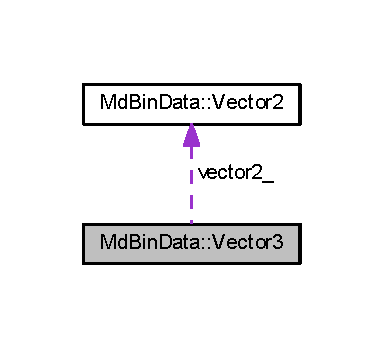
\includegraphics[width=184pt]{class_md_bin_data_1_1_vector3__coll__graph}
\end{center}
\end{figure}
\subsection*{公開メンバ関数}
\begin{DoxyCompactItemize}
\item 
float $\ast$ \mbox{\hyperlink{class_md_bin_data_1_1_vector3_a92662563dc33035c94d457cd96d7972e}{getpX}} ()
\begin{DoxyCompactList}\small\item\em X成分取得関数 \end{DoxyCompactList}\item 
float $\ast$ \mbox{\hyperlink{class_md_bin_data_1_1_vector3_aaf3534a3038219e74875d002255e0c27}{getpY}} ()
\begin{DoxyCompactList}\small\item\em Y成分取得関数 \end{DoxyCompactList}\item 
float $\ast$ \mbox{\hyperlink{class_md_bin_data_1_1_vector3_a3f0b7ef217f5a065fa86aa3da983b6a4}{getpZ}} ()
\begin{DoxyCompactList}\small\item\em Z成分取得関数 \end{DoxyCompactList}\end{DoxyCompactItemize}
\subsection*{非公開メンバ関数}
\begin{DoxyCompactItemize}
\item 
{\footnotesize template$<$class Archive $>$ }\\void \mbox{\hyperlink{class_md_bin_data_1_1_vector3_af1b8febb3546990575e4b6ba7496b619}{serialize}} (Archive \&archive, const unsigned version)
\end{DoxyCompactItemize}
\subsection*{非公開変数類}
\begin{DoxyCompactItemize}
\item 
\mbox{\hyperlink{class_md_bin_data_1_1_vector2}{Vector2}} \mbox{\hyperlink{class_md_bin_data_1_1_vector3_a312b71252e8b585d01c6aaade102b8bc}{vector2\+\_\+}}
\begin{DoxyCompactList}\small\item\em ベクター2 \end{DoxyCompactList}\item 
float \mbox{\hyperlink{class_md_bin_data_1_1_vector3_a5bf432978dbd9411afe66e69fd8aaaef}{z\+\_\+}}
\begin{DoxyCompactList}\small\item\em Z成分 \end{DoxyCompactList}\end{DoxyCompactItemize}
\subsection*{フレンド}
\begin{DoxyCompactItemize}
\item 
class \mbox{\hyperlink{class_md_bin_data_1_1_vector3_ac98d07dd8f7b70e16ccb9a01abf56b9c}{boost\+::serialization\+::access}}
\begin{DoxyCompactList}\small\item\em シリアライズ(I/O)関数 \end{DoxyCompactList}\end{DoxyCompactItemize}


\subsection{詳解}
ベクター3\+Class 

float変数を3つもつ\+Class 

 Md\+Bin\+Data.\+h の 98 行目に定義があります。



\subsection{関数詳解}
\mbox{\Hypertarget{class_md_bin_data_1_1_vector3_a92662563dc33035c94d457cd96d7972e}\label{class_md_bin_data_1_1_vector3_a92662563dc33035c94d457cd96d7972e}} 
\index{Md\+Bin\+Data\+::\+Vector3@{Md\+Bin\+Data\+::\+Vector3}!getpX@{getpX}}
\index{getpX@{getpX}!Md\+Bin\+Data\+::\+Vector3@{Md\+Bin\+Data\+::\+Vector3}}
\subsubsection{\texorpdfstring{getp\+X()}{getpX()}}
{\footnotesize\ttfamily float $\ast$ Md\+Bin\+Data\+::\+Vector3\+::getpX (\begin{DoxyParamCaption}{ }\end{DoxyParamCaption})}



X成分取得関数 


\begin{DoxyParams}{引数}
{\em void} & なし \\
\hline
\end{DoxyParams}

\begin{DoxyRetVals}{戻り値}
{\em float$\ast$} & X成分 \\
\hline
\end{DoxyRetVals}


 Md\+Bin\+Data.\+cpp の 75 行目に定義があります。

\mbox{\Hypertarget{class_md_bin_data_1_1_vector3_aaf3534a3038219e74875d002255e0c27}\label{class_md_bin_data_1_1_vector3_aaf3534a3038219e74875d002255e0c27}} 
\index{Md\+Bin\+Data\+::\+Vector3@{Md\+Bin\+Data\+::\+Vector3}!getpY@{getpY}}
\index{getpY@{getpY}!Md\+Bin\+Data\+::\+Vector3@{Md\+Bin\+Data\+::\+Vector3}}
\subsubsection{\texorpdfstring{getp\+Y()}{getpY()}}
{\footnotesize\ttfamily float $\ast$ Md\+Bin\+Data\+::\+Vector3\+::getpY (\begin{DoxyParamCaption}{ }\end{DoxyParamCaption})}



Y成分取得関数 


\begin{DoxyParams}{引数}
{\em void} & なし \\
\hline
\end{DoxyParams}

\begin{DoxyRetVals}{戻り値}
{\em float$\ast$} & Y成分 \\
\hline
\end{DoxyRetVals}


 Md\+Bin\+Data.\+cpp の 82 行目に定義があります。

\mbox{\Hypertarget{class_md_bin_data_1_1_vector3_a3f0b7ef217f5a065fa86aa3da983b6a4}\label{class_md_bin_data_1_1_vector3_a3f0b7ef217f5a065fa86aa3da983b6a4}} 
\index{Md\+Bin\+Data\+::\+Vector3@{Md\+Bin\+Data\+::\+Vector3}!getpZ@{getpZ}}
\index{getpZ@{getpZ}!Md\+Bin\+Data\+::\+Vector3@{Md\+Bin\+Data\+::\+Vector3}}
\subsubsection{\texorpdfstring{getp\+Z()}{getpZ()}}
{\footnotesize\ttfamily float $\ast$ Md\+Bin\+Data\+::\+Vector3\+::getpZ (\begin{DoxyParamCaption}{ }\end{DoxyParamCaption})}



Z成分取得関数 


\begin{DoxyParams}{引数}
{\em void} & なし \\
\hline
\end{DoxyParams}

\begin{DoxyRetVals}{戻り値}
{\em float$\ast$} & Z成分 \\
\hline
\end{DoxyRetVals}


 Md\+Bin\+Data.\+cpp の 89 行目に定義があります。

\mbox{\Hypertarget{class_md_bin_data_1_1_vector3_af1b8febb3546990575e4b6ba7496b619}\label{class_md_bin_data_1_1_vector3_af1b8febb3546990575e4b6ba7496b619}} 
\index{Md\+Bin\+Data\+::\+Vector3@{Md\+Bin\+Data\+::\+Vector3}!serialize@{serialize}}
\index{serialize@{serialize}!Md\+Bin\+Data\+::\+Vector3@{Md\+Bin\+Data\+::\+Vector3}}
\subsubsection{\texorpdfstring{serialize()}{serialize()}}
{\footnotesize\ttfamily template$<$class Archive $>$ \\
void Md\+Bin\+Data\+::\+Vector3\+::serialize (\begin{DoxyParamCaption}\item[{Archive \&}]{archive,  }\item[{const unsigned}]{version }\end{DoxyParamCaption})\hspace{0.3cm}{\ttfamily [inline]}, {\ttfamily [private]}}



 Md\+Bin\+Data.\+h の 150 行目に定義があります。



\subsection{フレンドと関連関数の詳解}
\mbox{\Hypertarget{class_md_bin_data_1_1_vector3_ac98d07dd8f7b70e16ccb9a01abf56b9c}\label{class_md_bin_data_1_1_vector3_ac98d07dd8f7b70e16ccb9a01abf56b9c}} 
\index{Md\+Bin\+Data\+::\+Vector3@{Md\+Bin\+Data\+::\+Vector3}!boost\+::serialization\+::access@{boost\+::serialization\+::access}}
\index{boost\+::serialization\+::access@{boost\+::serialization\+::access}!Md\+Bin\+Data\+::\+Vector3@{Md\+Bin\+Data\+::\+Vector3}}
\subsubsection{\texorpdfstring{boost\+::serialization\+::access}{boost::serialization::access}}
{\footnotesize\ttfamily friend class boost\+::serialization\+::access\hspace{0.3cm}{\ttfamily [friend]}}



シリアライズ(I/O)関数 


\begin{DoxyParams}{引数}
{\em archive} & アーカイブ用クラス \\
\hline
{\em version} & バージョン \\
\hline
\end{DoxyParams}

\begin{DoxyRetVals}{戻り値}
{\em void} & なし \\
\hline
\end{DoxyRetVals}


 Md\+Bin\+Data.\+h の 148 行目に定義があります。



\subsection{メンバ詳解}
\mbox{\Hypertarget{class_md_bin_data_1_1_vector3_a312b71252e8b585d01c6aaade102b8bc}\label{class_md_bin_data_1_1_vector3_a312b71252e8b585d01c6aaade102b8bc}} 
\index{Md\+Bin\+Data\+::\+Vector3@{Md\+Bin\+Data\+::\+Vector3}!vector2\+\_\+@{vector2\+\_\+}}
\index{vector2\+\_\+@{vector2\+\_\+}!Md\+Bin\+Data\+::\+Vector3@{Md\+Bin\+Data\+::\+Vector3}}
\subsubsection{\texorpdfstring{vector2\+\_\+}{vector2\_}}
{\footnotesize\ttfamily \mbox{\hyperlink{class_md_bin_data_1_1_vector2}{Vector2}} Md\+Bin\+Data\+::\+Vector3\+::vector2\+\_\+\hspace{0.3cm}{\ttfamily [private]}}



ベクター2 



 Md\+Bin\+Data.\+h の 104 行目に定義があります。

\mbox{\Hypertarget{class_md_bin_data_1_1_vector3_a5bf432978dbd9411afe66e69fd8aaaef}\label{class_md_bin_data_1_1_vector3_a5bf432978dbd9411afe66e69fd8aaaef}} 
\index{Md\+Bin\+Data\+::\+Vector3@{Md\+Bin\+Data\+::\+Vector3}!z\+\_\+@{z\+\_\+}}
\index{z\+\_\+@{z\+\_\+}!Md\+Bin\+Data\+::\+Vector3@{Md\+Bin\+Data\+::\+Vector3}}
\subsubsection{\texorpdfstring{z\+\_\+}{z\_}}
{\footnotesize\ttfamily float Md\+Bin\+Data\+::\+Vector3\+::z\+\_\+\hspace{0.3cm}{\ttfamily [private]}}



Z成分 



 Md\+Bin\+Data.\+h の 105 行目に定義があります。



このクラス詳解は次のファイルから抽出されました\+:\begin{DoxyCompactItemize}
\item 
C\+:/\+H\+A\+L/\+P\+G関係/03\+\_\+作成プログラム/03\+\_\+\+H\+A\+L授業/就職作品/\+Fbx\+Converter/source/\+Md\+Bin\+Data/\mbox{\hyperlink{_md_bin_data_8h}{Md\+Bin\+Data.\+h}}\item 
C\+:/\+H\+A\+L/\+P\+G関係/03\+\_\+作成プログラム/03\+\_\+\+H\+A\+L授業/就職作品/\+Fbx\+Converter/source/\+Md\+Bin\+Data/\mbox{\hyperlink{_md_bin_data_8cpp}{Md\+Bin\+Data.\+cpp}}\end{DoxyCompactItemize}

\chapter{ファイル詳解}
\hypertarget{main__page_8txt}{}\section{main\+\_\+page/main\+\_\+page.txt ファイル}
\label{main__page_8txt}\index{main\+\_\+page/main\+\_\+page.\+txt@{main\+\_\+page/main\+\_\+page.\+txt}}

\hypertarget{_export_file_8cpp}{}\section{C\+:/\+H\+A\+L/\+P\+G関係/03\+\_\+作成プログラム/03\+\_\+\+H\+A\+L授業/就職作品/\+Fbx\+Converter/source/\+Export\+File/\+Export\+File.cpp ファイル}
\label{_export_file_8cpp}\index{C\+:/\+H\+A\+L/\+P\+G関係/03\+\_\+作成プログラム/03\+\_\+\+H\+A\+L授業/就職作品/\+Fbx\+Converter/source/\+Export\+File/\+Export\+File.\+cpp@{C\+:/\+H\+A\+L/\+P\+G関係/03\+\_\+作成プログラム/03\+\_\+\+H\+A\+L授業/就職作品/\+Fbx\+Converter/source/\+Export\+File/\+Export\+File.\+cpp}}


ファイル出力\+Class  


{\ttfamily \#include $<$iostream$>$}\newline
{\ttfamily \#include $<$fstream$>$}\newline
{\ttfamily \#include $<$windows.\+h$>$}\newline
{\ttfamily \#include $<$imagehlp.\+h$>$}\newline
{\ttfamily \#include $<$stdio.\+h$>$}\newline
{\ttfamily \#include $<$shlwapi.\+h$>$}\newline
{\ttfamily \#include \char`\"{}Export\+File.\+h\char`\"{}}\newline


\subsection{詳解}
ファイル出力\+Class 

\begin{DoxyAuthor}{著者}
Kai Araki 
\end{DoxyAuthor}
\begin{DoxyDate}{日付}
2019/01/22 
\end{DoxyDate}

\hypertarget{_export_file_8h}{}\section{C\+:/\+H\+A\+L/\+P\+G関係/03\+\_\+作成プログラム/03\+\_\+\+H\+A\+L授業/就職作品/\+Fbx\+Converter/source/\+Export\+File/\+Export\+File.h ファイル}
\label{_export_file_8h}\index{C\+:/\+H\+A\+L/\+P\+G関係/03\+\_\+作成プログラム/03\+\_\+\+H\+A\+L授業/就職作品/\+Fbx\+Converter/source/\+Export\+File/\+Export\+File.\+h@{C\+:/\+H\+A\+L/\+P\+G関係/03\+\_\+作成プログラム/03\+\_\+\+H\+A\+L授業/就職作品/\+Fbx\+Converter/source/\+Export\+File/\+Export\+File.\+h}}


ファイル出力\+Class  


{\ttfamily \#include $<$fbxsdk.\+h$>$}\newline
{\ttfamily \#include $<$string$>$}\newline
{\ttfamily \#include \char`\"{}../\+Md\+Bin\+Data/\+Md\+Bin\+Data.\+h\char`\"{}}\newline
\subsection*{クラス}
\begin{DoxyCompactItemize}
\item 
class \mbox{\hyperlink{class_export_file}{Export\+File}}
\begin{DoxyCompactList}\small\item\em ファイル出力\+Class \end{DoxyCompactList}\end{DoxyCompactItemize}


\subsection{詳解}
ファイル出力\+Class 

License \+: M\+IT \begin{DoxyAuthor}{著者}
Kai Araki 
\end{DoxyAuthor}
\begin{DoxyDate}{日付}
2019/01/22 
\end{DoxyDate}

\hypertarget{_fbx_converter_8cpp}{}\section{C\+:/\+H\+A\+L/\+P\+G関係/03\+\_\+作成プログラム/03\+\_\+\+H\+A\+L授業/就職作品/\+Fbx\+Converter/source/\+Fbx\+Converter/\+Fbx\+Converter.cpp ファイル}
\label{_fbx_converter_8cpp}\index{C\+:/\+H\+A\+L/\+P\+G関係/03\+\_\+作成プログラム/03\+\_\+\+H\+A\+L授業/就職作品/\+Fbx\+Converter/source/\+Fbx\+Converter/\+Fbx\+Converter.\+cpp@{C\+:/\+H\+A\+L/\+P\+G関係/03\+\_\+作成プログラム/03\+\_\+\+H\+A\+L授業/就職作品/\+Fbx\+Converter/source/\+Fbx\+Converter/\+Fbx\+Converter.\+cpp}}


F\+B\+X変換器\+Class  


{\ttfamily \#include $<$iostream$>$}\newline
{\ttfamily \#include \char`\"{}Fbx\+Converter.\+h\char`\"{}}\newline


\subsection{詳解}
F\+B\+X変換器\+Class 

License \+: M\+IT \begin{DoxyAuthor}{著者}
Kai Araki 
\end{DoxyAuthor}
\begin{DoxyDate}{日付}
2018/12/29 
\end{DoxyDate}

\hypertarget{_fbx_converter_8h}{}\section{C\+:/\+H\+A\+L/\+P\+G関係/03\+\_\+作成プログラム/03\+\_\+\+H\+A\+L授業/就職作品/\+Fbx\+Converter/source/\+Fbx\+Converter/\+Fbx\+Converter.h ファイル}
\label{_fbx_converter_8h}\index{C\+:/\+H\+A\+L/\+P\+G関係/03\+\_\+作成プログラム/03\+\_\+\+H\+A\+L授業/就職作品/\+Fbx\+Converter/source/\+Fbx\+Converter/\+Fbx\+Converter.\+h@{C\+:/\+H\+A\+L/\+P\+G関係/03\+\_\+作成プログラム/03\+\_\+\+H\+A\+L授業/就職作品/\+Fbx\+Converter/source/\+Fbx\+Converter/\+Fbx\+Converter.\+h}}


F\+B\+X変換器\+Class  


{\ttfamily \#include $<$fbxsdk.\+h$>$}\newline
{\ttfamily \#include $<$string$>$}\newline
{\ttfamily \#include \char`\"{}../\+Md\+Bin\+Data/\+Md\+Bin\+Data.\+h\char`\"{}}\newline
{\ttfamily \#include \char`\"{}../\+Export\+File/\+Export\+File.\+h\char`\"{}}\newline
\subsection*{クラス}
\begin{DoxyCompactItemize}
\item 
class \mbox{\hyperlink{class_fbx_converter}{Fbx\+Converter}}
\begin{DoxyCompactList}\small\item\em F\+B\+X変換器\+Class \end{DoxyCompactList}\end{DoxyCompactItemize}


\subsection{詳解}
F\+B\+X変換器\+Class 

License \+: M\+IT \begin{DoxyAuthor}{著者}
Kai Araki 
\end{DoxyAuthor}
\begin{DoxyDate}{日付}
2018/12/29 
\end{DoxyDate}

\hypertarget{main_8cpp}{}\section{C\+:/\+H\+A\+L/\+P\+G関係/03\+\_\+作成プログラム/03\+\_\+\+H\+A\+L授業/就職作品/\+Fbx\+Converter/source/main.cpp ファイル}
\label{main_8cpp}\index{C\+:/\+H\+A\+L/\+P\+G関係/03\+\_\+作成プログラム/03\+\_\+\+H\+A\+L授業/就職作品/\+Fbx\+Converter/source/main.\+cpp@{C\+:/\+H\+A\+L/\+P\+G関係/03\+\_\+作成プログラム/03\+\_\+\+H\+A\+L授業/就職作品/\+Fbx\+Converter/source/main.\+cpp}}


メイン  


{\ttfamily \#include $<$crtdbg.\+h$>$}\newline
{\ttfamily \#include $<$stdio.\+h$>$}\newline
{\ttfamily \#include $<$stdlib.\+h$>$}\newline
{\ttfamily \#include $<$iostream$>$}\newline
{\ttfamily \#include \char`\"{}Fbx\+Converter/\+Fbx\+Converter.\+h\char`\"{}}\newline
\subsection*{関数}
\begin{DoxyCompactItemize}
\item 
int \mbox{\hyperlink{main_8cpp_a840291bc02cba5474a4cb46a9b9566fe}{main}} (void)
\end{DoxyCompactItemize}


\subsection{詳解}
メイン 

\begin{DoxyAuthor}{著者}
Kai Araki 
\end{DoxyAuthor}
\begin{DoxyDate}{日付}
2018/12/12 
\end{DoxyDate}


\subsection{関数詳解}
\mbox{\Hypertarget{main_8cpp_a840291bc02cba5474a4cb46a9b9566fe}\label{main_8cpp_a840291bc02cba5474a4cb46a9b9566fe}} 
\index{main.\+cpp@{main.\+cpp}!main@{main}}
\index{main@{main}!main.\+cpp@{main.\+cpp}}
\subsubsection{\texorpdfstring{main()}{main()}}
{\footnotesize\ttfamily int main (\begin{DoxyParamCaption}\item[{void}]{ }\end{DoxyParamCaption})}



 main.\+cpp の 25 行目に定義があります。


\hypertarget{_md_bin_data_8cpp}{}\section{C\+:/\+H\+A\+L/\+P\+G関係/03\+\_\+作成プログラム/03\+\_\+\+H\+A\+L授業/就職作品/\+Fbx\+Converter/source/\+Md\+Bin\+Data/\+Md\+Bin\+Data.cpp ファイル}
\label{_md_bin_data_8cpp}\index{C\+:/\+H\+A\+L/\+P\+G関係/03\+\_\+作成プログラム/03\+\_\+\+H\+A\+L授業/就職作品/\+Fbx\+Converter/source/\+Md\+Bin\+Data/\+Md\+Bin\+Data.\+cpp@{C\+:/\+H\+A\+L/\+P\+G関係/03\+\_\+作成プログラム/03\+\_\+\+H\+A\+L授業/就職作品/\+Fbx\+Converter/source/\+Md\+Bin\+Data/\+Md\+Bin\+Data.\+cpp}}


バイナリーモデルデータ\+Class  


{\ttfamily \#include $<$fstream$>$}\newline
{\ttfamily \#include $<$boost/archive/binary\+\_\+oarchive.\+hpp$>$}\newline
{\ttfamily \#include $<$boost/archive/binary\+\_\+iarchive.\+hpp$>$}\newline
{\ttfamily \#include \char`\"{}Md\+Bin\+Data.\+h\char`\"{}}\newline


\subsection{詳解}
バイナリーモデルデータ\+Class 

\begin{DoxyAuthor}{著者}
Kai Araki 
\end{DoxyAuthor}
\begin{DoxyDate}{日付}
2018/12/29 
\end{DoxyDate}

\hypertarget{_md_bin_data_8h}{}\section{C\+:/\+H\+A\+L/\+P\+G関係/03\+\_\+作成プログラム/03\+\_\+\+H\+A\+L授業/就職作品/\+Fbx\+Converter/source/\+Md\+Bin\+Data/\+Md\+Bin\+Data.h ファイル}
\label{_md_bin_data_8h}\index{C\+:/\+H\+A\+L/\+P\+G関係/03\+\_\+作成プログラム/03\+\_\+\+H\+A\+L授業/就職作品/\+Fbx\+Converter/source/\+Md\+Bin\+Data/\+Md\+Bin\+Data.\+h@{C\+:/\+H\+A\+L/\+P\+G関係/03\+\_\+作成プログラム/03\+\_\+\+H\+A\+L授業/就職作品/\+Fbx\+Converter/source/\+Md\+Bin\+Data/\+Md\+Bin\+Data.\+h}}


バイナリーモデルデータ\+Class  


{\ttfamily \#include $<$stdio.\+h$>$}\newline
{\ttfamily \#include $<$vector$>$}\newline
{\ttfamily \#include $<$string$>$}\newline
{\ttfamily \#include $<$boost/serialization/serialization.\+hpp$>$}\newline
{\ttfamily \#include $<$boost/serialization/string.\+hpp$>$}\newline
{\ttfamily \#include $<$boost/serialization/vector.\+hpp$>$}\newline
\subsection*{クラス}
\begin{DoxyCompactItemize}
\item 
class \mbox{\hyperlink{class_md_bin_data}{Md\+Bin\+Data}}
\begin{DoxyCompactList}\small\item\em バイナリーモデルデータ\+Class \end{DoxyCompactList}\item 
class \mbox{\hyperlink{class_md_bin_data_1_1_vector2}{Md\+Bin\+Data\+::\+Vector2}}
\begin{DoxyCompactList}\small\item\em ベクター2\+Class \end{DoxyCompactList}\item 
class \mbox{\hyperlink{class_md_bin_data_1_1_vector3}{Md\+Bin\+Data\+::\+Vector3}}
\begin{DoxyCompactList}\small\item\em ベクター3\+Class \end{DoxyCompactList}\item 
class \mbox{\hyperlink{class_md_bin_data_1_1_color}{Md\+Bin\+Data\+::\+Color}}
\begin{DoxyCompactList}\small\item\em 色\+Class \end{DoxyCompactList}\item 
class \mbox{\hyperlink{class_md_bin_data_1_1_matrix}{Md\+Bin\+Data\+::\+Matrix}}
\begin{DoxyCompactList}\small\item\em 行列\+Class \end{DoxyCompactList}\item 
class \mbox{\hyperlink{class_md_bin_data_1_1_material}{Md\+Bin\+Data\+::\+Material}}
\begin{DoxyCompactList}\small\item\em マテリアル\+Class \end{DoxyCompactList}\item 
class \mbox{\hyperlink{class_md_bin_data_1_1_material_1_1_texture}{Md\+Bin\+Data\+::\+Material\+::\+Texture}}
\begin{DoxyCompactList}\small\item\em テクスチャ\+Class \end{DoxyCompactList}\item 
class \mbox{\hyperlink{class_md_bin_data_1_1_mesh}{Md\+Bin\+Data\+::\+Mesh}}
\begin{DoxyCompactList}\small\item\em メッシュ\+Class \end{DoxyCompactList}\item 
class \mbox{\hyperlink{class_md_bin_data_1_1_mesh_1_1_u_v_set}{Md\+Bin\+Data\+::\+Mesh\+::\+U\+V\+Set}}
\begin{DoxyCompactList}\small\item\em U\+Vセット\+Class \end{DoxyCompactList}\item 
class \mbox{\hyperlink{class_md_bin_data_1_1_mesh_1_1_bone}{Md\+Bin\+Data\+::\+Mesh\+::\+Bone}}
\begin{DoxyCompactList}\small\item\em ボーン\+Class \end{DoxyCompactList}\item 
class \mbox{\hyperlink{class_md_bin_data_1_1_mesh_1_1_bone_weight}{Md\+Bin\+Data\+::\+Mesh\+::\+Bone\+Weight}}
\begin{DoxyCompactList}\small\item\em ボーン重み\+Class \end{DoxyCompactList}\end{DoxyCompactItemize}


\subsection{詳解}
バイナリーモデルデータ\+Class 

License \+: M\+IT \begin{DoxyAuthor}{著者}
Kai Araki 
\end{DoxyAuthor}
\begin{DoxyDate}{日付}
2018/12/29 
\end{DoxyDate}

%--- End generated contents ---

% Index
\backmatter
\newpage
\phantomsection
\clearemptydoublepage
\addcontentsline{toc}{chapter}{索引}
\printindex

\end{document}
